\documentclass[11pt]{article}
\usepackage[margin=2cm]{geometry}
\usepackage{amsmath,amssymb}
\usepackage{graphicx}
\usepackage{booktabs}
\usepackage{array}
\usepackage{xcolor}
\usepackage[breakable]{tcolorbox}
\usepackage{enumitem}
\usepackage[hidelinks]{hyperref}
\allowdisplaybreaks
\setlength{\parindent}{0pt}
\setlength{\parskip}{4pt}
\definecolor{stepc}{HTML}{1F4E9E}
\definecolor{ansc}{HTML}{0B6E4F}
\newcommand{\solstep}[2]{\par\medskip{\color{stepc}\textbf{Step #1 --- #2}}\par\nopagebreak}
\newtcolorbox{probbox}[1]{colback=white,colframe=black!55,fonttitle=\bfseries,title={#1}}
\newtcolorbox{ansbox}{breakable,colback=ansc!6,colframe=ansc,fonttitle=\bfseries,title={Answer}}
\newtcolorbox{cardbox}[1]{breakable,colback=stepc!4,colframe=stepc,fonttitle=\bfseries,title={#1}}
\graphicspath{{../../../output/lecture1/1C_dependent_sources/}}
\title{Set 1C: Stages Coupled by Dependent Sources}
\author{ECEN 325 --- Lecture 1 (Linear Network Analysis) practice set}
\date{}
\begin{document}
\maketitle

\textbf{What this set trains.} Circuits split into stages by dependent sources (diamond symbols). A VCVS
($kV_x$) forces its output voltage; a VCCS ($gV_x$) pushes a current into the impedance on its node. Because a
dependent source does not load the node it watches, $H(s)$ is simply the product of the stage gains, and each
stage is solved with voltage dividers. Problems 1--6 are easy, 7--12 medium, 13--18 hard. Try each problem
before looking at its solution.


\begin{cardbox}{The Lecture-1 pipeline (use it for every problem in this set)}
\textbf{Tools --- this is all the theory you need:}
\begin{enumerate}[label=\textbf{T\arabic*},leftmargin=2.2em,itemsep=1pt]
\item \emph{Impedances:} $Z_R=R$, $Z_C=\frac{1}{sC}$, $Z_L=sL$. Series: add. Parallel:
      $Z_a\parallel Z_b=\frac{Z_aZ_b}{Z_a+Z_b}$.
\item \emph{Voltage divider:} if $Z_{top}$ connects $V_{in}$ to a node and $Z_{bot}$ is everything from that
      node to ground, then $V_{node}=V_{in}\,\frac{Z_{bot}}{Z_{top}+Z_{bot}}$.
\item \emph{Divider between two voltages (DC):} a node tied to $V_a$ through $R_a$ and to $V_b$ through $R_b$ sits at
      $V=V_b+(V_a-V_b)\frac{R_b}{R_a+R_b}$, and looks like a source $V$ with resistance $R_a\parallel R_b$
      (its Thevenin pair).
\item \emph{Dependent sources:} a VCVS forces $V=kV_x$; a VCCS drives the current $gV_x$ through the impedance $Z$
      hanging on its node, so $V=\pm gV_x Z$ (sign from the arrow).
\item \emph{Sinusoids:} $A\sin(\omega t+\theta)\ \to\ |H(j\omega)|\,A\sin\big(\omega t+\theta+\angle H(j\omega)\big)$.
\item \emph{Bode rules:} a pole at $p$ bends the magnitude by $-20$\,dB/dec above $p$, a zero by $+20$\,dB/dec;
      $\frac{1}{1+s/p}$ is $0$\,dB below $p$; $\frac{s}{s+p}$ is $0$\,dB above $p$.
\end{enumerate}
\textbf{Steps:}
\begin{enumerate}[leftmargin=2.2em,itemsep=1pt]
\item \emph{Sources.} DC and AC both present $\Rightarrow$ superposition $V_o=V_{o,dc}+v_{o,ac}$.
\item \emph{DC circuit:} $V_i\to0$, $C\to$ open, $L\to$ short; reduce toward $V_o$ with T3.
\item \emph{AC circuit:} DC supplies $\to 0$ (rails become ground); merge parallel resistors.
\item \emph{Divider chain:} name the nodes from $V_i$ to $V_o$; $H=\prod$ (node-to-node ratios), each by T2 or T4,
      using the impedance seen looking right from each node.
\item \emph{Standard form:} simplify, find the roots, write $H=K\cdot\prod(\text{factors})$.
\item \emph{Bode:} start from the low-frequency slope, bend by $\pm20$\,dB/dec at each corner.
\item \emph{Output:} evaluate each factor at $s=j\omega_{in}$, multiply magnitudes, add angles, apply T5 and add $V_{o,dc}$.
\end{enumerate}
\end{cardbox}

\section*{Problems}
\subsection*{Easy problems}
\begin{probbox}{Problem 1C.1 \hfill Easy}
For the circuit below: (a) find the AC transfer function $H(s)=\dfrac{V_o(s)}{V_i(s)}$ and sketch its magnitude Bode plot; (b) find the steady-state output $V_o(t)$ for $V_i(t) = 0.1\sin\left(2\pi\cdot 1000\,t\right)$.
\begin{center}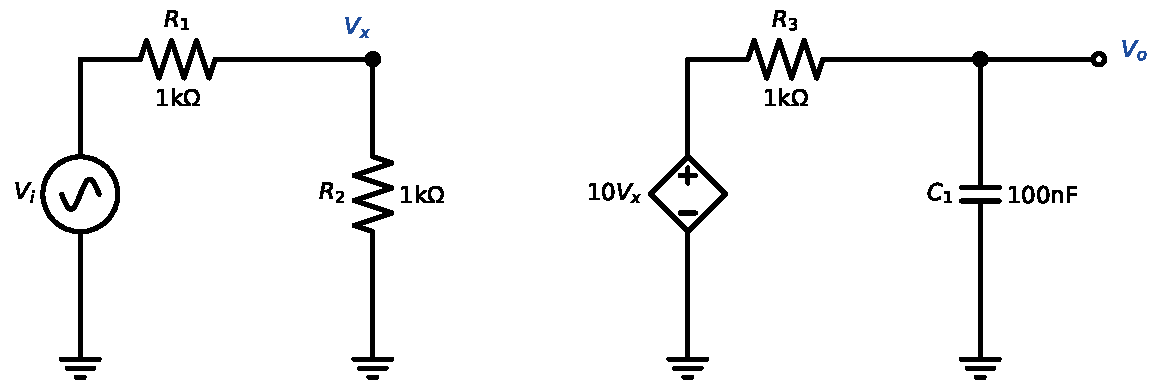
\includegraphics[width=\linewidth,height=5.5cm,keepaspectratio]{p01_circuit}\end{center}
\end{probbox}

\begin{probbox}{Problem 1C.2 \hfill Easy}
For the circuit below: (a) find the AC transfer function $H(s)=\dfrac{V_o(s)}{V_i(s)}$ and sketch its magnitude Bode plot; (b) find the steady-state output $V_o(t)$ for $V_i(t) = 0.2\sin\left(2\pi\cdot 100\,t\right)$.
\begin{center}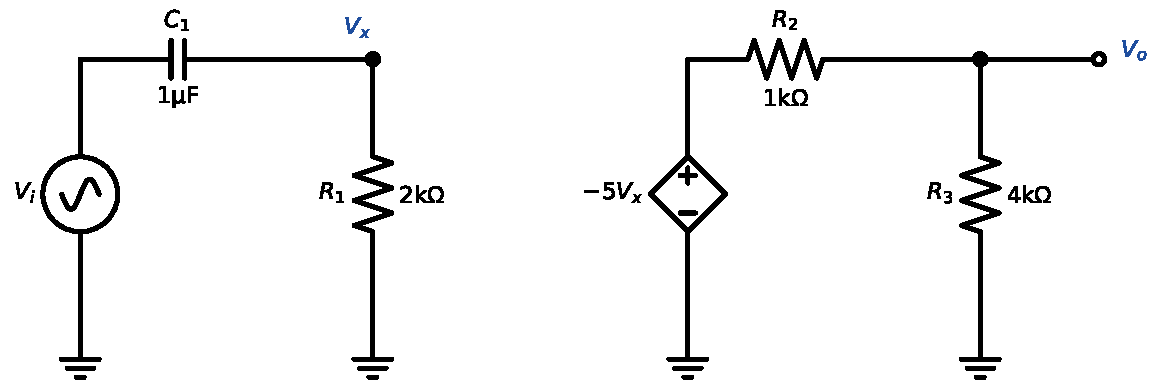
\includegraphics[width=\linewidth,height=5.5cm,keepaspectratio]{p02_circuit}\end{center}
\end{probbox}

\begin{probbox}{Problem 1C.3 \hfill Easy}
For the circuit below: (a) find the AC transfer function $H(s)=\dfrac{V_o(s)}{V_i(s)}$ and sketch its magnitude Bode plot; (b) find the steady-state output $V_o(t)$ for $V_i(t) = 0.05\sin\left(2\pi\cdot 500\,t\right)$.
\begin{center}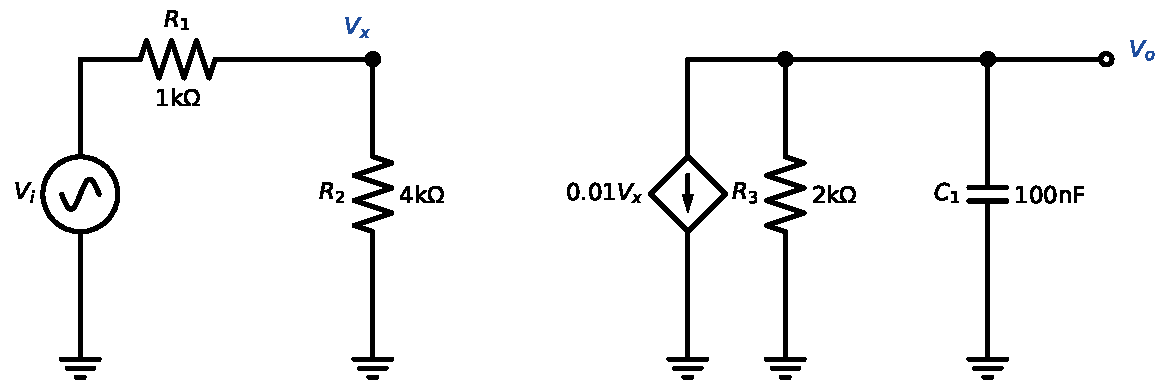
\includegraphics[width=\linewidth,height=5.5cm,keepaspectratio]{p03_circuit}\end{center}
\end{probbox}

\begin{probbox}{Problem 1C.4 \hfill Easy}
For the circuit below: (a) find the AC transfer function $H(s)=\dfrac{V_o(s)}{V_i(s)}$ and sketch its magnitude Bode plot; (b) find the steady-state output $V_o(t)$ for $V_i(t) = 0.1\sin\left(2\pi\cdot 200\,t\right)$.
\begin{center}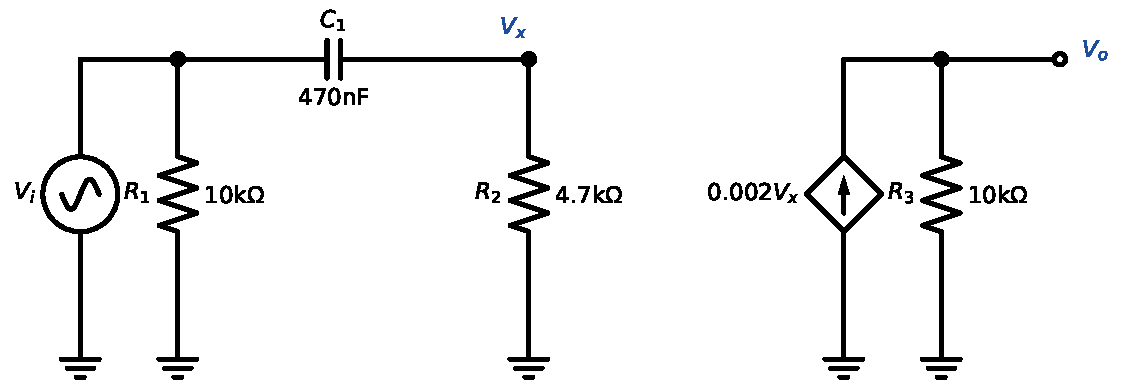
\includegraphics[width=\linewidth,height=5.5cm,keepaspectratio]{p04_circuit}\end{center}
\end{probbox}

\begin{probbox}{Problem 1C.5 \hfill Easy}
For the circuit below: (a) find the AC transfer function $H(s)=\dfrac{V_o(s)}{V_i(s)}$ and sketch its magnitude Bode plot; (b) find the steady-state output $V_o(t)$ for $V_i(t) = 0.05\sin\left(2\pi\cdot 300\,t\right)$.
\begin{center}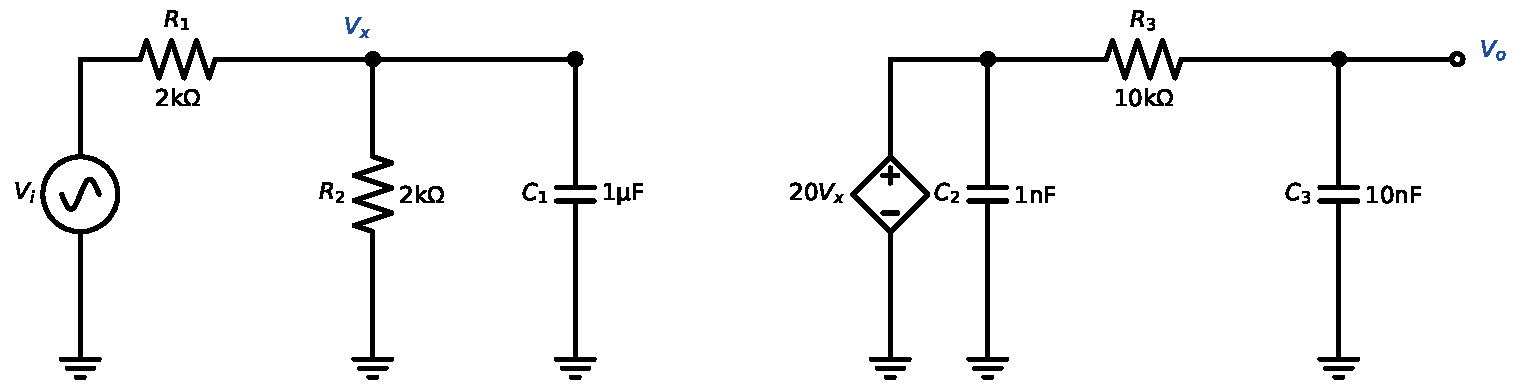
\includegraphics[width=\linewidth,height=5.5cm,keepaspectratio]{p05_circuit}\end{center}
\end{probbox}

\begin{probbox}{Problem 1C.6 \hfill Easy}
For the circuit below: (a) find the AC transfer function $H(s)=\dfrac{V_o(s)}{V_i(s)}$ and sketch its magnitude Bode plot; (b) find the steady-state output $V_o(t)$ for $V_i(t) = 0.2\sin\left(2\pi\cdot 50\,t\right)$.
\begin{center}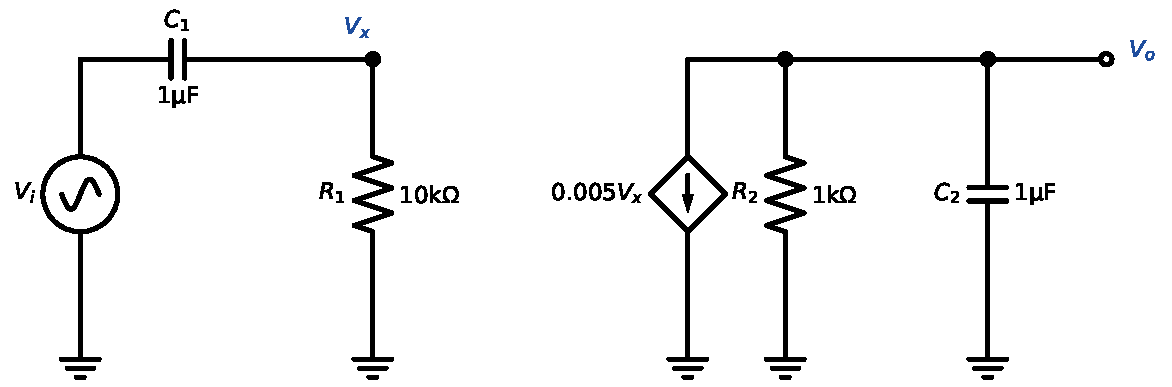
\includegraphics[width=\linewidth,height=5.5cm,keepaspectratio]{p06_circuit}\end{center}
\end{probbox}

\subsection*{Medium problems}
\begin{probbox}{Problem 1C.7 \hfill Medium}
For the circuit below: (a) find the AC transfer function $H(s)=\dfrac{V_o(s)}{V_i(s)}$ and sketch its magnitude Bode plot; (b) find the steady-state output $V_o(t)$ for $V_i(t) = 0.1\sin\left(2\pi\cdot 1000\,t\right)$.
\begin{center}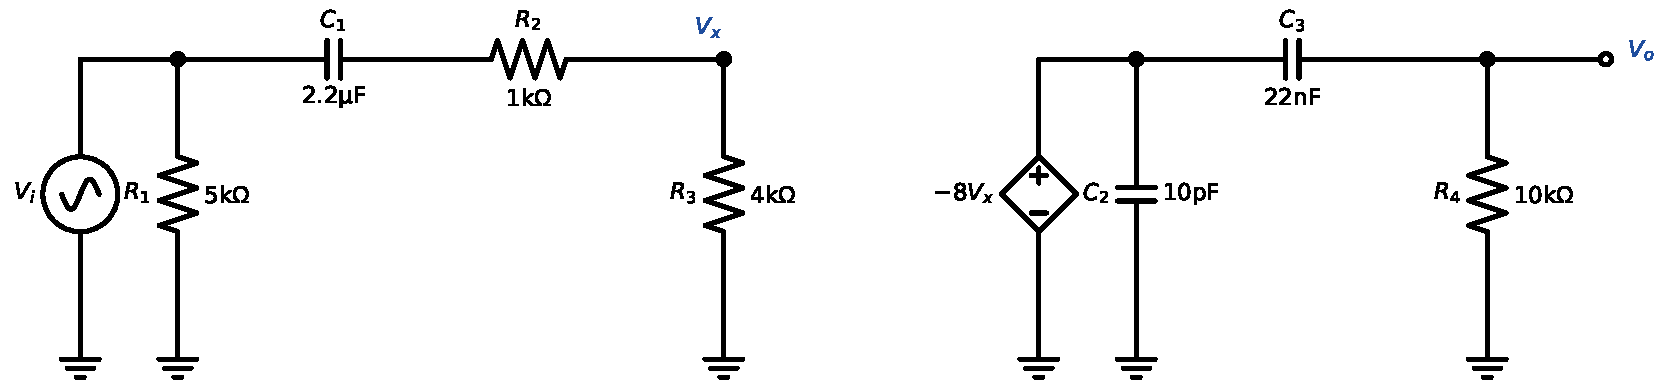
\includegraphics[width=\linewidth,height=5.5cm,keepaspectratio]{p07_circuit}\end{center}
\end{probbox}

\begin{probbox}{Problem 1C.8 \hfill Medium}
For the circuit below: (a) find the AC transfer function $H(s)=\dfrac{V_o(s)}{V_i(s)}$ and sketch its magnitude Bode plot; (b) find the steady-state output $V_o(t)$ for $V_i(t) = 0.05\sin\left(2\pi\cdot 2000\,t\right)$.
\begin{center}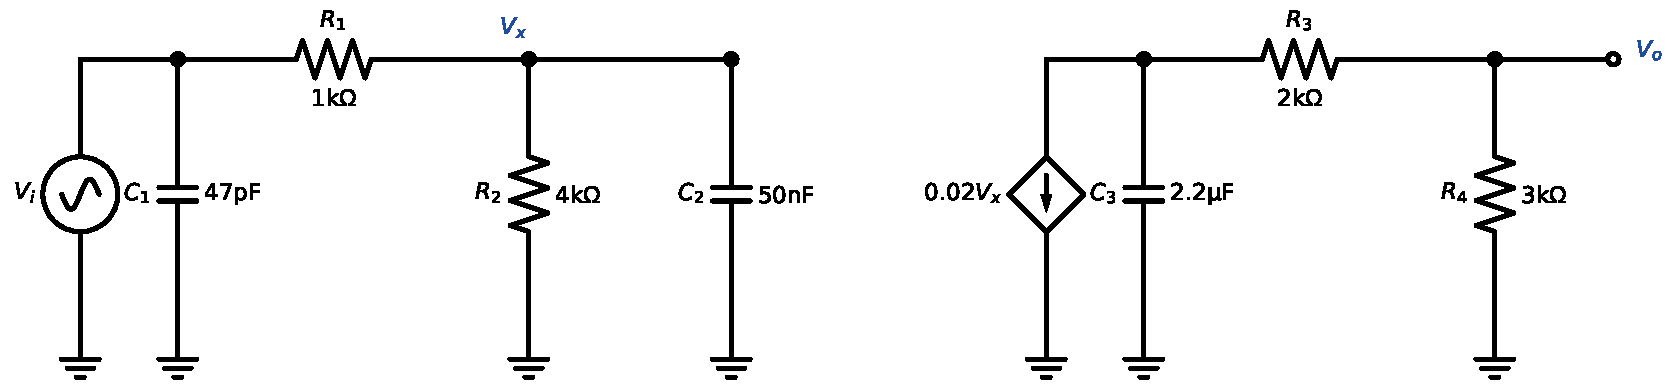
\includegraphics[width=\linewidth,height=5.5cm,keepaspectratio]{p08_circuit}\end{center}
\end{probbox}

\begin{probbox}{Problem 1C.9 \hfill Medium}
For the circuit below: (a) find the AC transfer function $H(s)=\dfrac{V_o(s)}{V_i(s)}$ and sketch its magnitude Bode plot; (b) find the steady-state output $V_o(t)$ for $V_i(t) = 0.2\sin\left(2\pi\cdot 5000\,t\right)$.
\begin{center}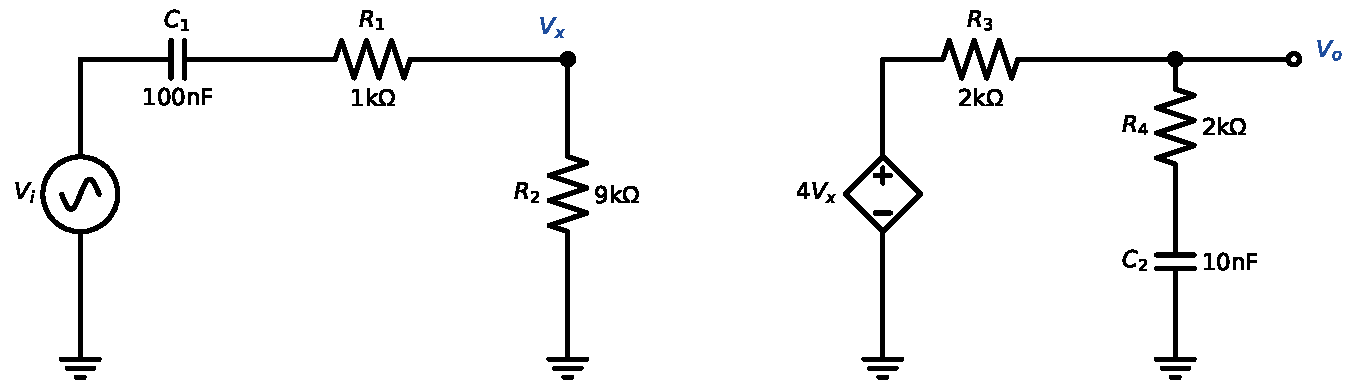
\includegraphics[width=\linewidth,height=5.5cm,keepaspectratio]{p09_circuit}\end{center}
\end{probbox}

\begin{probbox}{Problem 1C.10 \hfill Medium}
For the circuit below: (a) find the AC transfer function $H(s)=\dfrac{V_o(s)}{V_i(s)}$ and sketch its magnitude Bode plot; (b) find the steady-state output $V_o(t)$ for $V_i(t) = 0.5\sin\left(2\pi\cdot 100\,t\right)$.
\begin{center}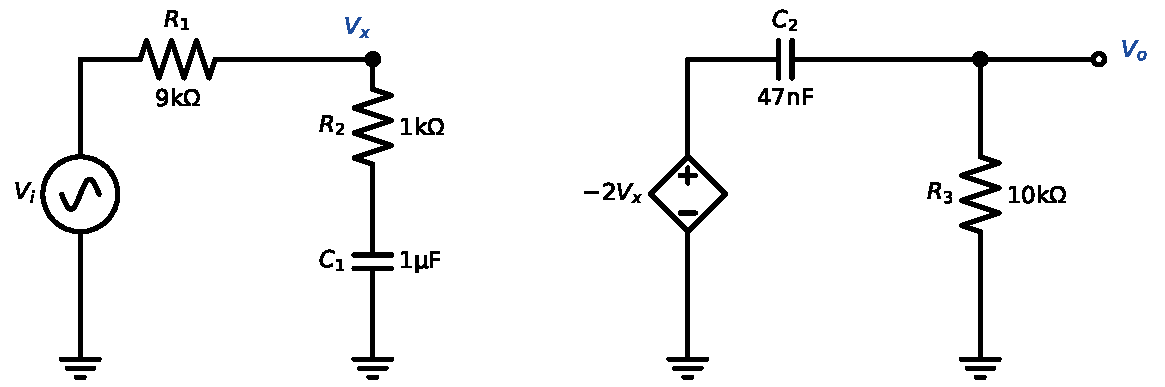
\includegraphics[width=\linewidth,height=5.5cm,keepaspectratio]{p10_circuit}\end{center}
\end{probbox}

\begin{probbox}{Problem 1C.11 \hfill Medium}
For the circuit below: (a) find the AC transfer function $H(s)=\dfrac{V_o(s)}{V_i(s)}$ and sketch its magnitude Bode plot; (b) find the steady-state output $V_o(t)$ for $V_i(t) = 0.2\sin\left(2\pi\cdot 20000\,t\right)$.
\begin{center}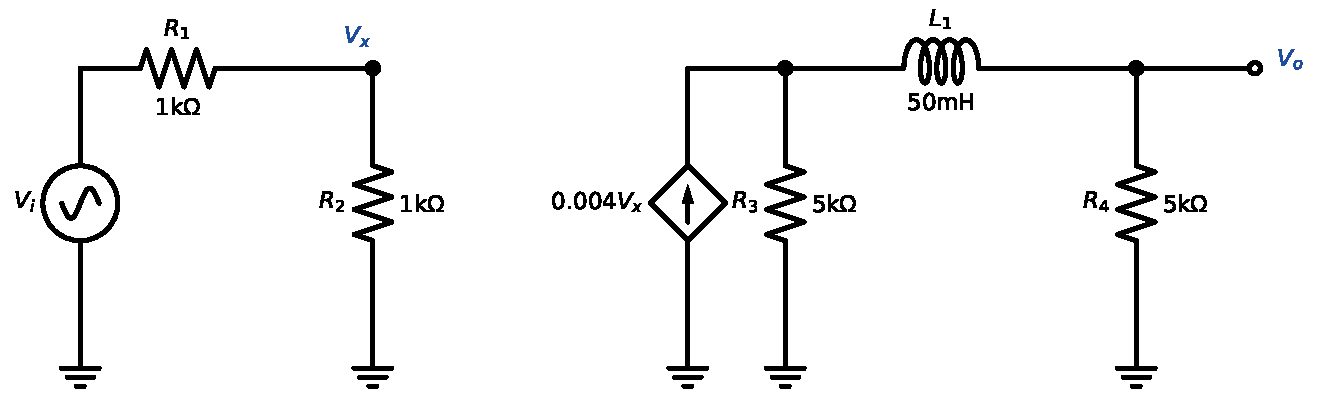
\includegraphics[width=\linewidth,height=5.5cm,keepaspectratio]{p11_circuit}\end{center}
\end{probbox}

\begin{probbox}{Problem 1C.12 \hfill Medium}
For the circuit below: (a) find the AC transfer function $H(s)=\dfrac{V_o(s)}{V_i(s)}$ and sketch its magnitude Bode plot; (b) find the steady-state output $V_o(t)$ for $V_i(t) = 0.1\sin\left(2\pi\cdot 1000\,t\right)$.
\begin{center}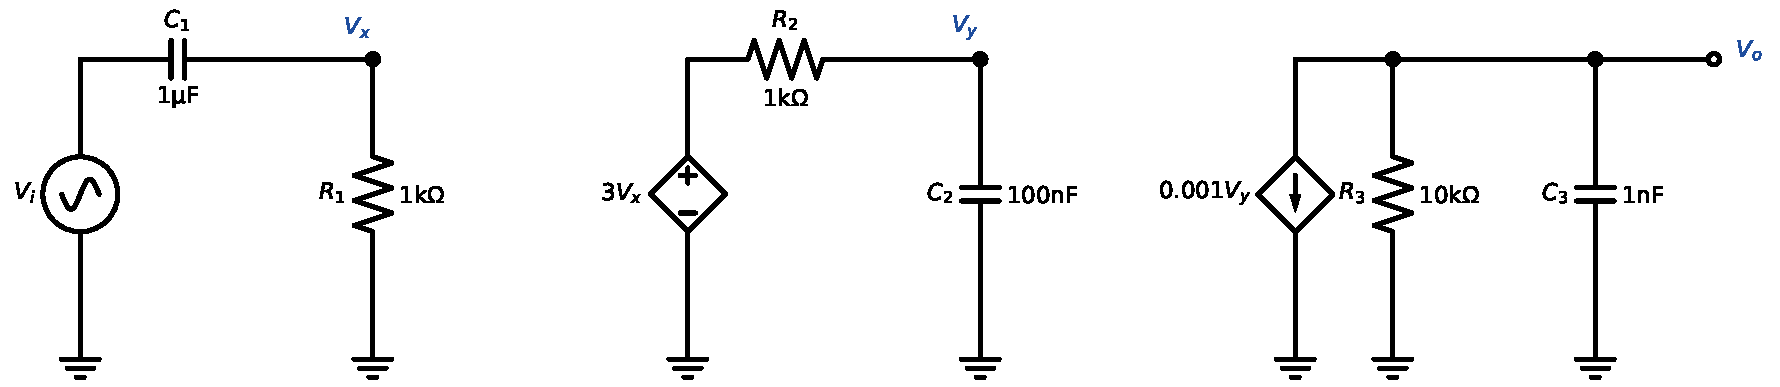
\includegraphics[width=\linewidth,height=5.5cm,keepaspectratio]{p12_circuit}\end{center}
\end{probbox}

\subsection*{Hard problems}
\begin{probbox}{Problem 1C.13 \hfill Hard}
For the circuit below: (a) find the AC transfer function $H(s)=\dfrac{V_o(s)}{V_i(s)}$ and sketch its magnitude Bode plot; (b) find the steady-state output $V_o(t)$ for $V_i(t) = 0.05\sin\left(2\pi\cdot 2000\,t\right)$.
\begin{center}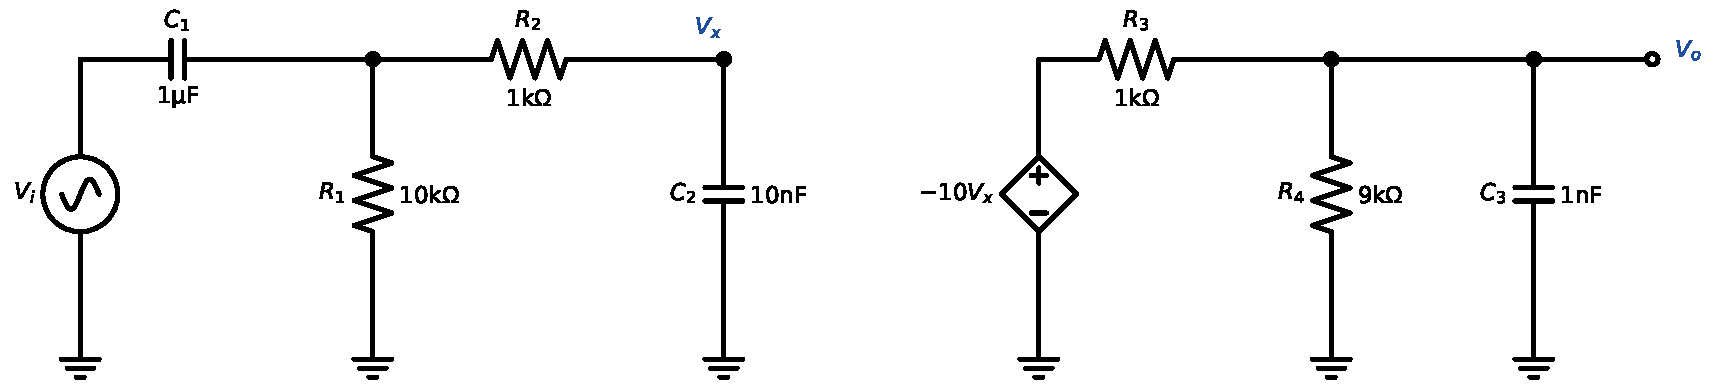
\includegraphics[width=\linewidth,height=5.5cm,keepaspectratio]{p13_circuit}\end{center}
\end{probbox}

\begin{probbox}{Problem 1C.14 \hfill Hard}
For the circuit below: (a) find the AC transfer function $H(s)=\dfrac{V_o(s)}{V_i(s)}$ and sketch its magnitude Bode plot; (b) find the steady-state output $V_o(t)$ for $V_i(t) = 0.02\sin\left(2\pi\cdot 1000\,t\right)$.
\begin{center}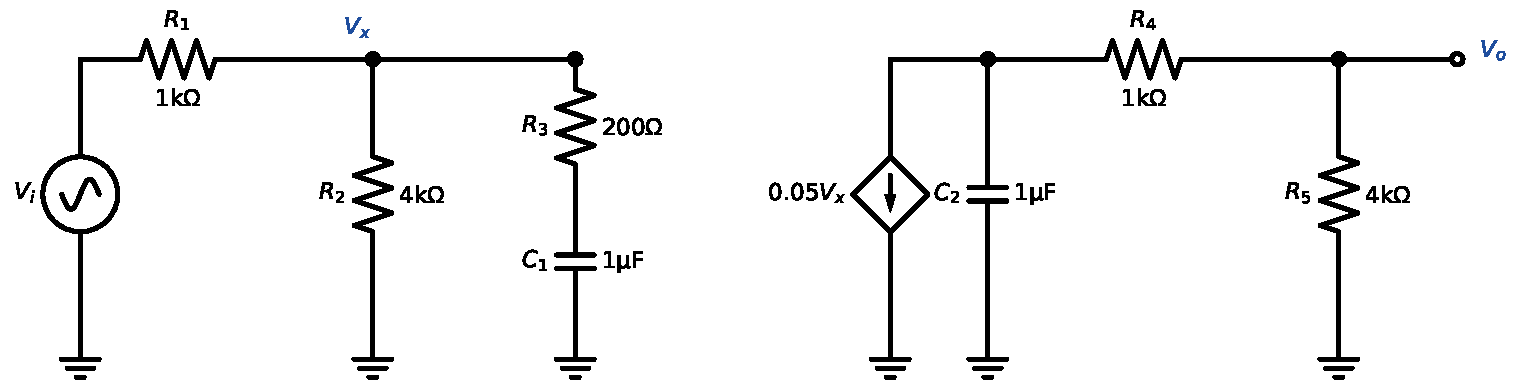
\includegraphics[width=\linewidth,height=5.5cm,keepaspectratio]{p14_circuit}\end{center}
\end{probbox}

\begin{probbox}{Problem 1C.15 \hfill Hard}
For the circuit below: (a) find the AC transfer function $H(s)=\dfrac{V_o(s)}{V_i(s)}$ and sketch its magnitude Bode plot; (b) find the steady-state output $V_o(t)$ for $V_i(t) = 0.1\sin\left(2\pi\cdot 2000\,t+\frac{\pi}{4}\right)$.
\begin{center}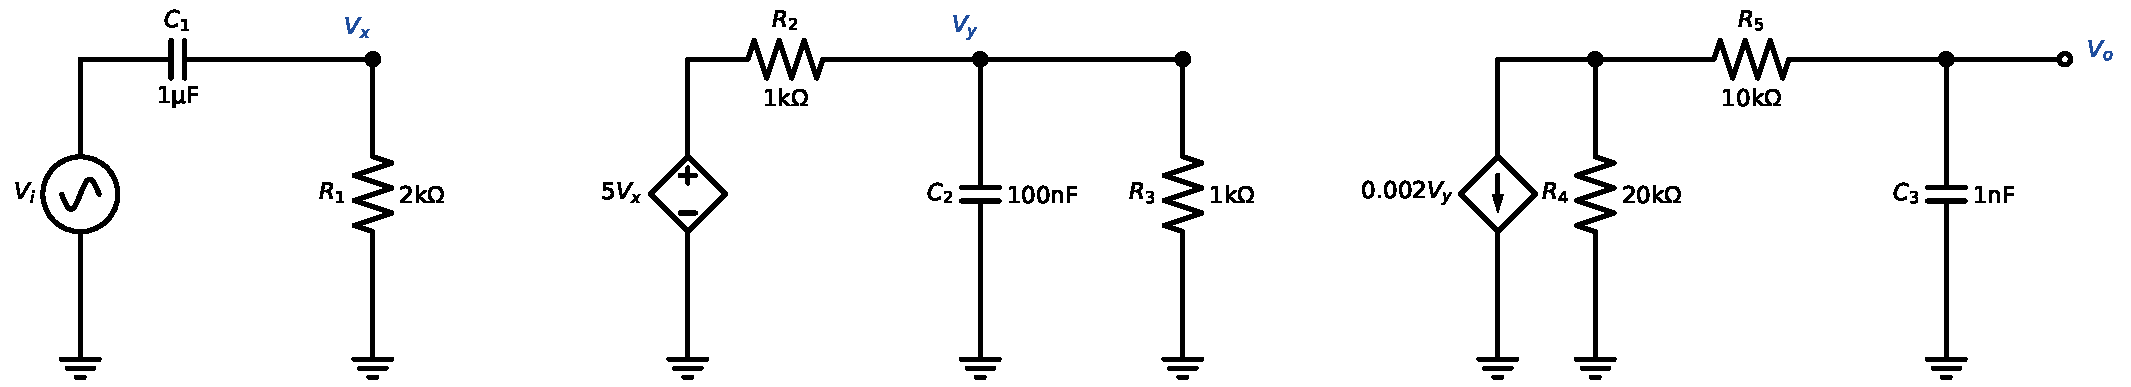
\includegraphics[width=\linewidth,height=5.5cm,keepaspectratio]{p15_circuit}\end{center}
\end{probbox}

\begin{probbox}{Problem 1C.16 \hfill Hard}
For the circuit below: (a) find the AC transfer function $H(s)=\dfrac{V_o(s)}{V_i(s)}$ and sketch its magnitude Bode plot; (b) find the steady-state output $V_o(t)$ for $V_i(t) = 0.1\cos\left(2\pi\cdot 3000\,t\right)$.
\begin{center}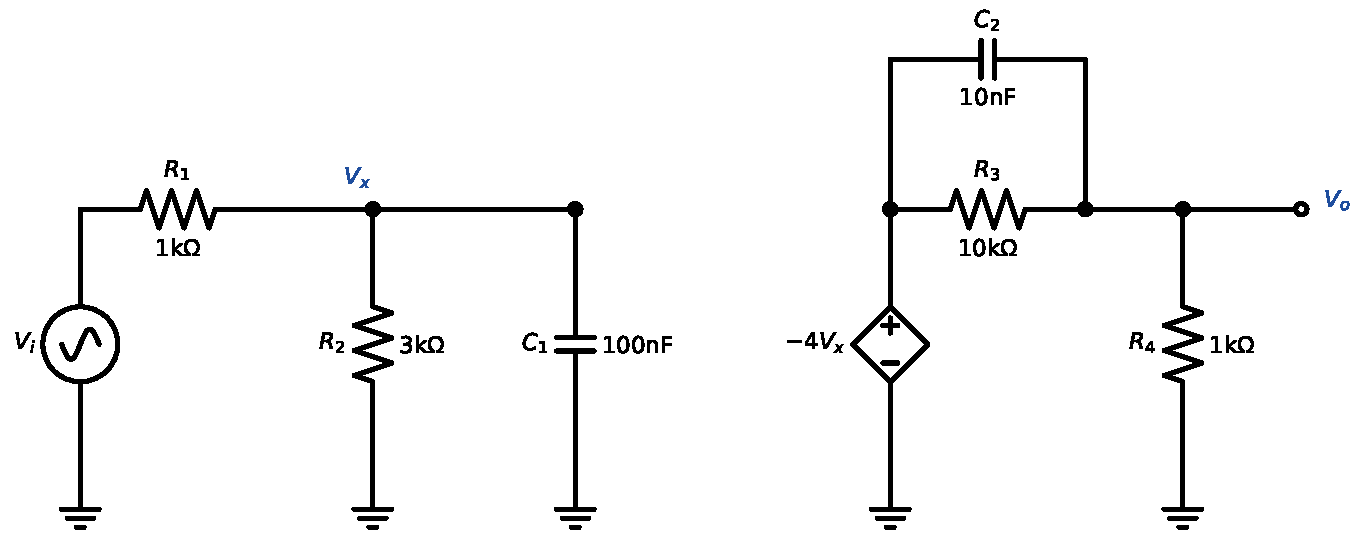
\includegraphics[width=\linewidth,height=5.5cm,keepaspectratio]{p16_circuit}\end{center}
\end{probbox}

\begin{probbox}{Problem 1C.17 \hfill Hard}
For the circuit below: (a) find the AC transfer function $H(s)=\dfrac{V_o(s)}{V_i(s)}$ and sketch its magnitude Bode plot; (b) find the steady-state output $V_o(t)$ for $V_i(t) = 0.2\sin\left(2\pi\cdot 5000\,t-\frac{\pi}{6}\right)$.
\begin{center}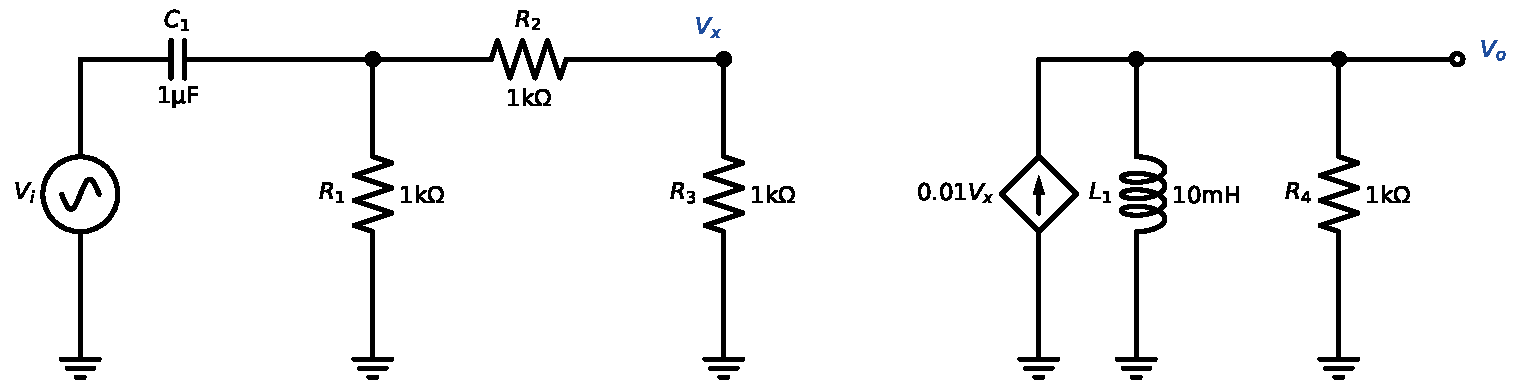
\includegraphics[width=\linewidth,height=5.5cm,keepaspectratio]{p17_circuit}\end{center}
\end{probbox}

\begin{probbox}{Problem 1C.18 \hfill Hard}
For the circuit below: (a) find the AC transfer function $H(s)=\dfrac{V_o(s)}{V_i(s)}$ and sketch its magnitude Bode plot; (b) find the steady-state output $V_o(t)$ for $V_i(t) = 0.01\cos\left(2\pi\cdot 500\,t+\frac{\pi}{3}\right)$.
\begin{center}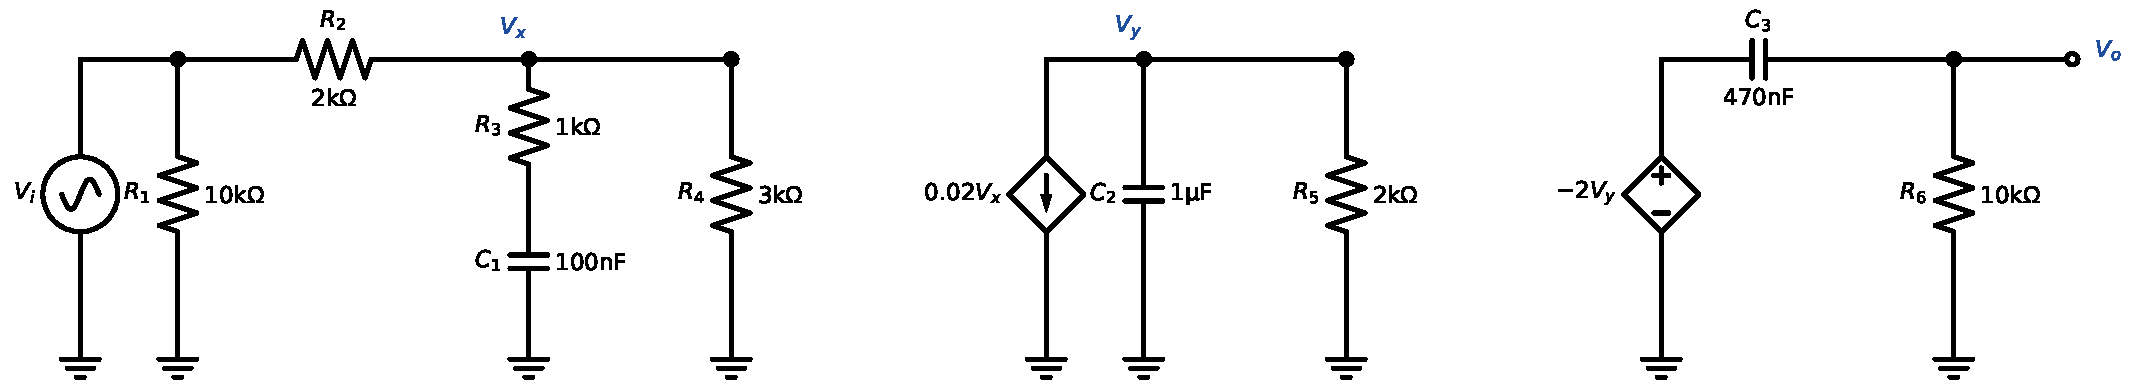
\includegraphics[width=\linewidth,height=5.5cm,keepaspectratio]{p18_circuit}\end{center}
\end{probbox}

\newpage
\section*{Solutions}
Every solution follows the same seven steps of the pipeline card.
\newpage
\subsection*{Solution 1C.1 \hfill Easy}
\begin{center}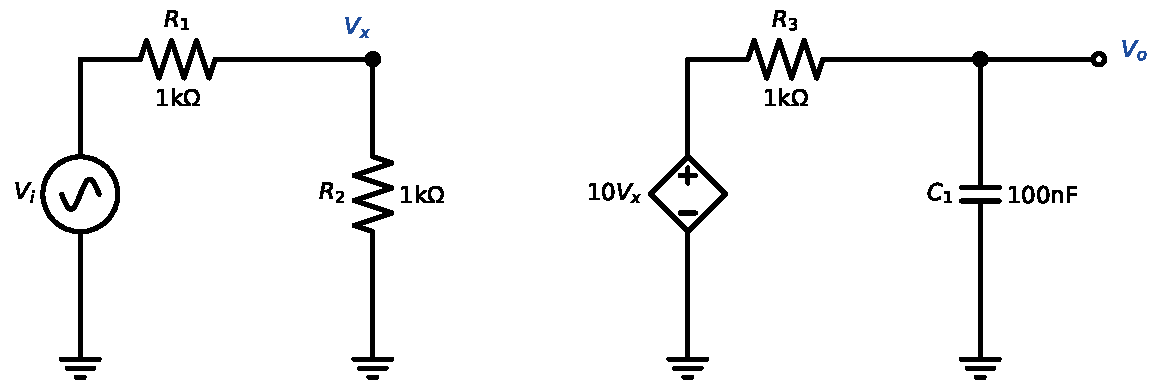
\includegraphics[width=0.8\linewidth,height=4.5cm,keepaspectratio]{p01_circuit}\end{center}
\solstep{1}{Identify the sources}Independent sources: the AC input $V_i(t)$. The diamond-shaped sources are \emph{dependent} sources: they are not inputs, they only copy/scale a voltage that already exists in the circuit, so they stay in the circuit in every step. There is no DC source, so $V_{o,dc}=0$ and $V_o(t)=v_{o,ac}(t)$: Step 2 is skipped.
\solstep{2}{DC circuit}No DC sources: $V_{o,dc}=0$.
\solstep{3}{AC circuit}Replace every capacitor by $\frac{1}{sC}$ and every inductor by $sL$.
AC equivalent circuit (nodes named for the next step):
\begin{center}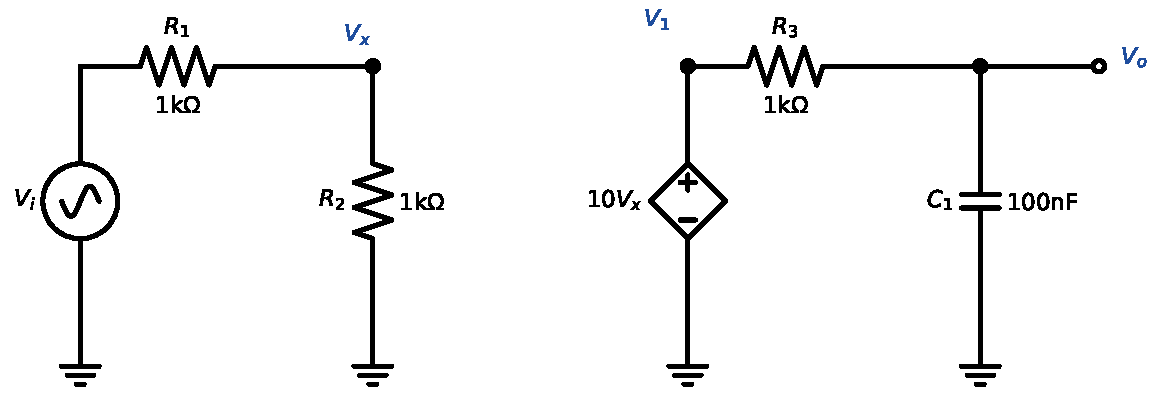
\includegraphics[width=0.95\linewidth,height=5.2cm,keepaspectratio]{p01_ac}\end{center}

\solstep{4}{Transfer function by a chain of dividers}Walk from the input to the output through the named nodes: $V_{i} \to V_{x} \to V_{1} \to V_{o}$. The transfer function is the product of the node-to-node ratios (each one is a simple divider, tool T2, or a dependent source, tool T4):
\[
H(s) = \frac{V_o}{V_i} = \frac{V_{x}}{V_{i}}\cdot\frac{V_{1}}{V_{x}}\cdot\frac{V_{o}}{V_{1}}
\]

Now each link. {\small (Algebra tip: to simplify a fraction that contains fractions, multiply its top and bottom by every inner denominator; then divide top and bottom by the leading coefficient of the denominator so that it starts with a plain $s^n$.)}
\begin{align*}
\frac{V_{x}}{V_{i}} &= \frac{R_{2}}{R_{1} + R_{2}} = 0.5 \\
\frac{V_{1}}{V_{x}} &= 10 &&\text{(ideal VCVS: $V_{1} = 10V_{x}$)} \\
\frac{V_{o}}{V_{1}} &= \frac{\frac{1}{sC_{1}}}{R_{3} + \frac{1}{sC_{1}}} = \dfrac{10000}{s + 10000}
\end{align*}

Multiply the links and simplify (common factors cancel):\[
H(s) = \dfrac{50000}{s + 10000}
\]

\solstep{5}{Standard (Bode-ready) form}Find the roots. Every root $s=-p$ of the denominator is a \emph{pole}, every root $s=-z$ of the numerator is a \emph{zero}; $|p|$ and $|z|$ are the corner frequencies (rad/s).
\begin{itemize}[leftmargin=*,itemsep=2pt]
\item Denominator: $s + 10000$; $s + 10000 = 0 \Rightarrow s = -10000$.
\end{itemize}

Factored form (leading coefficient in front):
\[
H(s) = 50000\,\dfrac{1}{(s+10000)}
\]

Bode-ready form: rewrite every $(s+p) = p\left(1+\frac{s}{p}\right)$ and $(s+z) = z\left(1+\frac{s}{z}\right)$, and collect all constants into $K$. Then every factor except $K$ is $\approx 1$ inside the pass-band:
\[
H(s) = 5\,\dfrac{1}{1+\dfrac{s}{2\pi\cdot 1.59\mathrm{k}}},\qquad K = 5
\]

\begin{center}\renewcommand{\arraystretch}{1.35}
\begin{tabular}{cccc}
\toprule
type & $\omega_c$ (rad/s) & $f_c=\omega_c/2\pi$ & slope change \\
\midrule
pole & $10000$ & 1.59 kHz & $-20$ dB/dec \\
\bottomrule
\end{tabular}\end{center}

\solstep{6}{Magnitude Bode plot}Below every corner, all factors are $\approx$ constant: $|H| \approx 5$ $= 14$\,dB (flat, 0 dB/dec). Then, moving right, each pole bends the line down by 20\,dB/dec and each zero bends it up by 20\,dB/dec (tool T6):
\begin{center}\renewcommand{\arraystretch}{1.35}
\begin{tabular}{lcl}
\toprule
frequency range & slope & asymptote level \\
\midrule
$f<$ 1.59 kHz & $0$ dB/dec (flat) & 14 dB at end \\
$f>$ 1.59 kHz & $-20$ dB/dec & 14 dB at start \\
\bottomrule
\end{tabular}\end{center}

The flat (pass-band) level is $20\log_{10}|K| = 20\log_{10}5 = 14$\,dB.
\begin{center}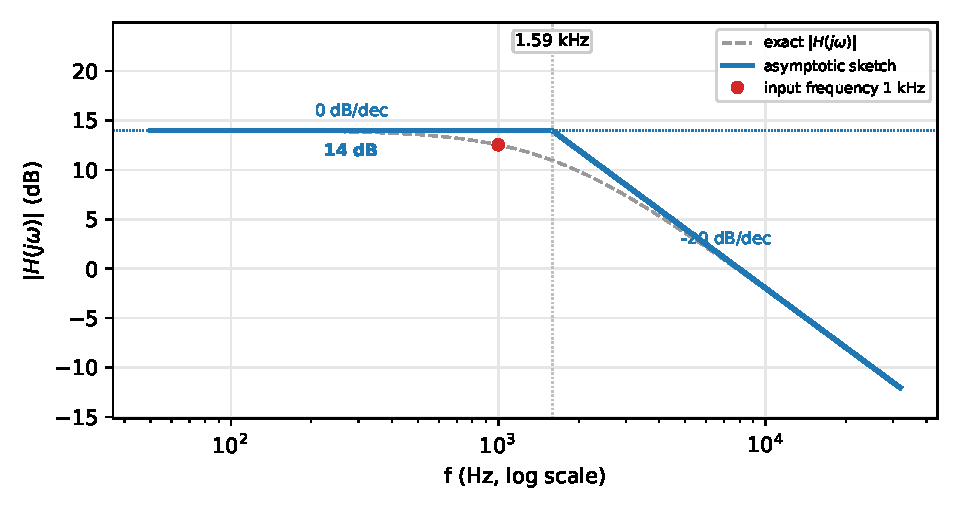
\includegraphics[width=0.78\linewidth,height=6.5cm,keepaspectratio]{p01_bode}\end{center}

{\small Blue: the straight-line sketch you are expected to draw. Dashed grey: the exact curve (about 3\,dB below the corner of an isolated pole). Red dot: the input frequency of Step 7.}
\solstep{7}{Steady-state output}The input is $V_i(t) = 0.1\sin\left(2\pi\cdot 1000\,t\right)$, so $\omega_{in} = 2\pi\cdot 1000 = 6280$\,rad/s. Put $s=j\omega_{in}$ in each factor (tool T5): magnitudes multiply, angles add.
{\small Rules: $\left|\frac{s}{s+p}\right| = \frac{\omega}{\sqrt{\omega^2+p^2}}$, $\angle = \frac{\pi}{2}-\tan^{-1}\frac{\omega}{p}$;\quad $\left|\frac{1}{1+s/p}\right| = \frac{1}{\sqrt{1+(\omega/p)^2}}$, $\angle = -\tan^{-1}\frac{\omega}{p}$;\quad $\left|1+\frac{s}{z}\right| = \sqrt{1+(\omega/z)^2}$, $\angle = \tan^{-1}\frac{\omega}{z}$;\quad a negative $K$ adds $-\pi$.}
\begin{center}\renewcommand{\arraystretch}{1.35}
\begin{tabular}{ccc}
\toprule
factor & magnitude & angle (rad) \\
\midrule
$5$ & $5$ & $0$ \\
$\rule[-1.7em]{0pt}{4em}\dfrac{1}{1+\dfrac{s}{2\pi\cdot 1.59\mathrm{k}}}$ & $0.8467$ & $-0.561$ \\
\textbf{total} & $\mathbf{4.234}$ (product) & $\mathbf{-0.561}$ (sum) \\
\bottomrule
\end{tabular}\end{center}

\begin{align*}
|H(j\omega_{in})| &= 4.23, \qquad \angle H(j\omega_{in}) = -0.561\ \mathrm{rad} \\
v_{o,ac}(t) &= 4.23\times 0.1\,\sin\left(2\pi\cdot 1000\,t - 0.561\right) = 0.423\,\sin\left(2\pi\cdot 1000\,t - 0.561\right)
\end{align*}

\[
\boxed{V_o(t) = 0.423\,\sin\left(2\pi\cdot 1000\,t - 0.561\right)\ \mathrm{V}}
\]

\begin{ansbox}
$H(s) = 5\,\dfrac{1}{1+\dfrac{s}{2\pi\cdot 1.59\mathrm{k}}}$\quad (corners: 1.59 kHz)\\[4pt]
$V_o(t) = 0.423\,\sin\left(2\pi\cdot 1000\,t - 0.561\right)\ \mathrm{V}$
\end{ansbox}

\newpage
\subsection*{Solution 1C.2 \hfill Easy}
\begin{center}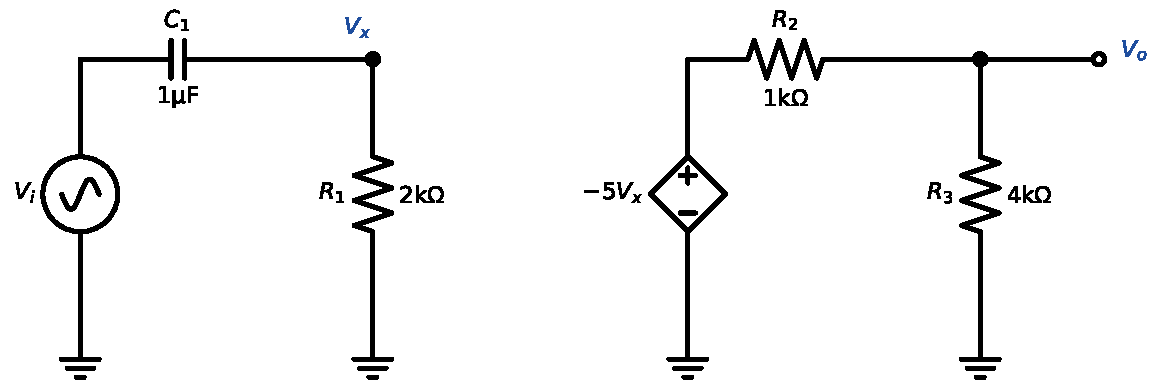
\includegraphics[width=0.8\linewidth,height=4.5cm,keepaspectratio]{p02_circuit}\end{center}
\solstep{1}{Identify the sources}Independent sources: the AC input $V_i(t)$. The diamond-shaped sources are \emph{dependent} sources: they are not inputs, they only copy/scale a voltage that already exists in the circuit, so they stay in the circuit in every step. There is no DC source, so $V_{o,dc}=0$ and $V_o(t)=v_{o,ac}(t)$: Step 2 is skipped.
\solstep{2}{DC circuit}No DC sources: $V_{o,dc}=0$.
\solstep{3}{AC circuit}Replace every capacitor by $\frac{1}{sC}$ and every inductor by $sL$.
AC equivalent circuit (nodes named for the next step):
\begin{center}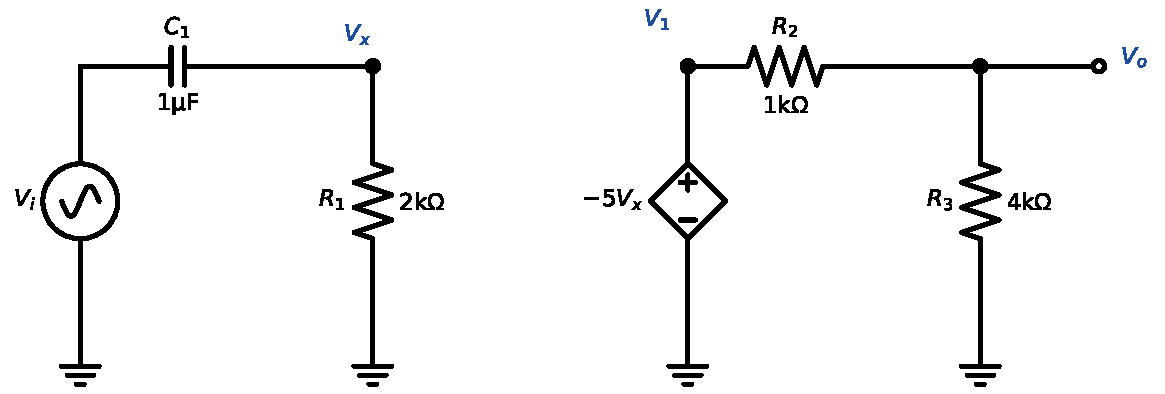
\includegraphics[width=0.95\linewidth,height=5.2cm,keepaspectratio]{p02_ac}\end{center}

\solstep{4}{Transfer function by a chain of dividers}Walk from the input to the output through the named nodes: $V_{i} \to V_{x} \to V_{1} \to V_{o}$. The transfer function is the product of the node-to-node ratios (each one is a simple divider, tool T2, or a dependent source, tool T4):
\[
H(s) = \frac{V_o}{V_i} = \frac{V_{x}}{V_{i}}\cdot\frac{V_{1}}{V_{x}}\cdot\frac{V_{o}}{V_{1}}
\]

Now each link. {\small (Algebra tip: to simplify a fraction that contains fractions, multiply its top and bottom by every inner denominator; then divide top and bottom by the leading coefficient of the denominator so that it starts with a plain $s^n$.)}
\begin{align*}
\frac{V_{x}}{V_{i}} &= \frac{R_{1}}{\frac{1}{sC_{1}} + R_{1}} = \dfrac{s}{s + 500} \\
\frac{V_{1}}{V_{x}} &= -5 &&\text{(ideal VCVS: $V_{1} = -5V_{x}$)} \\
\frac{V_{o}}{V_{1}} &= \frac{R_{3}}{R_{2} + R_{3}} = 0.8
\end{align*}

Multiply the links and simplify (common factors cancel):\[
H(s) = \dfrac{-4\,s}{s + 500}
\]

\solstep{5}{Standard (Bode-ready) form}Find the roots. Every root $s=-p$ of the denominator is a \emph{pole}, every root $s=-z$ of the numerator is a \emph{zero}; $|p|$ and $|z|$ are the corner frequencies (rad/s).
\begin{itemize}[leftmargin=*,itemsep=2pt]
\item Numerator: it has the factor $s$ $\Rightarrow$ 1 zero at $s=0$.
\item Denominator: $s + 500$; $s + 500 = 0 \Rightarrow s = -500$.
\end{itemize}

Factored form (leading coefficient in front):
\[
H(s) = -4\,\dfrac{s}{(s+500)}
\]

Bode-ready form: rewrite every $(s+p) = p\left(1+\frac{s}{p}\right)$ and $(s+z) = z\left(1+\frac{s}{z}\right)$, and collect all constants into $K$. Each $s$ in the numerator is paired with one of the \emph{lowest} poles as $\frac{s}{s+p}$ (that factor is $\approx 1$ above $p$). Then every factor except $K$ is $\approx 1$ inside the pass-band:
\[
H(s) = -4\,\dfrac{s}{s+2\pi\cdot 79.6},\qquad K = -4
\]

\begin{center}\renewcommand{\arraystretch}{1.35}
\begin{tabular}{cccc}
\toprule
type & $\omega_c$ (rad/s) & $f_c=\omega_c/2\pi$ & slope change \\
\midrule
pole & $500$ & 79.6 Hz & $-20$ dB/dec \\
\bottomrule
\end{tabular}\end{center}

\solstep{6}{Magnitude Bode plot}Below every corner $|H(s)|\approx 0.008\,s$, so the plot starts with a slope of $+20$\,dB/dec. Then, moving right, each pole bends the line down by 20\,dB/dec and each zero bends it up by 20\,dB/dec (tool T6):
\begin{center}\renewcommand{\arraystretch}{1.35}
\begin{tabular}{lcl}
\toprule
frequency range & slope & asymptote level \\
\midrule
$f<$ 79.6 Hz & $+20$ dB/dec & 12 dB at end \\
$f>$ 79.6 Hz & $0$ dB/dec (flat) & 12 dB at start \\
\bottomrule
\end{tabular}\end{center}

The flat (pass-band) level is $20\log_{10}|K| = 20\log_{10}4 = 12$\,dB.
\begin{center}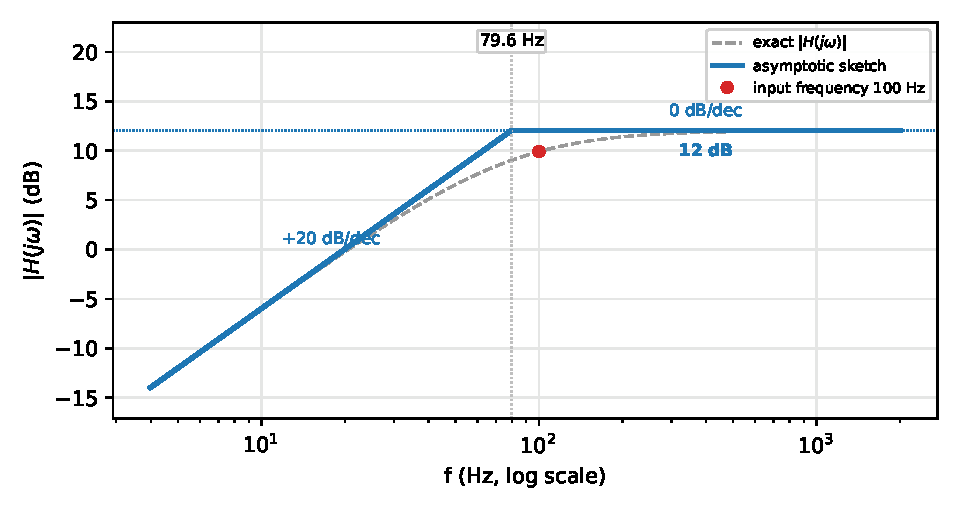
\includegraphics[width=0.78\linewidth,height=6.5cm,keepaspectratio]{p02_bode}\end{center}

{\small Blue: the straight-line sketch you are expected to draw. Dashed grey: the exact curve (about 3\,dB below the corner of an isolated pole). Red dot: the input frequency of Step 7.}
\solstep{7}{Steady-state output}The input is $V_i(t) = 0.2\sin\left(2\pi\cdot 100\,t\right)$, so $\omega_{in} = 2\pi\cdot 100 = 628$\,rad/s. Put $s=j\omega_{in}$ in each factor (tool T5): magnitudes multiply, angles add.
{\small Rules: $\left|\frac{s}{s+p}\right| = \frac{\omega}{\sqrt{\omega^2+p^2}}$, $\angle = \frac{\pi}{2}-\tan^{-1}\frac{\omega}{p}$;\quad $\left|\frac{1}{1+s/p}\right| = \frac{1}{\sqrt{1+(\omega/p)^2}}$, $\angle = -\tan^{-1}\frac{\omega}{p}$;\quad $\left|1+\frac{s}{z}\right| = \sqrt{1+(\omega/z)^2}$, $\angle = \tan^{-1}\frac{\omega}{z}$;\quad a negative $K$ adds $-\pi$.}
\begin{center}\renewcommand{\arraystretch}{1.35}
\begin{tabular}{ccc}
\toprule
factor & magnitude & angle (rad) \\
\midrule
$-4$ & $4$ & $-3.14$ \\
$\rule[-1.1em]{0pt}{2.8em}\dfrac{s}{s+2\pi\cdot 79.6}$ & $0.7825$ & $0.672$ \\
\textbf{total} & $\mathbf{3.13}$ (product) & $\mathbf{-2.47}$ (sum) \\
\bottomrule
\end{tabular}\end{center}

\begin{align*}
|H(j\omega_{in})| &= 3.13, \qquad \angle H(j\omega_{in}) = -2.47\ \mathrm{rad} \\
v_{o,ac}(t) &= 3.13\times 0.2\,\sin\left(2\pi\cdot 100\,t - 2.47\right) = 0.626\,\sin\left(2\pi\cdot 100\,t - 2.47\right)
\end{align*}

\[
\boxed{V_o(t) = 0.626\,\sin\left(2\pi\cdot 100\,t - 2.47\right)\ \mathrm{V}}
\]

\begin{ansbox}
$H(s) = -4\,\dfrac{s}{s+2\pi\cdot 79.6}$\quad (corners: 79.6 Hz)\\[4pt]
$V_o(t) = 0.626\,\sin\left(2\pi\cdot 100\,t - 2.47\right)\ \mathrm{V}$
\end{ansbox}

\newpage
\subsection*{Solution 1C.3 \hfill Easy}
\begin{center}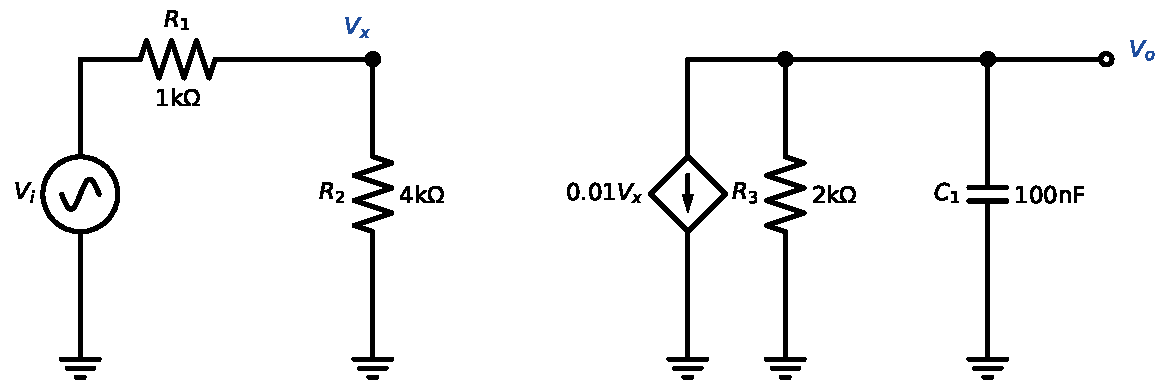
\includegraphics[width=0.8\linewidth,height=4.5cm,keepaspectratio]{p03_circuit}\end{center}
\solstep{1}{Identify the sources}Independent sources: the AC input $V_i(t)$. The diamond-shaped sources are \emph{dependent} sources: they are not inputs, they only copy/scale a voltage that already exists in the circuit, so they stay in the circuit in every step. There is no DC source, so $V_{o,dc}=0$ and $V_o(t)=v_{o,ac}(t)$: Step 2 is skipped.
\solstep{2}{DC circuit}No DC sources: $V_{o,dc}=0$.
\solstep{3}{AC circuit}Replace every capacitor by $\frac{1}{sC}$ and every inductor by $sL$.
AC equivalent circuit (nodes named for the next step):
\begin{center}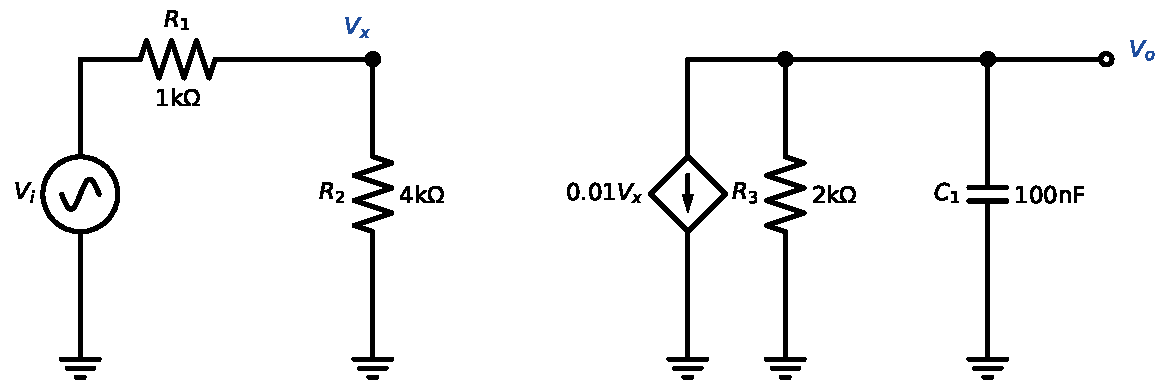
\includegraphics[width=0.95\linewidth,height=5.2cm,keepaspectratio]{p03_ac}\end{center}

\solstep{4}{Transfer function by a chain of dividers}Walk from the input to the output through the named nodes: $V_{i} \to V_{x} \to V_{o}$. The transfer function is the product of the node-to-node ratios (each one is a simple divider, tool T2, or a dependent source, tool T4):
\[
H(s) = \frac{V_o}{V_i} = \frac{V_{x}}{V_{i}}\cdot\frac{V_{o}}{V_{x}}
\]

Impedances seen \emph{looking right} from a node (everything from that node to ground, excluding what is on its left). Compute them from the far right toward the input:
\begin{align*}
Z_{o} &= R_{3} \parallel \frac{1}{sC_{1}} = \dfrac{10^{7}}{s + 5000}
\end{align*}

Now each link. {\small (Algebra tip: to simplify a fraction that contains fractions, multiply its top and bottom by every inner denominator; then divide top and bottom by the leading coefficient of the denominator so that it starts with a plain $s^n$.)}
\begin{align*}
\frac{V_{x}}{V_{i}} &= \frac{R_{2}}{R_{1} + R_{2}} = 0.8 \\
\frac{V_{o}}{V_{x}} &= -0.01\,Z_{o} = \dfrac{-10^{5}}{s + 5000}
\end{align*}

(VCCS: the current $0.01V_{x}$ flows out of node $V_{o}$ and through $Z_{o}$ to ground, so $V_{o} = -0.01V_{x}\,Z_{o}$ by Ohm's law.)
Multiply the links and simplify (common factors cancel):\[
H(s) = \dfrac{-80000}{s + 5000}
\]

\solstep{5}{Standard (Bode-ready) form}Find the roots. Every root $s=-p$ of the denominator is a \emph{pole}, every root $s=-z$ of the numerator is a \emph{zero}; $|p|$ and $|z|$ are the corner frequencies (rad/s).
\begin{itemize}[leftmargin=*,itemsep=2pt]
\item Denominator: $s + 5000$; $s + 5000 = 0 \Rightarrow s = -5000$.
\end{itemize}

Factored form (leading coefficient in front):
\[
H(s) = -80000\,\dfrac{1}{(s+5000)}
\]

Bode-ready form: rewrite every $(s+p) = p\left(1+\frac{s}{p}\right)$ and $(s+z) = z\left(1+\frac{s}{z}\right)$, and collect all constants into $K$. Then every factor except $K$ is $\approx 1$ inside the pass-band:
\[
H(s) = -16\,\dfrac{1}{1+\dfrac{s}{2\pi\cdot 796}},\qquad K = -16
\]

\begin{center}\renewcommand{\arraystretch}{1.35}
\begin{tabular}{cccc}
\toprule
type & $\omega_c$ (rad/s) & $f_c=\omega_c/2\pi$ & slope change \\
\midrule
pole & $5000$ & 796 Hz & $-20$ dB/dec \\
\bottomrule
\end{tabular}\end{center}

\solstep{6}{Magnitude Bode plot}Below every corner, all factors are $\approx$ constant: $|H| \approx 16$ $= 24.1$\,dB (flat, 0 dB/dec). Then, moving right, each pole bends the line down by 20\,dB/dec and each zero bends it up by 20\,dB/dec (tool T6):
\begin{center}\renewcommand{\arraystretch}{1.35}
\begin{tabular}{lcl}
\toprule
frequency range & slope & asymptote level \\
\midrule
$f<$ 796 Hz & $0$ dB/dec (flat) & 24.1 dB at end \\
$f>$ 796 Hz & $-20$ dB/dec & 24.1 dB at start \\
\bottomrule
\end{tabular}\end{center}

The flat (pass-band) level is $20\log_{10}|K| = 20\log_{10}16 = 24.1$\,dB.
\begin{center}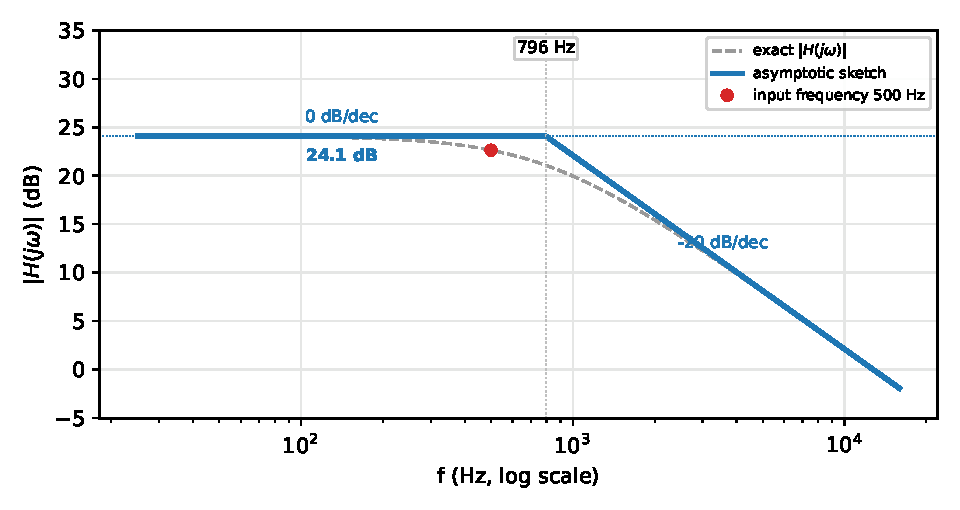
\includegraphics[width=0.78\linewidth,height=6.5cm,keepaspectratio]{p03_bode}\end{center}

{\small Blue: the straight-line sketch you are expected to draw. Dashed grey: the exact curve (about 3\,dB below the corner of an isolated pole). Red dot: the input frequency of Step 7.}
\solstep{7}{Steady-state output}The input is $V_i(t) = 0.05\sin\left(2\pi\cdot 500\,t\right)$, so $\omega_{in} = 2\pi\cdot 500 = 3140$\,rad/s. Put $s=j\omega_{in}$ in each factor (tool T5): magnitudes multiply, angles add.
{\small Rules: $\left|\frac{s}{s+p}\right| = \frac{\omega}{\sqrt{\omega^2+p^2}}$, $\angle = \frac{\pi}{2}-\tan^{-1}\frac{\omega}{p}$;\quad $\left|\frac{1}{1+s/p}\right| = \frac{1}{\sqrt{1+(\omega/p)^2}}$, $\angle = -\tan^{-1}\frac{\omega}{p}$;\quad $\left|1+\frac{s}{z}\right| = \sqrt{1+(\omega/z)^2}$, $\angle = \tan^{-1}\frac{\omega}{z}$;\quad a negative $K$ adds $-\pi$.}
\begin{center}\renewcommand{\arraystretch}{1.35}
\begin{tabular}{ccc}
\toprule
factor & magnitude & angle (rad) \\
\midrule
$-16$ & $16$ & $-3.14$ \\
$\rule[-1.7em]{0pt}{4em}\dfrac{1}{1+\dfrac{s}{2\pi\cdot 796}}$ & $0.8467$ & $-0.561$ \\
\textbf{total} & $\mathbf{13.55}$ (product) & $\mathbf{-3.7}$ (sum) \\
\bottomrule
\end{tabular}\end{center}

\begin{align*}
|H(j\omega_{in})| &= 13.5, \qquad \angle H(j\omega_{in}) = -3.7\ \mathrm{rad} \\
v_{o,ac}(t) &= 13.5\times 0.05\,\sin\left(2\pi\cdot 500\,t - 3.7\right) = 0.677\,\sin\left(2\pi\cdot 500\,t - 3.7\right)
\end{align*}

\[
\boxed{V_o(t) = 0.677\,\sin\left(2\pi\cdot 500\,t - 3.7\right)\ \mathrm{V}}
\]

\begin{ansbox}
$H(s) = -16\,\dfrac{1}{1+\dfrac{s}{2\pi\cdot 796}}$\quad (corners: 796 Hz)\\[4pt]
$V_o(t) = 0.677\,\sin\left(2\pi\cdot 500\,t - 3.7\right)\ \mathrm{V}$
\end{ansbox}

\newpage
\subsection*{Solution 1C.4 \hfill Easy}
\begin{center}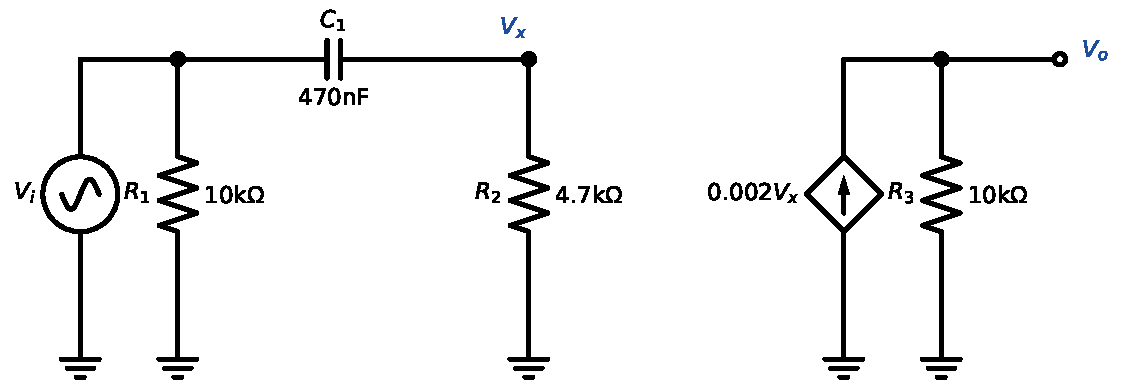
\includegraphics[width=0.8\linewidth,height=4.5cm,keepaspectratio]{p04_circuit}\end{center}
\solstep{1}{Identify the sources}Independent sources: the AC input $V_i(t)$. The diamond-shaped sources are \emph{dependent} sources: they are not inputs, they only copy/scale a voltage that already exists in the circuit, so they stay in the circuit in every step. There is no DC source, so $V_{o,dc}=0$ and $V_o(t)=v_{o,ac}(t)$: Step 2 is skipped.
\solstep{2}{DC circuit}No DC sources: $V_{o,dc}=0$.
\solstep{3}{AC circuit}Replace every capacitor by $\frac{1}{sC}$ and every inductor by $sL$.
\begin{itemize}[leftmargin=*,itemsep=2pt]
\item $R_{1}$ sits directly across the ideal input source $V_i$. An ideal voltage source keeps its voltage whatever you connect to it, so $R_{1}$ cannot change any node voltage: it drops out of $H(s)$.
\end{itemize}

AC equivalent circuit (nodes named for the next step):
\begin{center}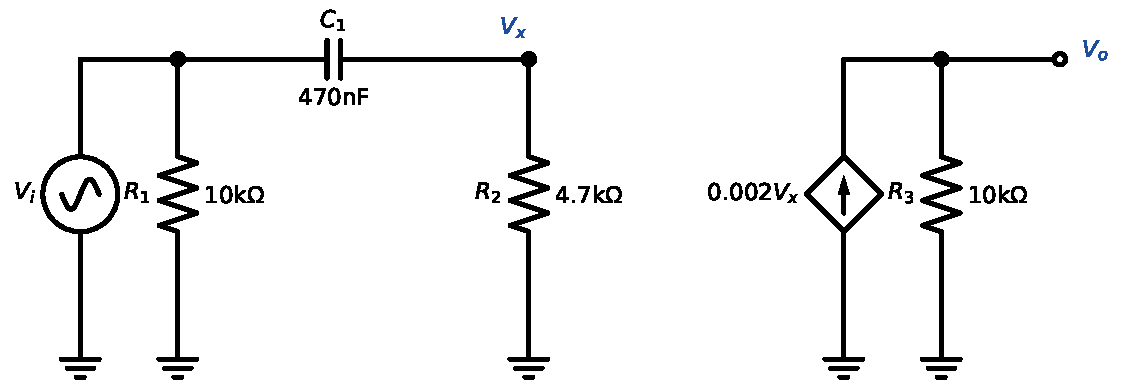
\includegraphics[width=0.95\linewidth,height=5.2cm,keepaspectratio]{p04_ac}\end{center}

\solstep{4}{Transfer function by a chain of dividers}Walk from the input to the output through the named nodes: $V_{i} \to V_{x} \to V_{o}$. The transfer function is the product of the node-to-node ratios (each one is a simple divider, tool T2, or a dependent source, tool T4):
\[
H(s) = \frac{V_o}{V_i} = \frac{V_{x}}{V_{i}}\cdot\frac{V_{o}}{V_{x}}
\]

Now each link. {\small (Algebra tip: to simplify a fraction that contains fractions, multiply its top and bottom by every inner denominator; then divide top and bottom by the leading coefficient of the denominator so that it starts with a plain $s^n$.)}
\begin{align*}
\frac{V_{x}}{V_{i}} &= \frac{R_{2}}{\frac{1}{sC_{1}} + R_{2}} = \dfrac{s}{s + 453} \\
\frac{V_{o}}{V_{x}} &= 0.002\,R_{3} = 20
\end{align*}

(VCCS: the current $0.002V_{x}$ flows into node $V_{o}$ and through $R_{3}$ to ground, so $V_{o} = 0.002V_{x}\,R_{3}$ by Ohm's law.)
Multiply the links and simplify (common factors cancel):\[
H(s) = \dfrac{20\,s}{s + 453}
\]

\solstep{5}{Standard (Bode-ready) form}Find the roots. Every root $s=-p$ of the denominator is a \emph{pole}, every root $s=-z$ of the numerator is a \emph{zero}; $|p|$ and $|z|$ are the corner frequencies (rad/s).
\begin{itemize}[leftmargin=*,itemsep=2pt]
\item Numerator: it has the factor $s$ $\Rightarrow$ 1 zero at $s=0$.
\item Denominator: $s + 453$; $s + 453 = 0 \Rightarrow s = -453$.
\end{itemize}

Factored form (leading coefficient in front):
\[
H(s) = 20\,\dfrac{s}{(s+453)}
\]

Bode-ready form: rewrite every $(s+p) = p\left(1+\frac{s}{p}\right)$ and $(s+z) = z\left(1+\frac{s}{z}\right)$, and collect all constants into $K$. Each $s$ in the numerator is paired with one of the \emph{lowest} poles as $\frac{s}{s+p}$ (that factor is $\approx 1$ above $p$). Then every factor except $K$ is $\approx 1$ inside the pass-band:
\[
H(s) = 20\,\dfrac{s}{s+2\pi\cdot 72},\qquad K = 20
\]

\begin{center}\renewcommand{\arraystretch}{1.35}
\begin{tabular}{cccc}
\toprule
type & $\omega_c$ (rad/s) & $f_c=\omega_c/2\pi$ & slope change \\
\midrule
pole & $453$ & 72 Hz & $-20$ dB/dec \\
\bottomrule
\end{tabular}\end{center}

\solstep{6}{Magnitude Bode plot}Below every corner $|H(s)|\approx 0.0442\,s$, so the plot starts with a slope of $+20$\,dB/dec. Then, moving right, each pole bends the line down by 20\,dB/dec and each zero bends it up by 20\,dB/dec (tool T6):
\begin{center}\renewcommand{\arraystretch}{1.35}
\begin{tabular}{lcl}
\toprule
frequency range & slope & asymptote level \\
\midrule
$f<$ 72 Hz & $+20$ dB/dec & 26 dB at end \\
$f>$ 72 Hz & $0$ dB/dec (flat) & 26 dB at start \\
\bottomrule
\end{tabular}\end{center}

The flat (pass-band) level is $20\log_{10}|K| = 20\log_{10}20 = 26$\,dB.
\begin{center}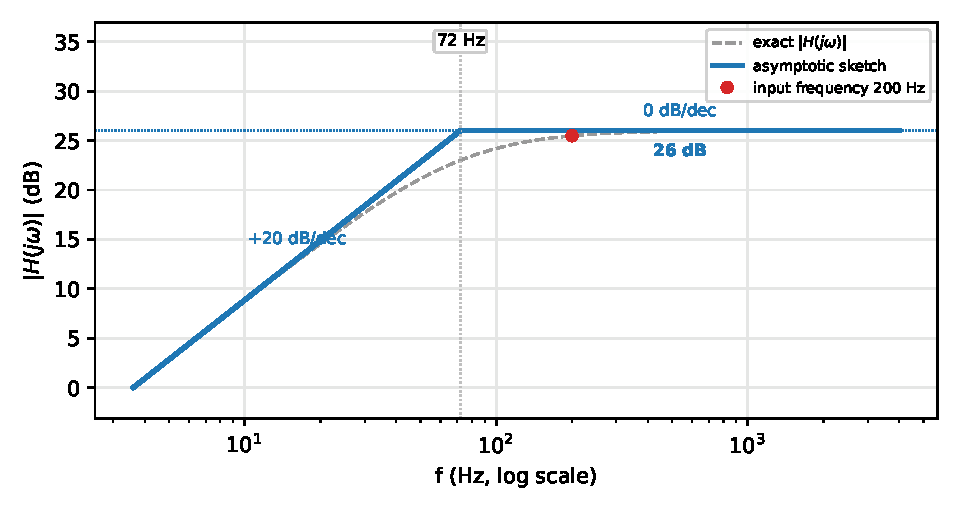
\includegraphics[width=0.78\linewidth,height=6.5cm,keepaspectratio]{p04_bode}\end{center}

{\small Blue: the straight-line sketch you are expected to draw. Dashed grey: the exact curve (about 3\,dB below the corner of an isolated pole). Red dot: the input frequency of Step 7.}
\solstep{7}{Steady-state output}The input is $V_i(t) = 0.1\sin\left(2\pi\cdot 200\,t\right)$, so $\omega_{in} = 2\pi\cdot 200 = 1260$\,rad/s. Put $s=j\omega_{in}$ in each factor (tool T5): magnitudes multiply, angles add.
{\small Rules: $\left|\frac{s}{s+p}\right| = \frac{\omega}{\sqrt{\omega^2+p^2}}$, $\angle = \frac{\pi}{2}-\tan^{-1}\frac{\omega}{p}$;\quad $\left|\frac{1}{1+s/p}\right| = \frac{1}{\sqrt{1+(\omega/p)^2}}$, $\angle = -\tan^{-1}\frac{\omega}{p}$;\quad $\left|1+\frac{s}{z}\right| = \sqrt{1+(\omega/z)^2}$, $\angle = \tan^{-1}\frac{\omega}{z}$;\quad a negative $K$ adds $-\pi$.}
\begin{center}\renewcommand{\arraystretch}{1.35}
\begin{tabular}{ccc}
\toprule
factor & magnitude & angle (rad) \\
\midrule
$20$ & $20$ & $0$ \\
$\rule[-1.1em]{0pt}{2.8em}\dfrac{s}{s+2\pi\cdot 72}$ & $0.9408$ & $0.346$ \\
\textbf{total} & $\mathbf{18.82}$ (product) & $\mathbf{0.346}$ (sum) \\
\bottomrule
\end{tabular}\end{center}

\begin{align*}
|H(j\omega_{in})| &= 18.8, \qquad \angle H(j\omega_{in}) = 0.346\ \mathrm{rad} \\
v_{o,ac}(t) &= 18.8\times 0.1\,\sin\left(2\pi\cdot 200\,t + 0.346\right) = 1.88\,\sin\left(2\pi\cdot 200\,t + 0.346\right)
\end{align*}

\[
\boxed{V_o(t) = 1.88\,\sin\left(2\pi\cdot 200\,t + 0.346\right)\ \mathrm{V}}
\]

\begin{ansbox}
$H(s) = 20\,\dfrac{s}{s+2\pi\cdot 72}$\quad (corners: 72 Hz)\\[4pt]
$V_o(t) = 1.88\,\sin\left(2\pi\cdot 200\,t + 0.346\right)\ \mathrm{V}$
\end{ansbox}

\newpage
\subsection*{Solution 1C.5 \hfill Easy}
\begin{center}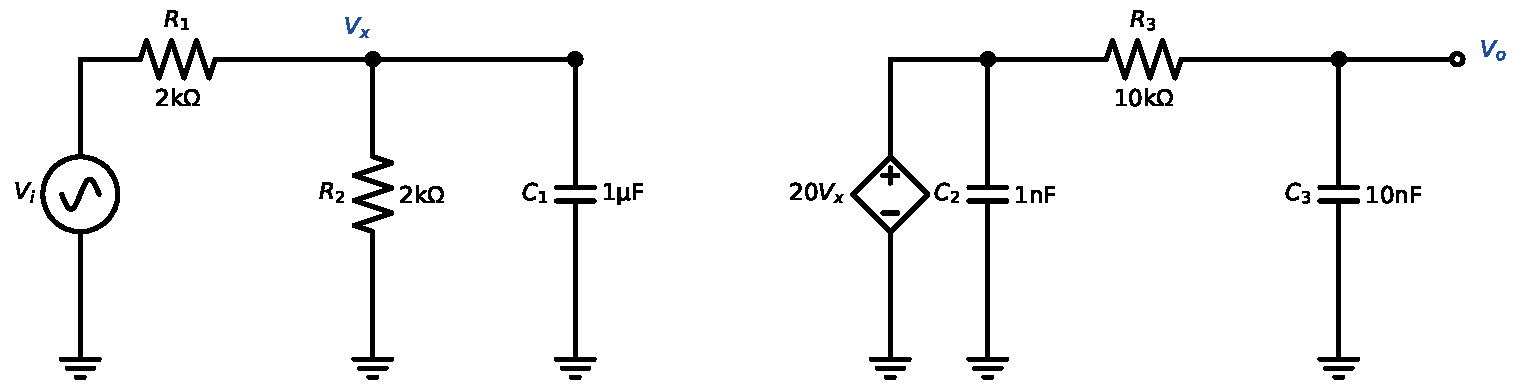
\includegraphics[width=0.8\linewidth,height=4.5cm,keepaspectratio]{p05_circuit}\end{center}
\solstep{1}{Identify the sources}Independent sources: the AC input $V_i(t)$. The diamond-shaped sources are \emph{dependent} sources: they are not inputs, they only copy/scale a voltage that already exists in the circuit, so they stay in the circuit in every step. There is no DC source, so $V_{o,dc}=0$ and $V_o(t)=v_{o,ac}(t)$: Step 2 is skipped.
\solstep{2}{DC circuit}No DC sources: $V_{o,dc}=0$.
\solstep{3}{AC circuit}Replace every capacitor by $\frac{1}{sC}$ and every inductor by $sL$.
\begin{itemize}[leftmargin=*,itemsep=2pt]
\item $C_{2}$ sits directly across the output of the ideal dependent voltage source. An ideal voltage source keeps its voltage whatever you connect to it, so $C_{2}$ cannot change any node voltage: it drops out of $H(s)$.
\end{itemize}

AC equivalent circuit (nodes named for the next step):
\begin{center}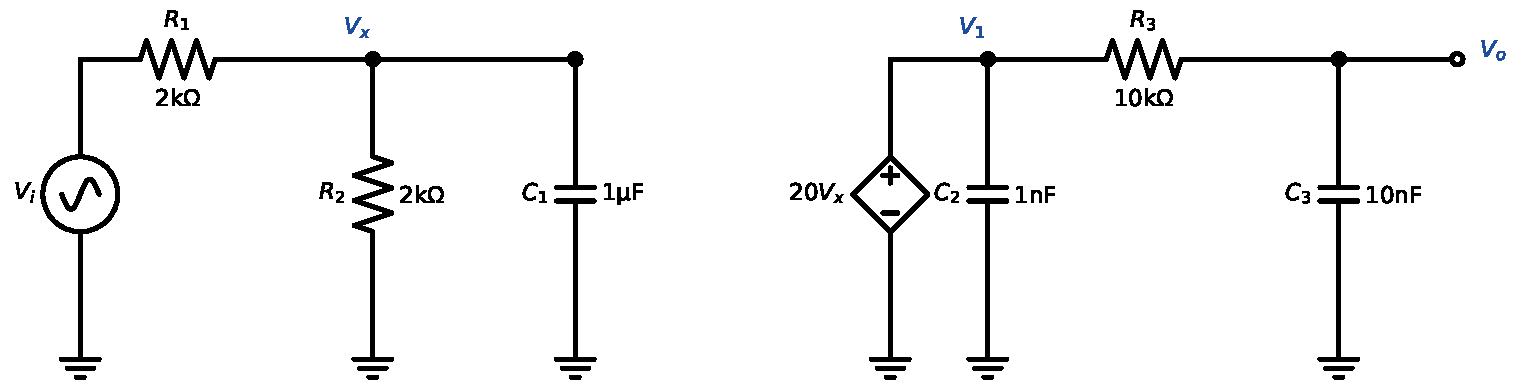
\includegraphics[width=0.95\linewidth,height=5.2cm,keepaspectratio]{p05_ac}\end{center}

\solstep{4}{Transfer function by a chain of dividers}Walk from the input to the output through the named nodes: $V_{i} \to V_{x} \to V_{1} \to V_{o}$. The transfer function is the product of the node-to-node ratios (each one is a simple divider, tool T2, or a dependent source, tool T4):
\[
H(s) = \frac{V_o}{V_i} = \frac{V_{x}}{V_{i}}\cdot\frac{V_{1}}{V_{x}}\cdot\frac{V_{o}}{V_{1}}
\]

Impedances seen \emph{looking right} from a node (everything from that node to ground, excluding what is on its left). Compute them from the far right toward the input:
\begin{align*}
Z_{x} &= R_{2} \parallel \frac{1}{sC_{1}} = \dfrac{10^{6}}{s + 500}
\end{align*}

Now each link. {\small (Algebra tip: to simplify a fraction that contains fractions, multiply its top and bottom by every inner denominator; then divide top and bottom by the leading coefficient of the denominator so that it starts with a plain $s^n$.)}
\begin{align*}
\frac{V_{x}}{V_{i}} &= \frac{Z_{x}}{R_{1} + Z_{x}} = \dfrac{500}{s + 1000} \\
\frac{V_{1}}{V_{x}} &= 20 &&\text{(ideal VCVS: $V_{1} = 20V_{x}$)} \\
\frac{V_{o}}{V_{1}} &= \frac{\frac{1}{sC_{3}}}{R_{3} + \frac{1}{sC_{3}}} = \dfrac{10000}{s + 10000}
\end{align*}

Multiply the links and simplify (common factors cancel):\[
H(s) = \dfrac{10^{8}}{s^{2} + 11000\,s + 10^{7}}
\]

\solstep{5}{Standard (Bode-ready) form}Find the roots. Every root $s=-p$ of the denominator is a \emph{pole}, every root $s=-z$ of the numerator is a \emph{zero}; $|p|$ and $|z|$ are the corner frequencies (rad/s).
\begin{itemize}[leftmargin=*,itemsep=2pt]
\item Denominator: $s^{2} + 11000\,s + 10^{7}$; quadratic formula:\[
s = \frac{-11000 \pm \sqrt{(11000)^2 - 4(10^{7})}}{2} = \frac{-11000 \pm 9000}{2} \Rightarrow s = -1000,\ -10000
\]

\end{itemize}

Factored form (leading coefficient in front):
\[
H(s) = 10^{8}\,\dfrac{1}{(s+1000)(s+10000)}
\]

Bode-ready form: rewrite every $(s+p) = p\left(1+\frac{s}{p}\right)$ and $(s+z) = z\left(1+\frac{s}{z}\right)$, and collect all constants into $K$. Then every factor except $K$ is $\approx 1$ inside the pass-band:
\[
H(s) = 10\,\dfrac{1}{1+\dfrac{s}{2\pi\cdot 159}}\,\dfrac{1}{1+\dfrac{s}{2\pi\cdot 1.59\mathrm{k}}},\qquad K = 10
\]

\begin{center}\renewcommand{\arraystretch}{1.35}
\begin{tabular}{cccc}
\toprule
type & $\omega_c$ (rad/s) & $f_c=\omega_c/2\pi$ & slope change \\
\midrule
pole & $1000$ & 159 Hz & $-20$ dB/dec \\
pole & $10000$ & 1.59 kHz & $-20$ dB/dec \\
\bottomrule
\end{tabular}\end{center}

\solstep{6}{Magnitude Bode plot}Below every corner, all factors are $\approx$ constant: $|H| \approx 10$ $= 20$\,dB (flat, 0 dB/dec). Then, moving right, each pole bends the line down by 20\,dB/dec and each zero bends it up by 20\,dB/dec (tool T6):
\begin{center}\renewcommand{\arraystretch}{1.35}
\begin{tabular}{lcl}
\toprule
frequency range & slope & asymptote level \\
\midrule
$f<$ 159 Hz & $0$ dB/dec (flat) & 20 dB at end \\
159 Hz -- 1.59 kHz & $-20$ dB/dec & 20 dB at start, 0 dB at end \\
$f>$ 1.59 kHz & $-40$ dB/dec & 0 dB at start \\
\bottomrule
\end{tabular}\end{center}

The flat (pass-band) level is $20\log_{10}|K| = 20\log_{10}10 = 20$\,dB.
\begin{center}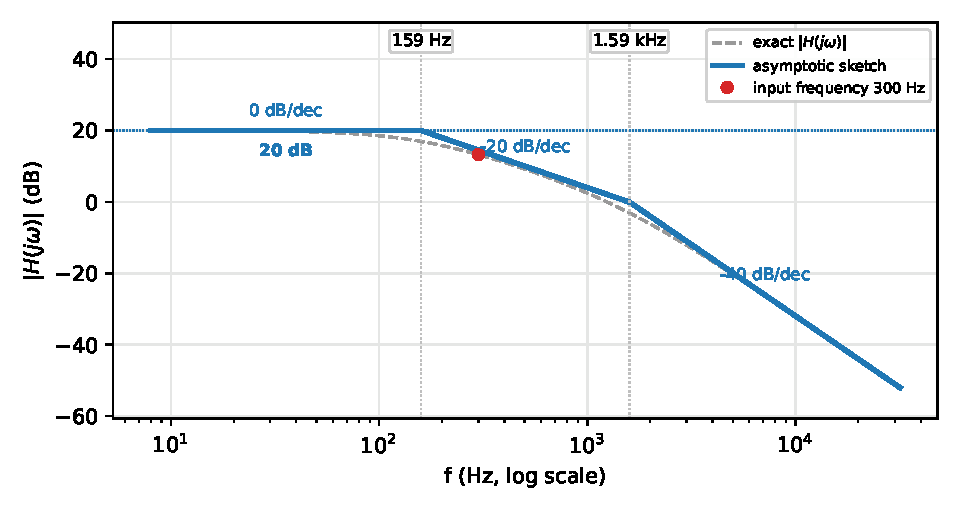
\includegraphics[width=0.78\linewidth,height=6.5cm,keepaspectratio]{p05_bode}\end{center}

{\small Blue: the straight-line sketch you are expected to draw. Dashed grey: the exact curve (about 3\,dB below the corner of an isolated pole). Red dot: the input frequency of Step 7.}
\solstep{7}{Steady-state output}The input is $V_i(t) = 0.05\sin\left(2\pi\cdot 300\,t\right)$, so $\omega_{in} = 2\pi\cdot 300 = 1880$\,rad/s. Put $s=j\omega_{in}$ in each factor (tool T5): magnitudes multiply, angles add.
{\small Rules: $\left|\frac{s}{s+p}\right| = \frac{\omega}{\sqrt{\omega^2+p^2}}$, $\angle = \frac{\pi}{2}-\tan^{-1}\frac{\omega}{p}$;\quad $\left|\frac{1}{1+s/p}\right| = \frac{1}{\sqrt{1+(\omega/p)^2}}$, $\angle = -\tan^{-1}\frac{\omega}{p}$;\quad $\left|1+\frac{s}{z}\right| = \sqrt{1+(\omega/z)^2}$, $\angle = \tan^{-1}\frac{\omega}{z}$;\quad a negative $K$ adds $-\pi$.}
\begin{center}\renewcommand{\arraystretch}{1.35}
\begin{tabular}{ccc}
\toprule
factor & magnitude & angle (rad) \\
\midrule
$10$ & $10$ & $0$ \\
$\rule[-1.7em]{0pt}{4em}\dfrac{1}{1+\dfrac{s}{2\pi\cdot 159}}$ & $0.4686$ & $-1.08$ \\
$\rule[-1.7em]{0pt}{4em}\dfrac{1}{1+\dfrac{s}{2\pi\cdot 1.59\mathrm{k}}}$ & $0.9827$ & $-0.186$ \\
\textbf{total} & $\mathbf{4.605}$ (product) & $\mathbf{-1.27}$ (sum) \\
\bottomrule
\end{tabular}\end{center}

\begin{align*}
|H(j\omega_{in})| &= 4.61, \qquad \angle H(j\omega_{in}) = -1.27\ \mathrm{rad} \\
v_{o,ac}(t) &= 4.61\times 0.05\,\sin\left(2\pi\cdot 300\,t - 1.27\right) = 0.23\,\sin\left(2\pi\cdot 300\,t - 1.27\right)
\end{align*}

\[
\boxed{V_o(t) = 0.23\,\sin\left(2\pi\cdot 300\,t - 1.27\right)\ \mathrm{V}}
\]

\begin{ansbox}
$H(s) = 10\,\dfrac{1}{1+\dfrac{s}{2\pi\cdot 159}}\,\dfrac{1}{1+\dfrac{s}{2\pi\cdot 1.59\mathrm{k}}}$\quad (corners: 159 Hz, 1.59 kHz)\\[4pt]
$V_o(t) = 0.23\,\sin\left(2\pi\cdot 300\,t - 1.27\right)\ \mathrm{V}$
\end{ansbox}

\newpage
\subsection*{Solution 1C.6 \hfill Easy}
\begin{center}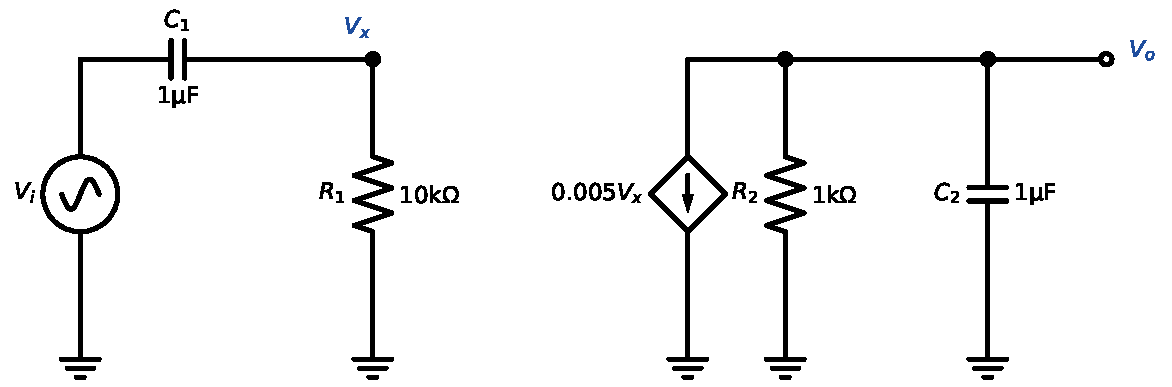
\includegraphics[width=0.8\linewidth,height=4.5cm,keepaspectratio]{p06_circuit}\end{center}
\solstep{1}{Identify the sources}Independent sources: the AC input $V_i(t)$. The diamond-shaped sources are \emph{dependent} sources: they are not inputs, they only copy/scale a voltage that already exists in the circuit, so they stay in the circuit in every step. There is no DC source, so $V_{o,dc}=0$ and $V_o(t)=v_{o,ac}(t)$: Step 2 is skipped.
\solstep{2}{DC circuit}No DC sources: $V_{o,dc}=0$.
\solstep{3}{AC circuit}Replace every capacitor by $\frac{1}{sC}$ and every inductor by $sL$.
AC equivalent circuit (nodes named for the next step):
\begin{center}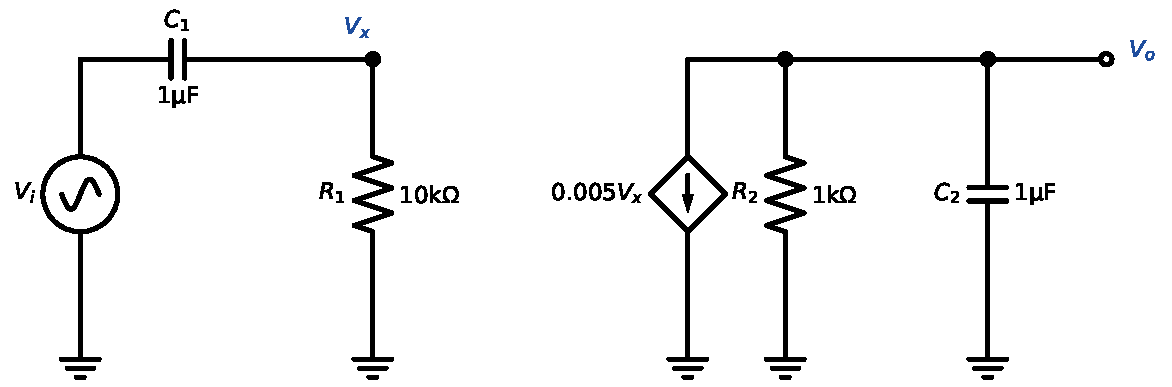
\includegraphics[width=0.95\linewidth,height=5.2cm,keepaspectratio]{p06_ac}\end{center}

\solstep{4}{Transfer function by a chain of dividers}Walk from the input to the output through the named nodes: $V_{i} \to V_{x} \to V_{o}$. The transfer function is the product of the node-to-node ratios (each one is a simple divider, tool T2, or a dependent source, tool T4):
\[
H(s) = \frac{V_o}{V_i} = \frac{V_{x}}{V_{i}}\cdot\frac{V_{o}}{V_{x}}
\]

Impedances seen \emph{looking right} from a node (everything from that node to ground, excluding what is on its left). Compute them from the far right toward the input:
\begin{align*}
Z_{o} &= R_{2} \parallel \frac{1}{sC_{2}} = \dfrac{10^{6}}{s + 1000}
\end{align*}

Now each link. {\small (Algebra tip: to simplify a fraction that contains fractions, multiply its top and bottom by every inner denominator; then divide top and bottom by the leading coefficient of the denominator so that it starts with a plain $s^n$.)}
\begin{align*}
\frac{V_{x}}{V_{i}} &= \frac{R_{1}}{\frac{1}{sC_{1}} + R_{1}} = \dfrac{s}{s + 100} \\
\frac{V_{o}}{V_{x}} &= -0.005\,Z_{o} = \dfrac{-5000}{s + 1000}
\end{align*}

(VCCS: the current $0.005V_{x}$ flows out of node $V_{o}$ and through $Z_{o}$ to ground, so $V_{o} = -0.005V_{x}\,Z_{o}$ by Ohm's law.)
Multiply the links and simplify (common factors cancel):\[
H(s) = \dfrac{-5000\,s}{s^{2} + 1100\,s + 10^{5}}
\]

\solstep{5}{Standard (Bode-ready) form}Find the roots. Every root $s=-p$ of the denominator is a \emph{pole}, every root $s=-z$ of the numerator is a \emph{zero}; $|p|$ and $|z|$ are the corner frequencies (rad/s).
\begin{itemize}[leftmargin=*,itemsep=2pt]
\item Numerator: it has the factor $s$ $\Rightarrow$ 1 zero at $s=0$.
\item Denominator: $s^{2} + 1100\,s + 10^{5}$; quadratic formula:\[
s = \frac{-1100 \pm \sqrt{(1100)^2 - 4(10^{5})}}{2} = \frac{-1100 \pm 900}{2} \Rightarrow s = -100,\ -1000
\]

\end{itemize}

Factored form (leading coefficient in front):
\[
H(s) = -5000\,\dfrac{s}{(s+100)(s+1000)}
\]

Bode-ready form: rewrite every $(s+p) = p\left(1+\frac{s}{p}\right)$ and $(s+z) = z\left(1+\frac{s}{z}\right)$, and collect all constants into $K$. Each $s$ in the numerator is paired with one of the \emph{lowest} poles as $\frac{s}{s+p}$ (that factor is $\approx 1$ above $p$). Then every factor except $K$ is $\approx 1$ inside the pass-band:
\[
H(s) = -5\,\dfrac{s}{s+2\pi\cdot 15.9}\,\dfrac{1}{1+\dfrac{s}{2\pi\cdot 159}},\qquad K = -5
\]

\begin{center}\renewcommand{\arraystretch}{1.35}
\begin{tabular}{cccc}
\toprule
type & $\omega_c$ (rad/s) & $f_c=\omega_c/2\pi$ & slope change \\
\midrule
pole & $100$ & 15.9 Hz & $-20$ dB/dec \\
pole & $1000$ & 159 Hz & $-20$ dB/dec \\
\bottomrule
\end{tabular}\end{center}

\solstep{6}{Magnitude Bode plot}Below every corner $|H(s)|\approx 0.05\,s$, so the plot starts with a slope of $+20$\,dB/dec. Then, moving right, each pole bends the line down by 20\,dB/dec and each zero bends it up by 20\,dB/dec (tool T6):
\begin{center}\renewcommand{\arraystretch}{1.35}
\begin{tabular}{lcl}
\toprule
frequency range & slope & asymptote level \\
\midrule
$f<$ 15.9 Hz & $+20$ dB/dec & 14 dB at end \\
15.9 Hz -- 159 Hz & $0$ dB/dec (flat) & 14 dB at start, 14 dB at end \\
$f>$ 159 Hz & $-20$ dB/dec & 14 dB at start \\
\bottomrule
\end{tabular}\end{center}

The flat (pass-band) level is $20\log_{10}|K| = 20\log_{10}5 = 14$\,dB.
\begin{center}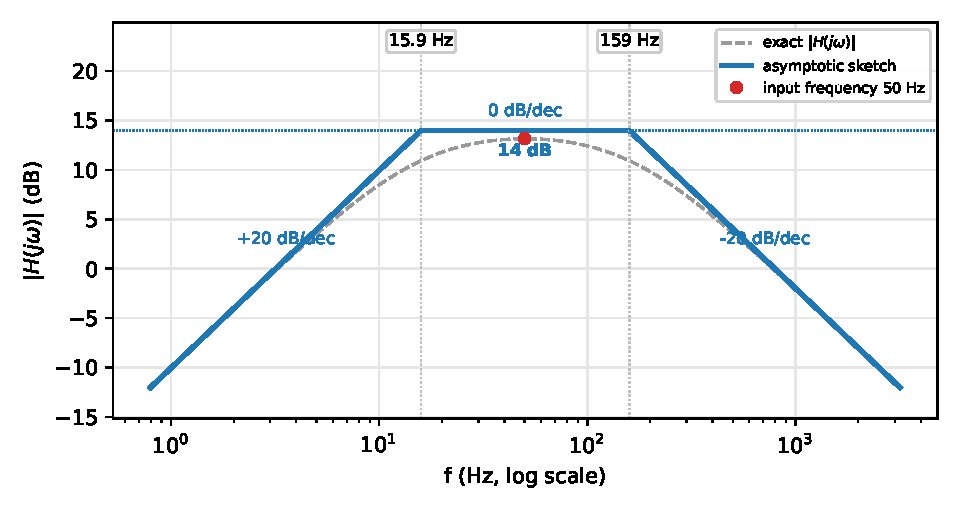
\includegraphics[width=0.78\linewidth,height=6.5cm,keepaspectratio]{p06_bode}\end{center}

{\small Blue: the straight-line sketch you are expected to draw. Dashed grey: the exact curve (about 3\,dB below the corner of an isolated pole). Red dot: the input frequency of Step 7.}
\solstep{7}{Steady-state output}The input is $V_i(t) = 0.2\sin\left(2\pi\cdot 50\,t\right)$, so $\omega_{in} = 2\pi\cdot 50 = 314$\,rad/s. Put $s=j\omega_{in}$ in each factor (tool T5): magnitudes multiply, angles add.
{\small Rules: $\left|\frac{s}{s+p}\right| = \frac{\omega}{\sqrt{\omega^2+p^2}}$, $\angle = \frac{\pi}{2}-\tan^{-1}\frac{\omega}{p}$;\quad $\left|\frac{1}{1+s/p}\right| = \frac{1}{\sqrt{1+(\omega/p)^2}}$, $\angle = -\tan^{-1}\frac{\omega}{p}$;\quad $\left|1+\frac{s}{z}\right| = \sqrt{1+(\omega/z)^2}$, $\angle = \tan^{-1}\frac{\omega}{z}$;\quad a negative $K$ adds $-\pi$.}
\begin{center}\renewcommand{\arraystretch}{1.35}
\begin{tabular}{ccc}
\toprule
factor & magnitude & angle (rad) \\
\midrule
$-5$ & $5$ & $-3.14$ \\
$\rule[-1.1em]{0pt}{2.8em}\dfrac{s}{s+2\pi\cdot 15.9}$ & $0.9529$ & $0.308$ \\
$\rule[-1.7em]{0pt}{4em}\dfrac{1}{1+\dfrac{s}{2\pi\cdot 159}}$ & $0.954$ & $-0.304$ \\
\textbf{total} & $\mathbf{4.545}$ (product) & $\mathbf{-3.14}$ (sum) \\
\bottomrule
\end{tabular}\end{center}

\begin{align*}
|H(j\omega_{in})| &= 4.55, \qquad \angle H(j\omega_{in}) = -3.14\ \mathrm{rad} \\
v_{o,ac}(t) &= 4.55\times 0.2\,\sin\left(2\pi\cdot 50\,t - 3.14\right) = 0.909\,\sin\left(2\pi\cdot 50\,t - 3.14\right)
\end{align*}

\[
\boxed{V_o(t) = 0.909\,\sin\left(2\pi\cdot 50\,t - 3.14\right)\ \mathrm{V}}
\]

\begin{ansbox}
$H(s) = -5\,\dfrac{s}{s+2\pi\cdot 15.9}\,\dfrac{1}{1+\dfrac{s}{2\pi\cdot 159}}$\quad (corners: 15.9 Hz, 159 Hz)\\[4pt]
$V_o(t) = 0.909\,\sin\left(2\pi\cdot 50\,t - 3.14\right)\ \mathrm{V}$
\end{ansbox}

\newpage
\subsection*{Solution 1C.7 \hfill Medium}
\begin{center}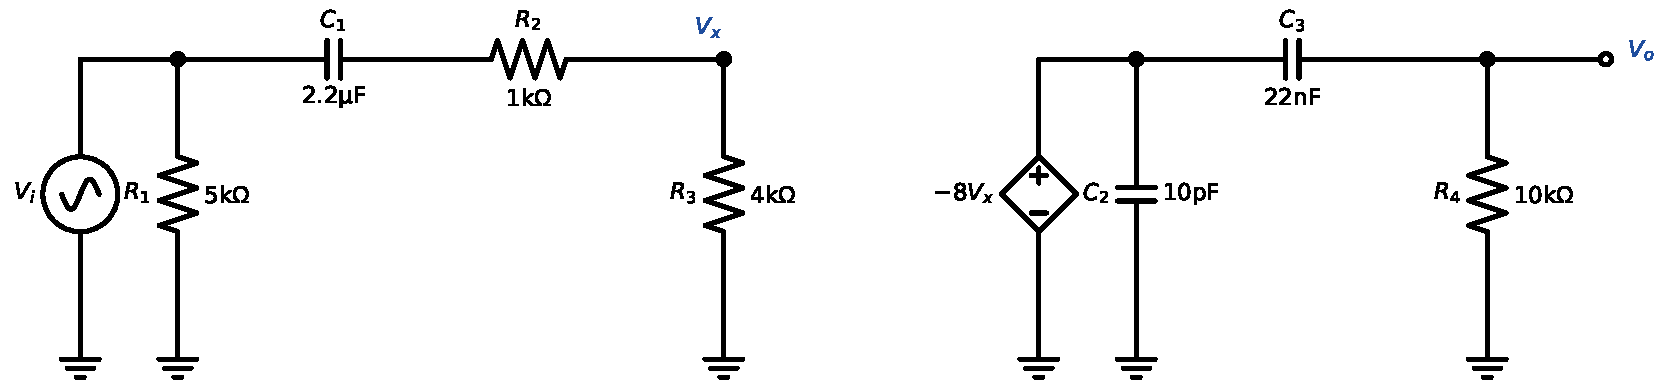
\includegraphics[width=0.8\linewidth,height=4.5cm,keepaspectratio]{p07_circuit}\end{center}
\solstep{1}{Identify the sources}Independent sources: the AC input $V_i(t)$. The diamond-shaped sources are \emph{dependent} sources: they are not inputs, they only copy/scale a voltage that already exists in the circuit, so they stay in the circuit in every step. There is no DC source, so $V_{o,dc}=0$ and $V_o(t)=v_{o,ac}(t)$: Step 2 is skipped.
\solstep{2}{DC circuit}No DC sources: $V_{o,dc}=0$.
\solstep{3}{AC circuit}Replace every capacitor by $\frac{1}{sC}$ and every inductor by $sL$.
\begin{itemize}[leftmargin=*,itemsep=2pt]
\item $R_{1}$ sits directly across the ideal input source $V_i$. An ideal voltage source keeps its voltage whatever you connect to it, so $R_{1}$ cannot change any node voltage: it drops out of $H(s)$.
\item $C_{2}$ sits directly across the output of the ideal dependent voltage source. An ideal voltage source keeps its voltage whatever you connect to it, so $C_{2}$ cannot change any node voltage: it drops out of $H(s)$.
\end{itemize}

AC equivalent circuit (nodes named for the next step):
\begin{center}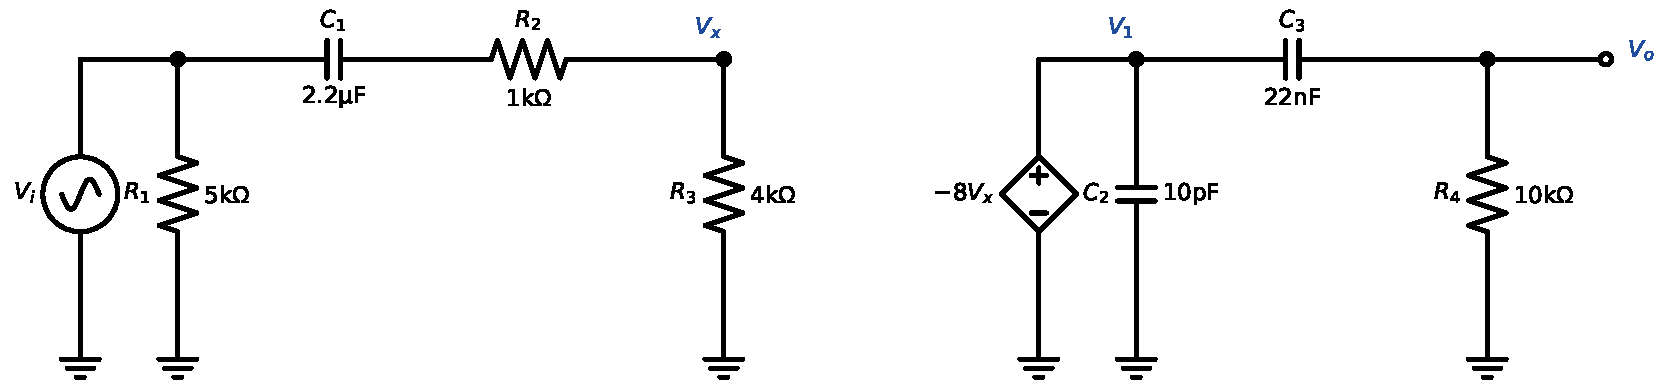
\includegraphics[width=0.95\linewidth,height=5.2cm,keepaspectratio]{p07_ac}\end{center}

\solstep{4}{Transfer function by a chain of dividers}Walk from the input to the output through the named nodes: $V_{i} \to V_{x} \to V_{1} \to V_{o}$. The transfer function is the product of the node-to-node ratios (each one is a simple divider, tool T2, or a dependent source, tool T4):
\[
H(s) = \frac{V_o}{V_i} = \frac{V_{x}}{V_{i}}\cdot\frac{V_{1}}{V_{x}}\cdot\frac{V_{o}}{V_{1}}
\]

Now each link. {\small (Algebra tip: to simplify a fraction that contains fractions, multiply its top and bottom by every inner denominator; then divide top and bottom by the leading coefficient of the denominator so that it starts with a plain $s^n$.)}
\begin{align*}
\frac{V_{x}}{V_{i}} &= \frac{R_{3}}{\frac{1}{sC_{1}} + R_{2} + R_{3}} = \dfrac{0.8\,s}{s + 90.9} \\
\frac{V_{1}}{V_{x}} &= -8 &&\text{(ideal VCVS: $V_{1} = -8V_{x}$)} \\
\frac{V_{o}}{V_{1}} &= \frac{R_{4}}{\frac{1}{sC_{3}} + R_{4}} = \dfrac{s}{s + 4550}
\end{align*}

Multiply the links and simplify (common factors cancel):\[
H(s) = \dfrac{-6.4\,s^{2}}{s^{2} + 4640\,s + 4.13\times 10^{5}}
\]

\solstep{5}{Standard (Bode-ready) form}Find the roots. Every root $s=-p$ of the denominator is a \emph{pole}, every root $s=-z$ of the numerator is a \emph{zero}; $|p|$ and $|z|$ are the corner frequencies (rad/s).
\begin{itemize}[leftmargin=*,itemsep=2pt]
\item Numerator: it has the factor $s^2$ $\Rightarrow$ 2 zeros at $s=0$.
\item Denominator: $s^{2} + 4640\,s + 4.13\times 10^{5}$; quadratic formula:\[
s = \frac{-4640 \pm \sqrt{(4640)^2 - 4(4.13\times 10^{5})}}{2} = \frac{-4640 \pm 4450}{2} \Rightarrow s = -90.9,\ -4550
\]

\end{itemize}

Factored form (leading coefficient in front):
\[
H(s) = -6.4\,\dfrac{s^{2}}{(s+90.9)(s+4550)}
\]

Bode-ready form: rewrite every $(s+p) = p\left(1+\frac{s}{p}\right)$ and $(s+z) = z\left(1+\frac{s}{z}\right)$, and collect all constants into $K$. Each $s$ in the numerator is paired with one of the \emph{lowest} poles as $\frac{s}{s+p}$ (that factor is $\approx 1$ above $p$). Then every factor except $K$ is $\approx 1$ inside the pass-band:
\[
H(s) = -6.4\,\dfrac{s}{s+2\pi\cdot 14.5}\,\dfrac{s}{s+2\pi\cdot 723},\qquad K = -6.4
\]

\begin{center}\renewcommand{\arraystretch}{1.35}
\begin{tabular}{cccc}
\toprule
type & $\omega_c$ (rad/s) & $f_c=\omega_c/2\pi$ & slope change \\
\midrule
pole & $90.9$ & 14.5 Hz & $-20$ dB/dec \\
pole & $4550$ & 723 Hz & $-20$ dB/dec \\
\bottomrule
\end{tabular}\end{center}

\solstep{6}{Magnitude Bode plot}Below every corner $|H(s)|\approx 1.55\times 10^{-5}\,s^2$, so the plot starts with a slope of $+40$\,dB/dec. Then, moving right, each pole bends the line down by 20\,dB/dec and each zero bends it up by 20\,dB/dec (tool T6):
\begin{center}\renewcommand{\arraystretch}{1.35}
\begin{tabular}{lcl}
\toprule
frequency range & slope & asymptote level \\
\midrule
$f<$ 14.5 Hz & $+40$ dB/dec & -17.9 dB at end \\
14.5 Hz -- 723 Hz & $+20$ dB/dec & -17.9 dB at start, 16.1 dB at end \\
$f>$ 723 Hz & $0$ dB/dec (flat) & 16.1 dB at start \\
\bottomrule
\end{tabular}\end{center}

The flat (pass-band) level is $20\log_{10}|K| = 20\log_{10}6.4 = 16.1$\,dB.
\begin{center}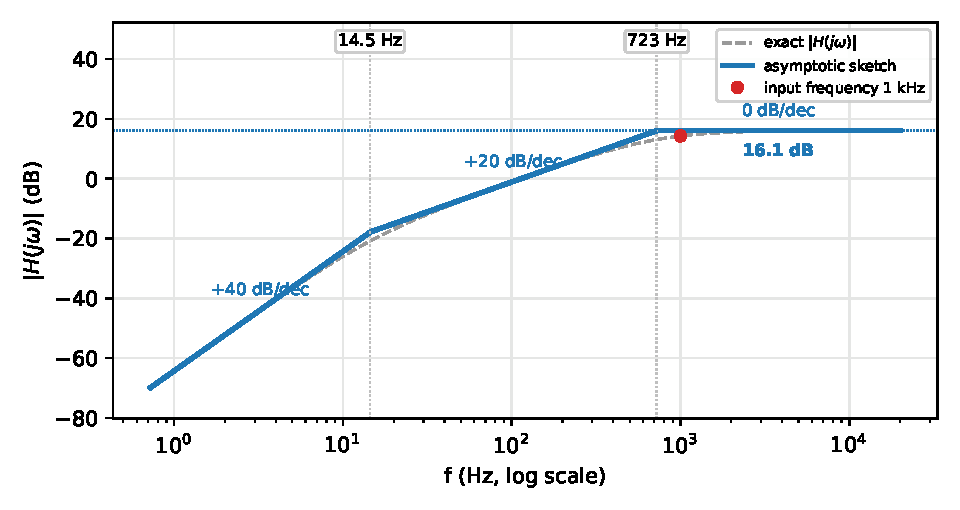
\includegraphics[width=0.78\linewidth,height=6.5cm,keepaspectratio]{p07_bode}\end{center}

{\small Blue: the straight-line sketch you are expected to draw. Dashed grey: the exact curve (about 3\,dB below the corner of an isolated pole). Red dot: the input frequency of Step 7.}
\solstep{7}{Steady-state output}The input is $V_i(t) = 0.1\sin\left(2\pi\cdot 1000\,t\right)$, so $\omega_{in} = 2\pi\cdot 1000 = 6280$\,rad/s. Put $s=j\omega_{in}$ in each factor (tool T5): magnitudes multiply, angles add.
{\small Rules: $\left|\frac{s}{s+p}\right| = \frac{\omega}{\sqrt{\omega^2+p^2}}$, $\angle = \frac{\pi}{2}-\tan^{-1}\frac{\omega}{p}$;\quad $\left|\frac{1}{1+s/p}\right| = \frac{1}{\sqrt{1+(\omega/p)^2}}$, $\angle = -\tan^{-1}\frac{\omega}{p}$;\quad $\left|1+\frac{s}{z}\right| = \sqrt{1+(\omega/z)^2}$, $\angle = \tan^{-1}\frac{\omega}{z}$;\quad a negative $K$ adds $-\pi$.}
\begin{center}\renewcommand{\arraystretch}{1.35}
\begin{tabular}{ccc}
\toprule
factor & magnitude & angle (rad) \\
\midrule
$-6.4$ & $6.4$ & $-3.14$ \\
$\rule[-1.1em]{0pt}{2.8em}\dfrac{s}{s+2\pi\cdot 14.5}$ & $0.9999$ & $0.0145$ \\
$\rule[-1.1em]{0pt}{2.8em}\dfrac{s}{s+2\pi\cdot 723}$ & $0.8102$ & $0.626$ \\
\textbf{total} & $\mathbf{5.185}$ (product) & $\mathbf{-2.5}$ (sum) \\
\bottomrule
\end{tabular}\end{center}

\begin{align*}
|H(j\omega_{in})| &= 5.18, \qquad \angle H(j\omega_{in}) = -2.5\ \mathrm{rad} \\
v_{o,ac}(t) &= 5.18\times 0.1\,\sin\left(2\pi\cdot 1000\,t - 2.5\right) = 0.518\,\sin\left(2\pi\cdot 1000\,t - 2.5\right)
\end{align*}

\[
\boxed{V_o(t) = 0.518\,\sin\left(2\pi\cdot 1000\,t - 2.5\right)\ \mathrm{V}}
\]

\begin{ansbox}
$H(s) = -6.4\,\dfrac{s}{s+2\pi\cdot 14.5}\,\dfrac{s}{s+2\pi\cdot 723}$\quad (corners: 14.5 Hz, 723 Hz)\\[4pt]
$V_o(t) = 0.518\,\sin\left(2\pi\cdot 1000\,t - 2.5\right)\ \mathrm{V}$
\end{ansbox}

\newpage
\subsection*{Solution 1C.8 \hfill Medium}
\begin{center}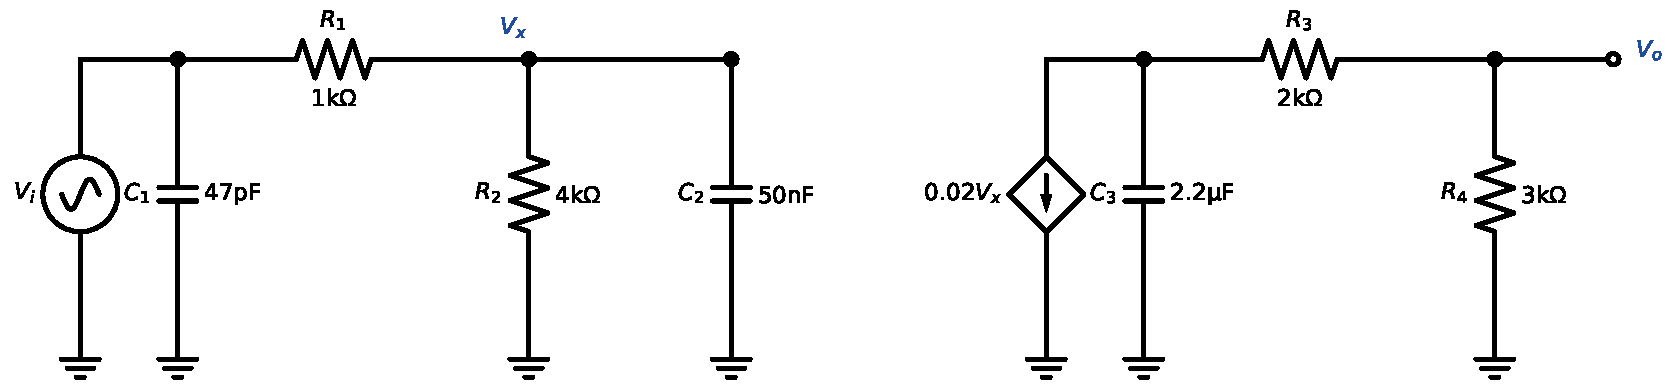
\includegraphics[width=0.8\linewidth,height=4.5cm,keepaspectratio]{p08_circuit}\end{center}
\solstep{1}{Identify the sources}Independent sources: the AC input $V_i(t)$. The diamond-shaped sources are \emph{dependent} sources: they are not inputs, they only copy/scale a voltage that already exists in the circuit, so they stay in the circuit in every step. There is no DC source, so $V_{o,dc}=0$ and $V_o(t)=v_{o,ac}(t)$: Step 2 is skipped.
\solstep{2}{DC circuit}No DC sources: $V_{o,dc}=0$.
\solstep{3}{AC circuit}Replace every capacitor by $\frac{1}{sC}$ and every inductor by $sL$.
\begin{itemize}[leftmargin=*,itemsep=2pt]
\item $C_{1}$ sits directly across the ideal input source $V_i$. An ideal voltage source keeps its voltage whatever you connect to it, so $C_{1}$ cannot change any node voltage: it drops out of $H(s)$.
\end{itemize}

AC equivalent circuit (nodes named for the next step):
\begin{center}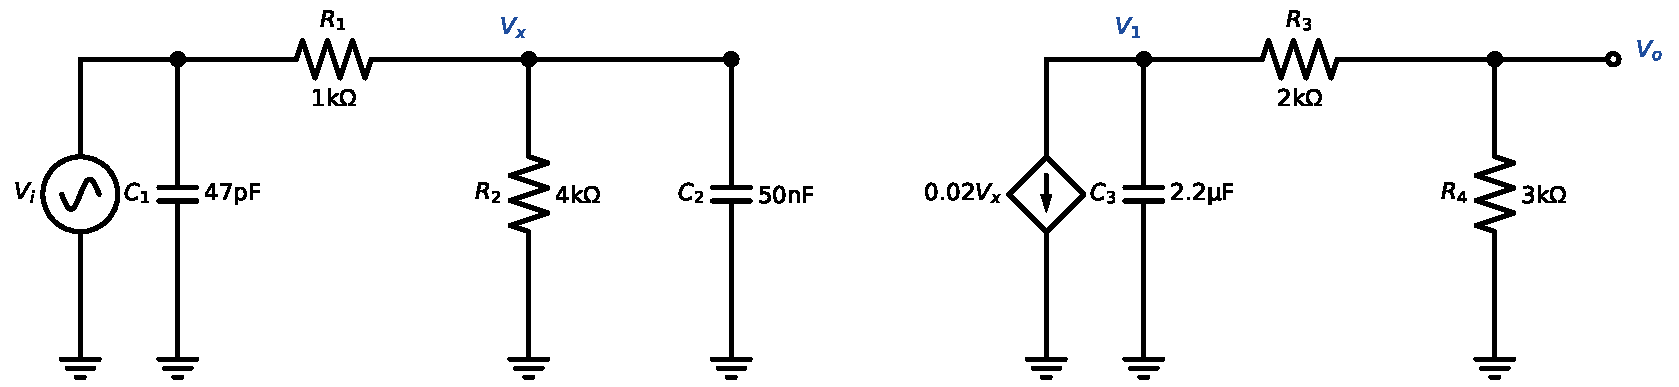
\includegraphics[width=0.95\linewidth,height=5.2cm,keepaspectratio]{p08_ac}\end{center}

\solstep{4}{Transfer function by a chain of dividers}Walk from the input to the output through the named nodes: $V_{i} \to V_{x} \to V_{1} \to V_{o}$. The transfer function is the product of the node-to-node ratios (each one is a simple divider, tool T2, or a dependent source, tool T4):
\[
H(s) = \frac{V_o}{V_i} = \frac{V_{x}}{V_{i}}\cdot\frac{V_{1}}{V_{x}}\cdot\frac{V_{o}}{V_{1}}
\]

Impedances seen \emph{looking right} from a node (everything from that node to ground, excluding what is on its left). Compute them from the far right toward the input:
\begin{align*}
Z_{x} &= R_{2} \parallel \frac{1}{sC_{2}} = \dfrac{2\times 10^{7}}{s + 5000} \\
Z_{1} &= \frac{1}{sC_{3}} \parallel \left(R_{3} + R_{4}\right) = \dfrac{4.55\times 10^{5}}{s + 90.9}
\end{align*}

Now each link. {\small (Algebra tip: to simplify a fraction that contains fractions, multiply its top and bottom by every inner denominator; then divide top and bottom by the leading coefficient of the denominator so that it starts with a plain $s^n$.)}
\begin{align*}
\frac{V_{x}}{V_{i}} &= \frac{Z_{x}}{R_{1} + Z_{x}} = \dfrac{20000}{s + 25000} \\
\frac{V_{1}}{V_{x}} &= -0.02\,Z_{1} = \dfrac{-9090}{s + 90.9} \\
\frac{V_{o}}{V_{1}} &= \frac{R_{4}}{R_{3} + R_{4}} = 0.6
\end{align*}

(VCCS: the current $0.02V_{x}$ flows out of node $V_{1}$ and through $Z_{1}$ to ground, so $V_{1} = -0.02V_{x}\,Z_{1}$ by Ohm's law.)
Multiply the links and simplify (common factors cancel):\[
H(s) = \dfrac{-1.09\times 10^{8}}{s^{2} + 25100\,s + 2.27\times 10^{6}}
\]

\solstep{5}{Standard (Bode-ready) form}Find the roots. Every root $s=-p$ of the denominator is a \emph{pole}, every root $s=-z$ of the numerator is a \emph{zero}; $|p|$ and $|z|$ are the corner frequencies (rad/s).
\begin{itemize}[leftmargin=*,itemsep=2pt]
\item Denominator: $s^{2} + 25100\,s + 2.27\times 10^{6}$; quadratic formula:\[
s = \frac{-25100 \pm \sqrt{(25100)^2 - 4(2.27\times 10^{6})}}{2} = \frac{-25100 \pm 24900}{2} \Rightarrow s = -90.9,\ -25000
\]

\end{itemize}

Factored form (leading coefficient in front):
\[
H(s) = -1.09\times 10^{8}\,\dfrac{1}{(s+90.9)(s+25000)}
\]

Bode-ready form: rewrite every $(s+p) = p\left(1+\frac{s}{p}\right)$ and $(s+z) = z\left(1+\frac{s}{z}\right)$, and collect all constants into $K$. Then every factor except $K$ is $\approx 1$ inside the pass-band:
\[
H(s) = -48\,\dfrac{1}{1+\dfrac{s}{2\pi\cdot 14.5}}\,\dfrac{1}{1+\dfrac{s}{2\pi\cdot 3.98\mathrm{k}}},\qquad K = -48
\]

\begin{center}\renewcommand{\arraystretch}{1.35}
\begin{tabular}{cccc}
\toprule
type & $\omega_c$ (rad/s) & $f_c=\omega_c/2\pi$ & slope change \\
\midrule
pole & $90.9$ & 14.5 Hz & $-20$ dB/dec \\
pole & $25000$ & 3.98 kHz & $-20$ dB/dec \\
\bottomrule
\end{tabular}\end{center}

\solstep{6}{Magnitude Bode plot}Below every corner, all factors are $\approx$ constant: $|H| \approx 48$ $= 33.6$\,dB (flat, 0 dB/dec). Then, moving right, each pole bends the line down by 20\,dB/dec and each zero bends it up by 20\,dB/dec (tool T6):
\begin{center}\renewcommand{\arraystretch}{1.35}
\begin{tabular}{lcl}
\toprule
frequency range & slope & asymptote level \\
\midrule
$f<$ 14.5 Hz & $0$ dB/dec (flat) & 33.6 dB at end \\
14.5 Hz -- 3.98 kHz & $-20$ dB/dec & 33.6 dB at start, -15.2 dB at end \\
$f>$ 3.98 kHz & $-40$ dB/dec & -15.2 dB at start \\
\bottomrule
\end{tabular}\end{center}

The flat (pass-band) level is $20\log_{10}|K| = 20\log_{10}48 = 33.6$\,dB.
\begin{center}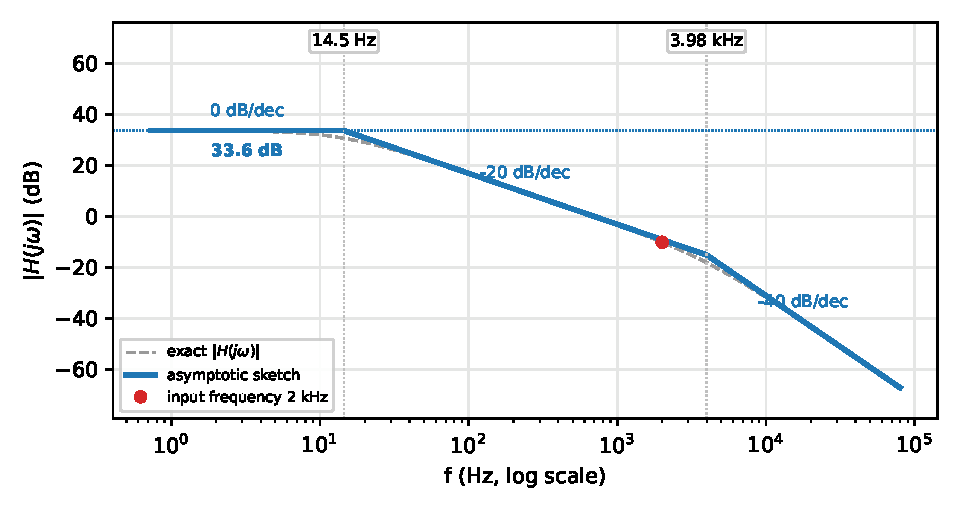
\includegraphics[width=0.78\linewidth,height=6.5cm,keepaspectratio]{p08_bode}\end{center}

{\small Blue: the straight-line sketch you are expected to draw. Dashed grey: the exact curve (about 3\,dB below the corner of an isolated pole). Red dot: the input frequency of Step 7.}
\solstep{7}{Steady-state output}The input is $V_i(t) = 0.05\sin\left(2\pi\cdot 2000\,t\right)$, so $\omega_{in} = 2\pi\cdot 2000 = 12600$\,rad/s. Put $s=j\omega_{in}$ in each factor (tool T5): magnitudes multiply, angles add.
{\small Rules: $\left|\frac{s}{s+p}\right| = \frac{\omega}{\sqrt{\omega^2+p^2}}$, $\angle = \frac{\pi}{2}-\tan^{-1}\frac{\omega}{p}$;\quad $\left|\frac{1}{1+s/p}\right| = \frac{1}{\sqrt{1+(\omega/p)^2}}$, $\angle = -\tan^{-1}\frac{\omega}{p}$;\quad $\left|1+\frac{s}{z}\right| = \sqrt{1+(\omega/z)^2}$, $\angle = \tan^{-1}\frac{\omega}{z}$;\quad a negative $K$ adds $-\pi$.}
\begin{center}\renewcommand{\arraystretch}{1.35}
\begin{tabular}{ccc}
\toprule
factor & magnitude & angle (rad) \\
\midrule
$-48$ & $48$ & $-3.14$ \\
$\rule[-1.7em]{0pt}{4em}\dfrac{1}{1+\dfrac{s}{2\pi\cdot 14.5}}$ & $0.007234$ & $-1.56$ \\
$\rule[-1.7em]{0pt}{4em}\dfrac{1}{1+\dfrac{s}{2\pi\cdot 3.98\mathrm{k}}}$ & $0.8935$ & $-0.466$ \\
\textbf{total} & $\mathbf{0.3102}$ (product) & $\mathbf{-5.17}$ (sum) \\
\bottomrule
\end{tabular}\end{center}

\begin{align*}
|H(j\omega_{in})| &= 0.31, \qquad \angle H(j\omega_{in}) = -5.17\ \mathrm{rad} \\
v_{o,ac}(t) &= 0.31\times 0.05\,\sin\left(2\pi\cdot 2000\,t - 5.17\right) = 0.0155\,\sin\left(2\pi\cdot 2000\,t - 5.17\right)
\end{align*}

\[
\boxed{V_o(t) = 0.0155\,\sin\left(2\pi\cdot 2000\,t - 5.17\right)\ \mathrm{V}}
\]

\begin{ansbox}
$H(s) = -48\,\dfrac{1}{1+\dfrac{s}{2\pi\cdot 14.5}}\,\dfrac{1}{1+\dfrac{s}{2\pi\cdot 3.98\mathrm{k}}}$\quad (corners: 14.5 Hz, 3.98 kHz)\\[4pt]
$V_o(t) = 0.0155\,\sin\left(2\pi\cdot 2000\,t - 5.17\right)\ \mathrm{V}$
\end{ansbox}

\newpage
\subsection*{Solution 1C.9 \hfill Medium}
\begin{center}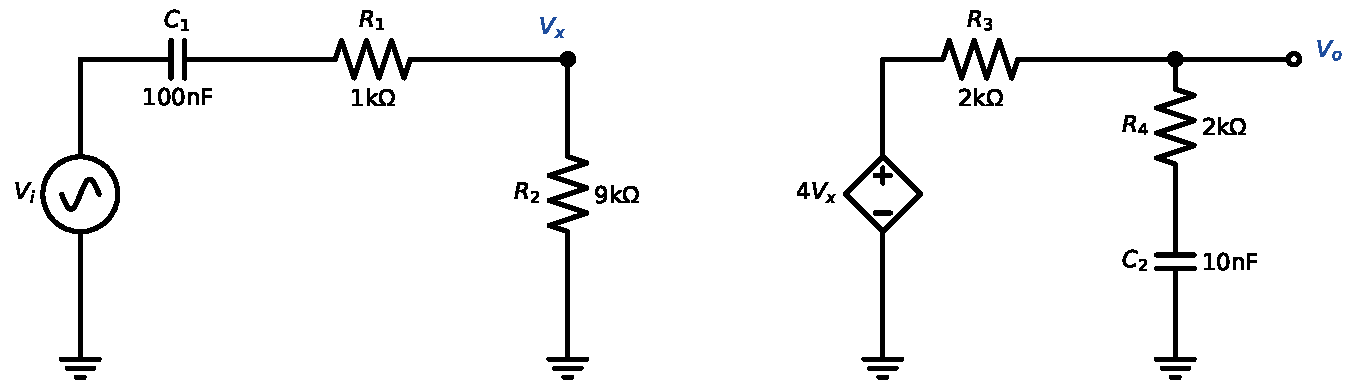
\includegraphics[width=0.8\linewidth,height=4.5cm,keepaspectratio]{p09_circuit}\end{center}
\solstep{1}{Identify the sources}Independent sources: the AC input $V_i(t)$. The diamond-shaped sources are \emph{dependent} sources: they are not inputs, they only copy/scale a voltage that already exists in the circuit, so they stay in the circuit in every step. There is no DC source, so $V_{o,dc}=0$ and $V_o(t)=v_{o,ac}(t)$: Step 2 is skipped.
\solstep{2}{DC circuit}No DC sources: $V_{o,dc}=0$.
\solstep{3}{AC circuit}Replace every capacitor by $\frac{1}{sC}$ and every inductor by $sL$.
AC equivalent circuit (nodes named for the next step):
\begin{center}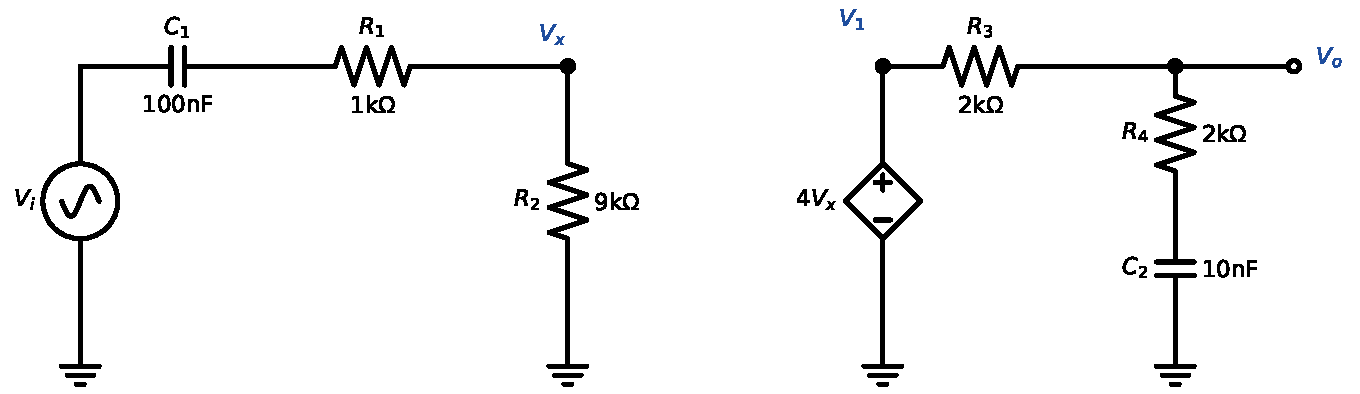
\includegraphics[width=0.95\linewidth,height=5.2cm,keepaspectratio]{p09_ac}\end{center}

\solstep{4}{Transfer function by a chain of dividers}Walk from the input to the output through the named nodes: $V_{i} \to V_{x} \to V_{1} \to V_{o}$. The transfer function is the product of the node-to-node ratios (each one is a simple divider, tool T2, or a dependent source, tool T4):
\[
H(s) = \frac{V_o}{V_i} = \frac{V_{x}}{V_{i}}\cdot\frac{V_{1}}{V_{x}}\cdot\frac{V_{o}}{V_{1}}
\]

Impedances seen \emph{looking right} from a node (everything from that node to ground, excluding what is on its left). Compute them from the far right toward the input:
\begin{align*}
Z_{o} &= R_{4} + \frac{1}{sC_{2}} = \dfrac{2000\,s + 10^{8}}{s}
\end{align*}

Now each link. {\small (Algebra tip: to simplify a fraction that contains fractions, multiply its top and bottom by every inner denominator; then divide top and bottom by the leading coefficient of the denominator so that it starts with a plain $s^n$.)}
\begin{align*}
\frac{V_{x}}{V_{i}} &= \frac{R_{2}}{\frac{1}{sC_{1}} + R_{1} + R_{2}} = \dfrac{0.9\,s}{s + 1000} \\
\frac{V_{1}}{V_{x}} &= 4 &&\text{(ideal VCVS: $V_{1} = 4V_{x}$)} \\
\frac{V_{o}}{V_{1}} &= \frac{Z_{o}}{R_{3} + Z_{o}} = \dfrac{0.5\,s + 25000}{s + 25000}
\end{align*}

Multiply the links and simplify (common factors cancel):\[
H(s) = \dfrac{1.8\,s^{2} + 90000\,s}{s^{2} + 26000\,s + 2.5\times 10^{7}}
\]

\solstep{5}{Standard (Bode-ready) form}Find the roots. Every root $s=-p$ of the denominator is a \emph{pole}, every root $s=-z$ of the numerator is a \emph{zero}; $|p|$ and $|z|$ are the corner frequencies (rad/s).
\begin{itemize}[leftmargin=*,itemsep=2pt]
\item Numerator: it has the factor $s$ $\Rightarrow$ 1 zero at $s=0$.
\item Numerator (after taking out the $s$ factor): $1.8\,s + 90000$; divide by the leading coefficient $1.8$ (this does not move the roots): $s + 50000$; $s + 50000 = 0 \Rightarrow s = -50000$.
\item Denominator: $s^{2} + 26000\,s + 2.5\times 10^{7}$; quadratic formula:\[
s = \frac{-26000 \pm \sqrt{(26000)^2 - 4(2.5\times 10^{7})}}{2} = \frac{-26000 \pm 24000}{2} \Rightarrow s = -1000,\ -25000
\]

\end{itemize}

Factored form (leading coefficient in front):
\[
H(s) = 1.8\,\dfrac{s(s+50000)}{(s+1000)(s+25000)}
\]

Bode-ready form: rewrite every $(s+p) = p\left(1+\frac{s}{p}\right)$ and $(s+z) = z\left(1+\frac{s}{z}\right)$, and collect all constants into $K$. Each $s$ in the numerator is paired with one of the \emph{lowest} poles as $\frac{s}{s+p}$ (that factor is $\approx 1$ above $p$). Then every factor except $K$ is $\approx 1$ inside the pass-band:
\[
H(s) = 3.6\,\dfrac{s}{s+2\pi\cdot 159}\,\dfrac{1}{1+\dfrac{s}{2\pi\cdot 3.98\mathrm{k}}}\,\left(1+\dfrac{s}{2\pi\cdot 7.96\mathrm{k}}\right),\qquad K = 3.6
\]

\begin{center}\renewcommand{\arraystretch}{1.35}
\begin{tabular}{cccc}
\toprule
type & $\omega_c$ (rad/s) & $f_c=\omega_c/2\pi$ & slope change \\
\midrule
pole & $1000$ & 159 Hz & $-20$ dB/dec \\
pole & $25000$ & 3.98 kHz & $-20$ dB/dec \\
zero & $50000$ & 7.96 kHz & $+20$ dB/dec \\
\bottomrule
\end{tabular}\end{center}

\solstep{6}{Magnitude Bode plot}Below every corner $|H(s)|\approx 0.0036\,s$, so the plot starts with a slope of $+20$\,dB/dec. Then, moving right, each pole bends the line down by 20\,dB/dec and each zero bends it up by 20\,dB/dec (tool T6):
\begin{center}\renewcommand{\arraystretch}{1.35}
\begin{tabular}{lcl}
\toprule
frequency range & slope & asymptote level \\
\midrule
$f<$ 159 Hz & $+20$ dB/dec & 11.1 dB at end \\
159 Hz -- 3.98 kHz & $0$ dB/dec (flat) & 11.1 dB at start, 11.1 dB at end \\
3.98 kHz -- 7.96 kHz & $-20$ dB/dec & 11.1 dB at start, 5.11 dB at end \\
$f>$ 7.96 kHz & $0$ dB/dec (flat) & 5.11 dB at start \\
\bottomrule
\end{tabular}\end{center}

\begin{center}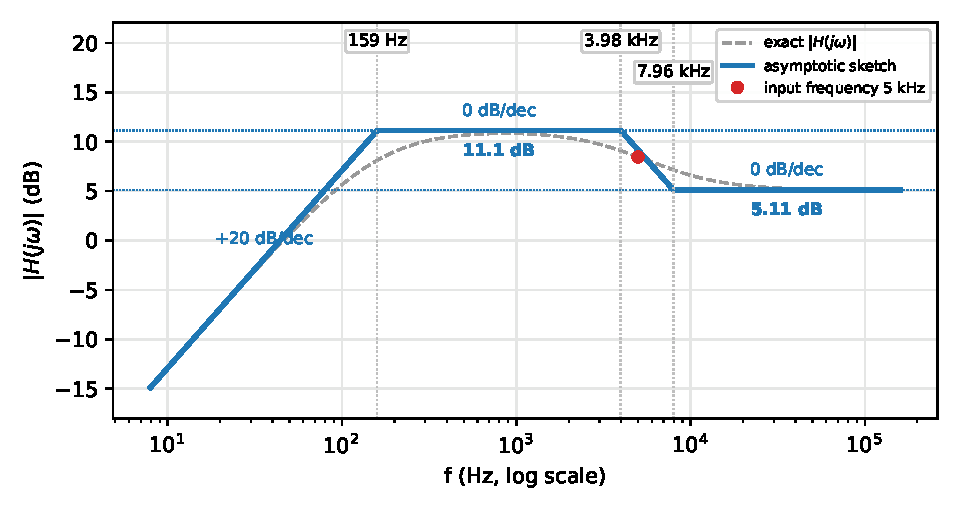
\includegraphics[width=0.78\linewidth,height=6.5cm,keepaspectratio]{p09_bode}\end{center}

{\small Blue: the straight-line sketch you are expected to draw. Dashed grey: the exact curve (about 3\,dB below the corner of an isolated pole). Red dot: the input frequency of Step 7.}
\solstep{7}{Steady-state output}The input is $V_i(t) = 0.2\sin\left(2\pi\cdot 5000\,t\right)$, so $\omega_{in} = 2\pi\cdot 5000 = 31400$\,rad/s. Put $s=j\omega_{in}$ in each factor (tool T5): magnitudes multiply, angles add.
{\small Rules: $\left|\frac{s}{s+p}\right| = \frac{\omega}{\sqrt{\omega^2+p^2}}$, $\angle = \frac{\pi}{2}-\tan^{-1}\frac{\omega}{p}$;\quad $\left|\frac{1}{1+s/p}\right| = \frac{1}{\sqrt{1+(\omega/p)^2}}$, $\angle = -\tan^{-1}\frac{\omega}{p}$;\quad $\left|1+\frac{s}{z}\right| = \sqrt{1+(\omega/z)^2}$, $\angle = \tan^{-1}\frac{\omega}{z}$;\quad a negative $K$ adds $-\pi$.}
\begin{center}\renewcommand{\arraystretch}{1.35}
\begin{tabular}{ccc}
\toprule
factor & magnitude & angle (rad) \\
\midrule
$3.6$ & $3.6$ & $0$ \\
$\rule[-1.1em]{0pt}{2.8em}\dfrac{s}{s+2\pi\cdot 159}$ & $0.9995$ & $0.0318$ \\
$\rule[-1.7em]{0pt}{4em}\dfrac{1}{1+\dfrac{s}{2\pi\cdot 3.98\mathrm{k}}}$ & $0.6227$ & $-0.899$ \\
$\rule[-1.1em]{0pt}{2.8em}\left(1+\dfrac{s}{2\pi\cdot 7.96\mathrm{k}}\right)$ & $1.181$ & $0.561$ \\
\textbf{total} & $\mathbf{2.646}$ (product) & $\mathbf{-0.306}$ (sum) \\
\bottomrule
\end{tabular}\end{center}

\begin{align*}
|H(j\omega_{in})| &= 2.65, \qquad \angle H(j\omega_{in}) = -0.306\ \mathrm{rad} \\
v_{o,ac}(t) &= 2.65\times 0.2\,\sin\left(2\pi\cdot 5000\,t - 0.306\right) = 0.529\,\sin\left(2\pi\cdot 5000\,t - 0.306\right)
\end{align*}

\[
\boxed{V_o(t) = 0.529\,\sin\left(2\pi\cdot 5000\,t - 0.306\right)\ \mathrm{V}}
\]

\begin{ansbox}
$H(s) = 3.6\,\dfrac{s}{s+2\pi\cdot 159}\,\dfrac{1}{1+\dfrac{s}{2\pi\cdot 3.98\mathrm{k}}}\,\left(1+\dfrac{s}{2\pi\cdot 7.96\mathrm{k}}\right)$\quad (corners: 159 Hz, 3.98 kHz, 7.96 kHz)\\[4pt]
$V_o(t) = 0.529\,\sin\left(2\pi\cdot 5000\,t - 0.306\right)\ \mathrm{V}$
\end{ansbox}

\newpage
\subsection*{Solution 1C.10 \hfill Medium}
\begin{center}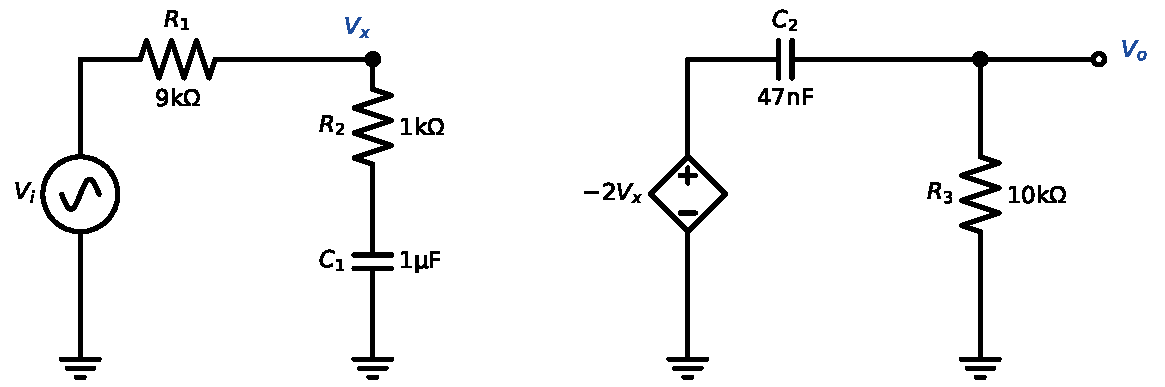
\includegraphics[width=0.8\linewidth,height=4.5cm,keepaspectratio]{p10_circuit}\end{center}
\solstep{1}{Identify the sources}Independent sources: the AC input $V_i(t)$. The diamond-shaped sources are \emph{dependent} sources: they are not inputs, they only copy/scale a voltage that already exists in the circuit, so they stay in the circuit in every step. There is no DC source, so $V_{o,dc}=0$ and $V_o(t)=v_{o,ac}(t)$: Step 2 is skipped.
\solstep{2}{DC circuit}No DC sources: $V_{o,dc}=0$.
\solstep{3}{AC circuit}Replace every capacitor by $\frac{1}{sC}$ and every inductor by $sL$.
AC equivalent circuit (nodes named for the next step):
\begin{center}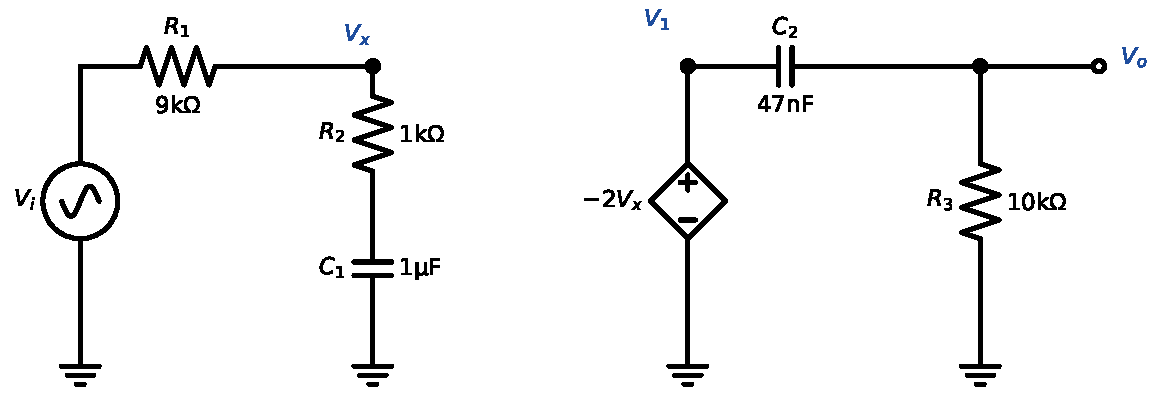
\includegraphics[width=0.95\linewidth,height=5.2cm,keepaspectratio]{p10_ac}\end{center}

\solstep{4}{Transfer function by a chain of dividers}Walk from the input to the output through the named nodes: $V_{i} \to V_{x} \to V_{1} \to V_{o}$. The transfer function is the product of the node-to-node ratios (each one is a simple divider, tool T2, or a dependent source, tool T4):
\[
H(s) = \frac{V_o}{V_i} = \frac{V_{x}}{V_{i}}\cdot\frac{V_{1}}{V_{x}}\cdot\frac{V_{o}}{V_{1}}
\]

Impedances seen \emph{looking right} from a node (everything from that node to ground, excluding what is on its left). Compute them from the far right toward the input:
\begin{align*}
Z_{x} &= R_{2} + \frac{1}{sC_{1}} = \dfrac{1000\,s + 10^{6}}{s}
\end{align*}

Now each link. {\small (Algebra tip: to simplify a fraction that contains fractions, multiply its top and bottom by every inner denominator; then divide top and bottom by the leading coefficient of the denominator so that it starts with a plain $s^n$.)}
\begin{align*}
\frac{V_{x}}{V_{i}} &= \frac{Z_{x}}{R_{1} + Z_{x}} = \dfrac{0.1\,s + 100}{s + 100} \\
\frac{V_{1}}{V_{x}} &= -2 &&\text{(ideal VCVS: $V_{1} = -2V_{x}$)} \\
\frac{V_{o}}{V_{1}} &= \frac{R_{3}}{\frac{1}{sC_{2}} + R_{3}} = \dfrac{s}{s + 2130}
\end{align*}

Multiply the links and simplify (common factors cancel):\[
H(s) = \dfrac{-0.2\,s^{2} - 200\,s}{s^{2} + 2230\,s + 2.13\times 10^{5}}
\]

\solstep{5}{Standard (Bode-ready) form}Find the roots. Every root $s=-p$ of the denominator is a \emph{pole}, every root $s=-z$ of the numerator is a \emph{zero}; $|p|$ and $|z|$ are the corner frequencies (rad/s).
\begin{itemize}[leftmargin=*,itemsep=2pt]
\item Numerator: it has the factor $s$ $\Rightarrow$ 1 zero at $s=0$.
\item Numerator (after taking out the $s$ factor): $-0.2\,s - 200$; divide by the leading coefficient $-0.2$ (this does not move the roots): $s + 1000$; $s + 1000 = 0 \Rightarrow s = -1000$.
\item Denominator: $s^{2} + 2230\,s + 2.13\times 10^{5}$; quadratic formula:\[
s = \frac{-2230 \pm \sqrt{(2230)^2 - 4(2.13\times 10^{5})}}{2} = \frac{-2230 \pm 2030}{2} \Rightarrow s = -100,\ -2130
\]

\end{itemize}

Factored form (leading coefficient in front):
\[
H(s) = -0.2\,\dfrac{s(s+1000)}{(s+100)(s+2130)}
\]

Bode-ready form: rewrite every $(s+p) = p\left(1+\frac{s}{p}\right)$ and $(s+z) = z\left(1+\frac{s}{z}\right)$, and collect all constants into $K$. Each $s$ in the numerator is paired with one of the \emph{lowest} poles as $\frac{s}{s+p}$ (that factor is $\approx 1$ above $p$). Then every factor except $K$ is $\approx 1$ inside the pass-band:
\[
H(s) = -0.094\,\dfrac{s}{s+2\pi\cdot 15.9}\,\left(1+\dfrac{s}{2\pi\cdot 159}\right)\,\dfrac{1}{1+\dfrac{s}{2\pi\cdot 339}},\qquad K = -0.094
\]

\begin{center}\renewcommand{\arraystretch}{1.35}
\begin{tabular}{cccc}
\toprule
type & $\omega_c$ (rad/s) & $f_c=\omega_c/2\pi$ & slope change \\
\midrule
pole & $100$ & 15.9 Hz & $-20$ dB/dec \\
zero & $1000$ & 159 Hz & $+20$ dB/dec \\
pole & $2130$ & 339 Hz & $-20$ dB/dec \\
\bottomrule
\end{tabular}\end{center}

\solstep{6}{Magnitude Bode plot}Below every corner $|H(s)|\approx 9.4\times 10^{-4}\,s$, so the plot starts with a slope of $+20$\,dB/dec. Then, moving right, each pole bends the line down by 20\,dB/dec and each zero bends it up by 20\,dB/dec (tool T6):
\begin{center}\renewcommand{\arraystretch}{1.35}
\begin{tabular}{lcl}
\toprule
frequency range & slope & asymptote level \\
\midrule
$f<$ 15.9 Hz & $+20$ dB/dec & -20.5 dB at end \\
15.9 Hz -- 159 Hz & $0$ dB/dec (flat) & -20.5 dB at start, -20.5 dB at end \\
159 Hz -- 339 Hz & $+20$ dB/dec & -20.5 dB at start, -14 dB at end \\
$f>$ 339 Hz & $0$ dB/dec (flat) & -14 dB at start \\
\bottomrule
\end{tabular}\end{center}

\begin{center}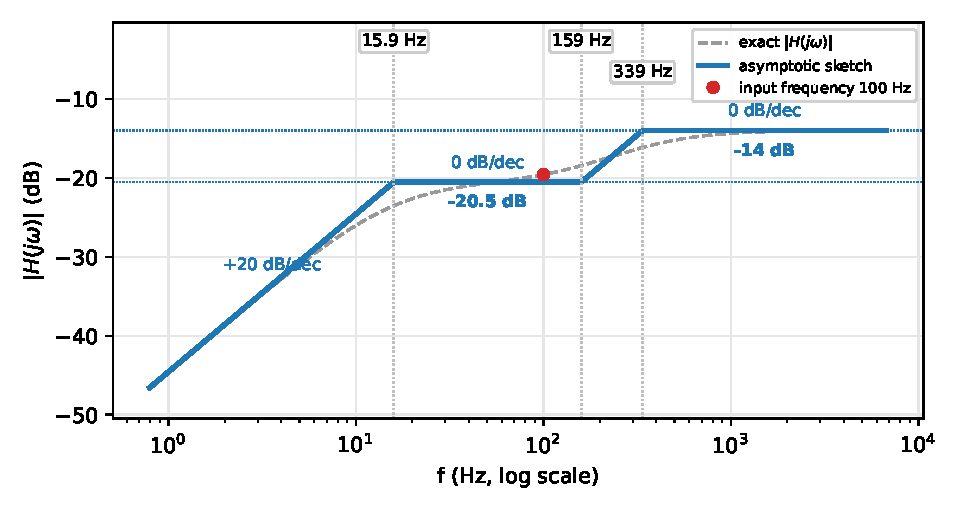
\includegraphics[width=0.78\linewidth,height=6.5cm,keepaspectratio]{p10_bode}\end{center}

{\small Blue: the straight-line sketch you are expected to draw. Dashed grey: the exact curve (about 3\,dB below the corner of an isolated pole). Red dot: the input frequency of Step 7.}
\solstep{7}{Steady-state output}The input is $V_i(t) = 0.5\sin\left(2\pi\cdot 100\,t\right)$, so $\omega_{in} = 2\pi\cdot 100 = 628$\,rad/s. Put $s=j\omega_{in}$ in each factor (tool T5): magnitudes multiply, angles add.
{\small Rules: $\left|\frac{s}{s+p}\right| = \frac{\omega}{\sqrt{\omega^2+p^2}}$, $\angle = \frac{\pi}{2}-\tan^{-1}\frac{\omega}{p}$;\quad $\left|\frac{1}{1+s/p}\right| = \frac{1}{\sqrt{1+(\omega/p)^2}}$, $\angle = -\tan^{-1}\frac{\omega}{p}$;\quad $\left|1+\frac{s}{z}\right| = \sqrt{1+(\omega/z)^2}$, $\angle = \tan^{-1}\frac{\omega}{z}$;\quad a negative $K$ adds $-\pi$.}
\begin{center}\renewcommand{\arraystretch}{1.35}
\begin{tabular}{ccc}
\toprule
factor & magnitude & angle (rad) \\
\midrule
$-0.094$ & $0.094$ & $-3.14$ \\
$\rule[-1.1em]{0pt}{2.8em}\dfrac{s}{s+2\pi\cdot 15.9}$ & $0.9876$ & $0.158$ \\
$\rule[-1.1em]{0pt}{2.8em}\left(1+\dfrac{s}{2\pi\cdot 159}\right)$ & $1.181$ & $0.561$ \\
$\rule[-1.7em]{0pt}{4em}\dfrac{1}{1+\dfrac{s}{2\pi\cdot 339}}$ & $0.9591$ & $-0.287$ \\
\textbf{total} & $\mathbf{0.1051}$ (product) & $\mathbf{-2.71}$ (sum) \\
\bottomrule
\end{tabular}\end{center}

\begin{align*}
|H(j\omega_{in})| &= 0.105, \qquad \angle H(j\omega_{in}) = -2.71\ \mathrm{rad} \\
v_{o,ac}(t) &= 0.105\times 0.5\,\sin\left(2\pi\cdot 100\,t - 2.71\right) = 0.0526\,\sin\left(2\pi\cdot 100\,t - 2.71\right)
\end{align*}

\[
\boxed{V_o(t) = 0.0526\,\sin\left(2\pi\cdot 100\,t - 2.71\right)\ \mathrm{V}}
\]

\begin{ansbox}
$H(s) = -0.094\,\dfrac{s}{s+2\pi\cdot 15.9}\,\left(1+\dfrac{s}{2\pi\cdot 159}\right)\,\dfrac{1}{1+\dfrac{s}{2\pi\cdot 339}}$\quad (corners: 15.9 Hz, 159 Hz, 339 Hz)\\[4pt]
$V_o(t) = 0.0526\,\sin\left(2\pi\cdot 100\,t - 2.71\right)\ \mathrm{V}$
\end{ansbox}

\newpage
\subsection*{Solution 1C.11 \hfill Medium}
\begin{center}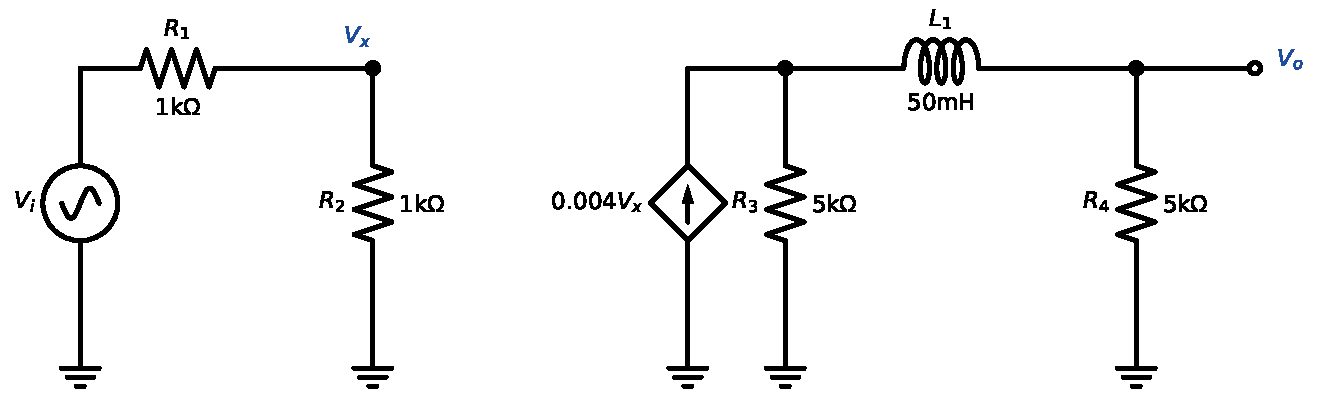
\includegraphics[width=0.8\linewidth,height=4.5cm,keepaspectratio]{p11_circuit}\end{center}
\solstep{1}{Identify the sources}Independent sources: the AC input $V_i(t)$. The diamond-shaped sources are \emph{dependent} sources: they are not inputs, they only copy/scale a voltage that already exists in the circuit, so they stay in the circuit in every step. There is no DC source, so $V_{o,dc}=0$ and $V_o(t)=v_{o,ac}(t)$: Step 2 is skipped.
\solstep{2}{DC circuit}No DC sources: $V_{o,dc}=0$.
\solstep{3}{AC circuit}Replace every capacitor by $\frac{1}{sC}$ and every inductor by $sL$.
AC equivalent circuit (nodes named for the next step):
\begin{center}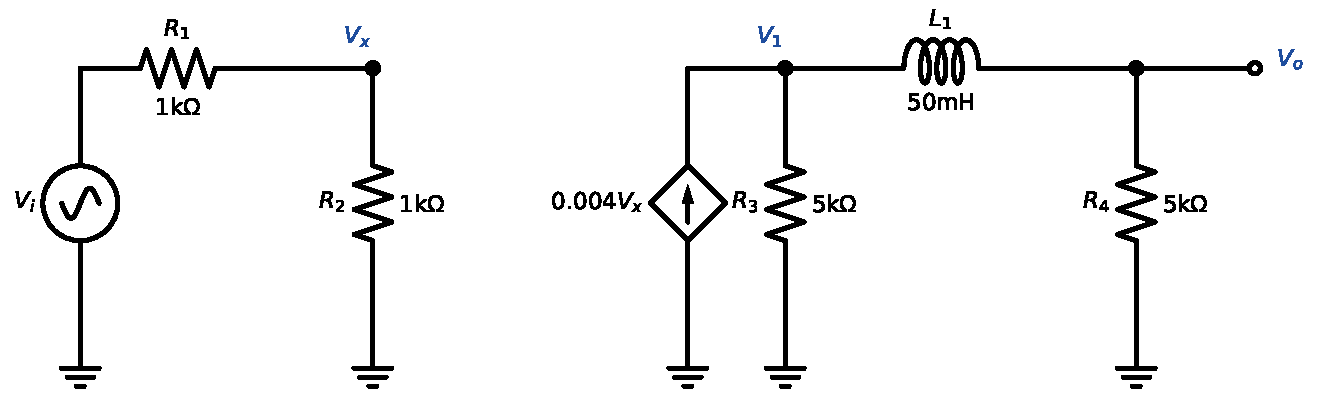
\includegraphics[width=0.95\linewidth,height=5.2cm,keepaspectratio]{p11_ac}\end{center}

\solstep{4}{Transfer function by a chain of dividers}Walk from the input to the output through the named nodes: $V_{i} \to V_{x} \to V_{1} \to V_{o}$. The transfer function is the product of the node-to-node ratios (each one is a simple divider, tool T2, or a dependent source, tool T4):
\[
H(s) = \frac{V_o}{V_i} = \frac{V_{x}}{V_{i}}\cdot\frac{V_{1}}{V_{x}}\cdot\frac{V_{o}}{V_{1}}
\]

Impedances seen \emph{looking right} from a node (everything from that node to ground, excluding what is on its left). Compute them from the far right toward the input:
\begin{align*}
Z_{1} &= R_{3} \parallel \left(sL_{1} + R_{4}\right) = \dfrac{5000\,s + 5\times 10^{8}}{s + 2\times 10^{5}}
\end{align*}

Now each link. {\small (Algebra tip: to simplify a fraction that contains fractions, multiply its top and bottom by every inner denominator; then divide top and bottom by the leading coefficient of the denominator so that it starts with a plain $s^n$.)}
\begin{align*}
\frac{V_{x}}{V_{i}} &= \frac{R_{2}}{R_{1} + R_{2}} = 0.5 \\
\frac{V_{1}}{V_{x}} &= 0.004\,Z_{1} = \dfrac{20\,s + 2\times 10^{6}}{s + 2\times 10^{5}} \\
\frac{V_{o}}{V_{1}} &= \frac{R_{4}}{sL_{1} + R_{4}} = \dfrac{10^{5}}{s + 10^{5}}
\end{align*}

(VCCS: the current $0.004V_{x}$ flows into node $V_{1}$ and through $Z_{1}$ to ground, so $V_{1} = 0.004V_{x}\,Z_{1}$ by Ohm's law.)
Multiply the links and simplify (common factors cancel):\[
H(s) = \dfrac{10^{6}}{s + 2\times 10^{5}}
\]

\solstep{5}{Standard (Bode-ready) form}Find the roots. Every root $s=-p$ of the denominator is a \emph{pole}, every root $s=-z$ of the numerator is a \emph{zero}; $|p|$ and $|z|$ are the corner frequencies (rad/s).
\begin{itemize}[leftmargin=*,itemsep=2pt]
\item Denominator: $s + 2\times 10^{5}$; $s + 2\times 10^{5} = 0 \Rightarrow s = -2\times 10^{5}$.
\end{itemize}

Factored form (leading coefficient in front):
\[
H(s) = 10^{6}\,\dfrac{1}{(s+2\times 10^{5})}
\]

Bode-ready form: rewrite every $(s+p) = p\left(1+\frac{s}{p}\right)$ and $(s+z) = z\left(1+\frac{s}{z}\right)$, and collect all constants into $K$. Then every factor except $K$ is $\approx 1$ inside the pass-band:
\[
H(s) = 5\,\dfrac{1}{1+\dfrac{s}{2\pi\cdot 31.8\mathrm{k}}},\qquad K = 5
\]

\begin{center}\renewcommand{\arraystretch}{1.35}
\begin{tabular}{cccc}
\toprule
type & $\omega_c$ (rad/s) & $f_c=\omega_c/2\pi$ & slope change \\
\midrule
pole & $2\times 10^{5}$ & 31.8 kHz & $-20$ dB/dec \\
\bottomrule
\end{tabular}\end{center}

\solstep{6}{Magnitude Bode plot}Below every corner, all factors are $\approx$ constant: $|H| \approx 5$ $= 14$\,dB (flat, 0 dB/dec). Then, moving right, each pole bends the line down by 20\,dB/dec and each zero bends it up by 20\,dB/dec (tool T6):
\begin{center}\renewcommand{\arraystretch}{1.35}
\begin{tabular}{lcl}
\toprule
frequency range & slope & asymptote level \\
\midrule
$f<$ 31.8 kHz & $0$ dB/dec (flat) & 14 dB at end \\
$f>$ 31.8 kHz & $-20$ dB/dec & 14 dB at start \\
\bottomrule
\end{tabular}\end{center}

The flat (pass-band) level is $20\log_{10}|K| = 20\log_{10}5 = 14$\,dB.
\begin{center}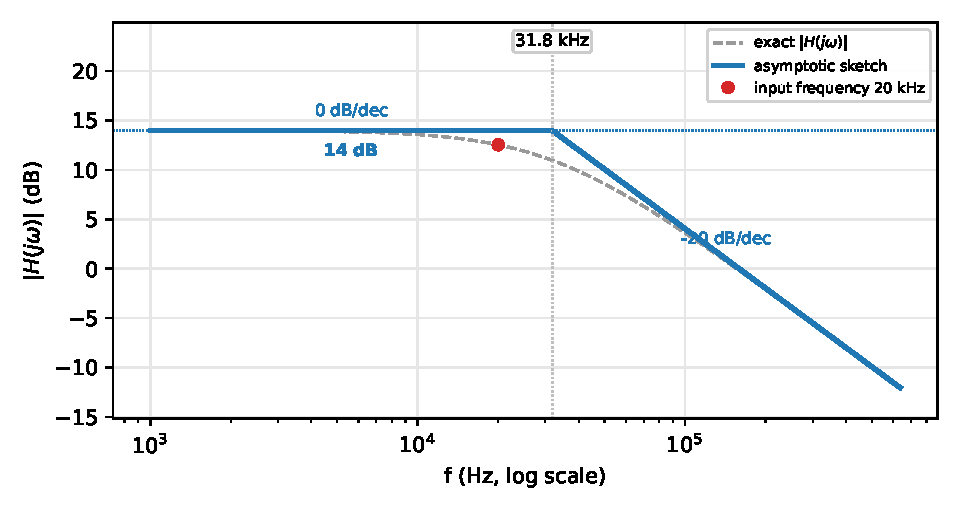
\includegraphics[width=0.78\linewidth,height=6.5cm,keepaspectratio]{p11_bode}\end{center}

{\small Blue: the straight-line sketch you are expected to draw. Dashed grey: the exact curve (about 3\,dB below the corner of an isolated pole). Red dot: the input frequency of Step 7.}
\solstep{7}{Steady-state output}The input is $V_i(t) = 0.2\sin\left(2\pi\cdot 20000\,t\right)$, so $\omega_{in} = 2\pi\cdot 20000 = 1.26\times 10^{5}$\,rad/s. Put $s=j\omega_{in}$ in each factor (tool T5): magnitudes multiply, angles add.
{\small Rules: $\left|\frac{s}{s+p}\right| = \frac{\omega}{\sqrt{\omega^2+p^2}}$, $\angle = \frac{\pi}{2}-\tan^{-1}\frac{\omega}{p}$;\quad $\left|\frac{1}{1+s/p}\right| = \frac{1}{\sqrt{1+(\omega/p)^2}}$, $\angle = -\tan^{-1}\frac{\omega}{p}$;\quad $\left|1+\frac{s}{z}\right| = \sqrt{1+(\omega/z)^2}$, $\angle = \tan^{-1}\frac{\omega}{z}$;\quad a negative $K$ adds $-\pi$.}
\begin{center}\renewcommand{\arraystretch}{1.35}
\begin{tabular}{ccc}
\toprule
factor & magnitude & angle (rad) \\
\midrule
$5$ & $5$ & $0$ \\
$\rule[-1.7em]{0pt}{4em}\dfrac{1}{1+\dfrac{s}{2\pi\cdot 31.8\mathrm{k}}}$ & $0.8467$ & $-0.561$ \\
\textbf{total} & $\mathbf{4.234}$ (product) & $\mathbf{-0.561}$ (sum) \\
\bottomrule
\end{tabular}\end{center}

\begin{align*}
|H(j\omega_{in})| &= 4.23, \qquad \angle H(j\omega_{in}) = -0.561\ \mathrm{rad} \\
v_{o,ac}(t) &= 4.23\times 0.2\,\sin\left(2\pi\cdot 20000\,t - 0.561\right) = 0.847\,\sin\left(2\pi\cdot 20000\,t - 0.561\right)
\end{align*}

\[
\boxed{V_o(t) = 0.847\,\sin\left(2\pi\cdot 20000\,t - 0.561\right)\ \mathrm{V}}
\]

\begin{ansbox}
$H(s) = 5\,\dfrac{1}{1+\dfrac{s}{2\pi\cdot 31.8\mathrm{k}}}$\quad (corners: 31.8 kHz)\\[4pt]
$V_o(t) = 0.847\,\sin\left(2\pi\cdot 20000\,t - 0.561\right)\ \mathrm{V}$
\end{ansbox}

\newpage
\subsection*{Solution 1C.12 \hfill Medium}
\begin{center}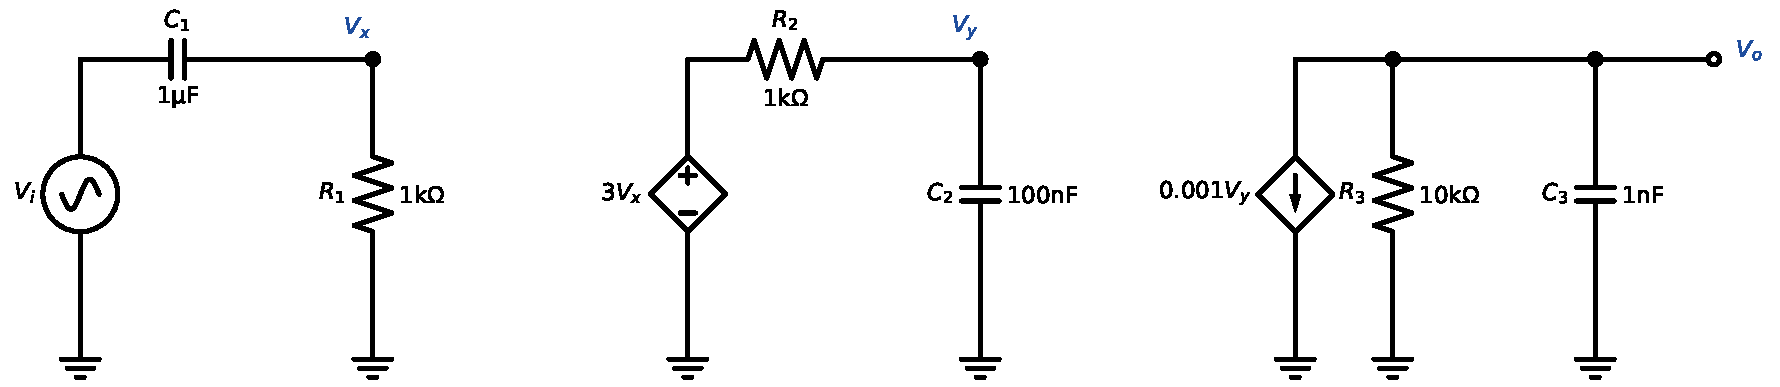
\includegraphics[width=0.8\linewidth,height=4.5cm,keepaspectratio]{p12_circuit}\end{center}
\solstep{1}{Identify the sources}Independent sources: the AC input $V_i(t)$. The diamond-shaped sources are \emph{dependent} sources: they are not inputs, they only copy/scale a voltage that already exists in the circuit, so they stay in the circuit in every step. There is no DC source, so $V_{o,dc}=0$ and $V_o(t)=v_{o,ac}(t)$: Step 2 is skipped.
\solstep{2}{DC circuit}No DC sources: $V_{o,dc}=0$.
\solstep{3}{AC circuit}Replace every capacitor by $\frac{1}{sC}$ and every inductor by $sL$.
AC equivalent circuit (nodes named for the next step):
\begin{center}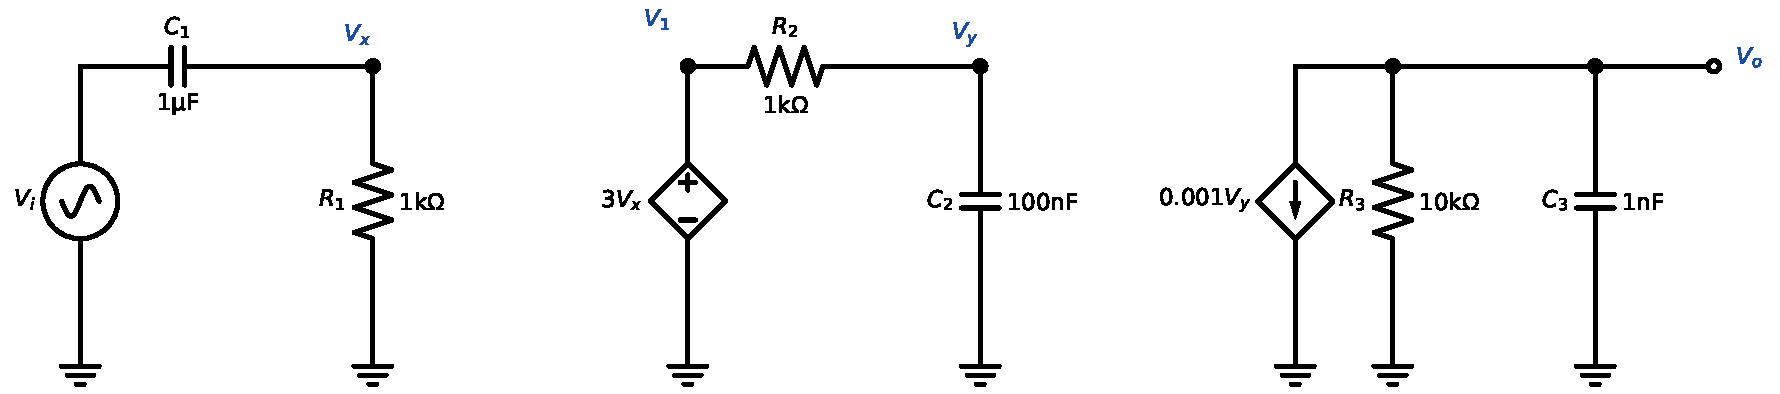
\includegraphics[width=0.95\linewidth,height=5.2cm,keepaspectratio]{p12_ac}\end{center}

\solstep{4}{Transfer function by a chain of dividers}Walk from the input to the output through the named nodes: $V_{i} \to V_{x} \to V_{1} \to V_{y} \to V_{o}$. The transfer function is the product of the node-to-node ratios (each one is a simple divider, tool T2, or a dependent source, tool T4):
\[
H(s) = \frac{V_o}{V_i} = \frac{V_{x}}{V_{i}}\cdot\frac{V_{1}}{V_{x}}\cdot\frac{V_{y}}{V_{1}}\cdot\frac{V_{o}}{V_{y}}
\]

Impedances seen \emph{looking right} from a node (everything from that node to ground, excluding what is on its left). Compute them from the far right toward the input:
\begin{align*}
Z_{o} &= R_{3} \parallel \frac{1}{sC_{3}} = \dfrac{10^{9}}{s + 10^{5}}
\end{align*}

Now each link. {\small (Algebra tip: to simplify a fraction that contains fractions, multiply its top and bottom by every inner denominator; then divide top and bottom by the leading coefficient of the denominator so that it starts with a plain $s^n$.)}
\begin{align*}
\frac{V_{x}}{V_{i}} &= \frac{R_{1}}{\frac{1}{sC_{1}} + R_{1}} = \dfrac{s}{s + 1000} \\
\frac{V_{1}}{V_{x}} &= 3 &&\text{(ideal VCVS: $V_{1} = 3V_{x}$)} \\
\frac{V_{y}}{V_{1}} &= \frac{\frac{1}{sC_{2}}}{R_{2} + \frac{1}{sC_{2}}} = \dfrac{10000}{s + 10000} \\
\frac{V_{o}}{V_{y}} &= -0.001\,Z_{o} = \dfrac{-10^{6}}{s + 10^{5}}
\end{align*}

(VCCS: the current $0.001V_{y}$ flows out of node $V_{o}$ and through $Z_{o}$ to ground, so $V_{o} = -0.001V_{y}\,Z_{o}$ by Ohm's law.)
Multiply the links and simplify (common factors cancel):\[
H(s) = \dfrac{-3\times 10^{10}\,s}{s^{3} + 1.11\times 10^{5}\,s^{2} + 1.11\times 10^{9}\,s + 10^{12}}
\]

\solstep{5}{Standard (Bode-ready) form}Find the roots. Every root $s=-p$ of the denominator is a \emph{pole}, every root $s=-z$ of the numerator is a \emph{zero}; $|p|$ and $|z|$ are the corner frequencies (rad/s).
\begin{itemize}[leftmargin=*,itemsep=2pt]
\item Numerator: it has the factor $s$ $\Rightarrow$ 1 zero at $s=0$.
\item Denominator: $s^{3} + 1.11\times 10^{5}\,s^{2} + 1.11\times 10^{9}\,s + 10^{12}$; this is degree 3: use a calculator's polynomial solver (or \texttt{numpy.roots}) $\Rightarrow s = -1000,\ -10000,\ -100000$.
\end{itemize}

Factored form (leading coefficient in front):
\[
H(s) = -3\times 10^{10}\,\dfrac{s}{(s+1000)(s+10000)(s+10^{5})}
\]

Bode-ready form: rewrite every $(s+p) = p\left(1+\frac{s}{p}\right)$ and $(s+z) = z\left(1+\frac{s}{z}\right)$, and collect all constants into $K$. Each $s$ in the numerator is paired with one of the \emph{lowest} poles as $\frac{s}{s+p}$ (that factor is $\approx 1$ above $p$). Then every factor except $K$ is $\approx 1$ inside the pass-band:
\[
H(s) = -30\,\dfrac{s}{s+2\pi\cdot 159}\,\dfrac{1}{1+\dfrac{s}{2\pi\cdot 1.59\mathrm{k}}}\,\dfrac{1}{1+\dfrac{s}{2\pi\cdot 15.9\mathrm{k}}},\qquad K = -30
\]

\begin{center}\renewcommand{\arraystretch}{1.35}
\begin{tabular}{cccc}
\toprule
type & $\omega_c$ (rad/s) & $f_c=\omega_c/2\pi$ & slope change \\
\midrule
pole & $1000$ & 159 Hz & $-20$ dB/dec \\
pole & $10000$ & 1.59 kHz & $-20$ dB/dec \\
pole & $10^{5}$ & 15.9 kHz & $-20$ dB/dec \\
\bottomrule
\end{tabular}\end{center}

\solstep{6}{Magnitude Bode plot}Below every corner $|H(s)|\approx 0.03\,s$, so the plot starts with a slope of $+20$\,dB/dec. Then, moving right, each pole bends the line down by 20\,dB/dec and each zero bends it up by 20\,dB/dec (tool T6):
\begin{center}\renewcommand{\arraystretch}{1.35}
\begin{tabular}{lcl}
\toprule
frequency range & slope & asymptote level \\
\midrule
$f<$ 159 Hz & $+20$ dB/dec & 29.5 dB at end \\
159 Hz -- 1.59 kHz & $0$ dB/dec (flat) & 29.5 dB at start, 29.5 dB at end \\
1.59 kHz -- 15.9 kHz & $-20$ dB/dec & 29.5 dB at start, 9.54 dB at end \\
$f>$ 15.9 kHz & $-40$ dB/dec & 9.54 dB at start \\
\bottomrule
\end{tabular}\end{center}

The flat (pass-band) level is $20\log_{10}|K| = 20\log_{10}30 = 29.5$\,dB.
\begin{center}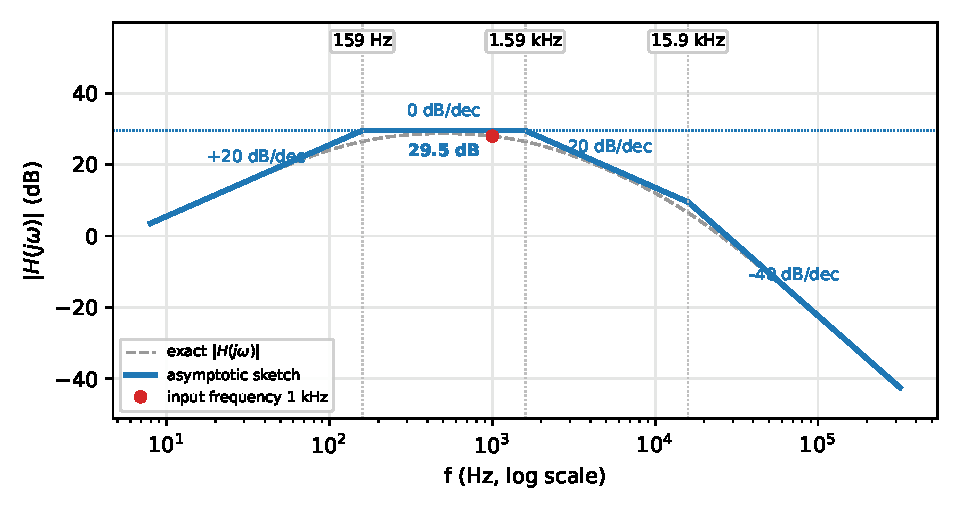
\includegraphics[width=0.78\linewidth,height=6.5cm,keepaspectratio]{p12_bode}\end{center}

{\small Blue: the straight-line sketch you are expected to draw. Dashed grey: the exact curve (about 3\,dB below the corner of an isolated pole). Red dot: the input frequency of Step 7.}
\solstep{7}{Steady-state output}The input is $V_i(t) = 0.1\sin\left(2\pi\cdot 1000\,t\right)$, so $\omega_{in} = 2\pi\cdot 1000 = 6280$\,rad/s. Put $s=j\omega_{in}$ in each factor (tool T5): magnitudes multiply, angles add.
{\small Rules: $\left|\frac{s}{s+p}\right| = \frac{\omega}{\sqrt{\omega^2+p^2}}$, $\angle = \frac{\pi}{2}-\tan^{-1}\frac{\omega}{p}$;\quad $\left|\frac{1}{1+s/p}\right| = \frac{1}{\sqrt{1+(\omega/p)^2}}$, $\angle = -\tan^{-1}\frac{\omega}{p}$;\quad $\left|1+\frac{s}{z}\right| = \sqrt{1+(\omega/z)^2}$, $\angle = \tan^{-1}\frac{\omega}{z}$;\quad a negative $K$ adds $-\pi$.}
\begin{center}\renewcommand{\arraystretch}{1.35}
\begin{tabular}{ccc}
\toprule
factor & magnitude & angle (rad) \\
\midrule
$-30$ & $30$ & $-3.14$ \\
$\rule[-1.1em]{0pt}{2.8em}\dfrac{s}{s+2\pi\cdot 159}$ & $0.9876$ & $0.158$ \\
$\rule[-1.7em]{0pt}{4em}\dfrac{1}{1+\dfrac{s}{2\pi\cdot 1.59\mathrm{k}}}$ & $0.8467$ & $-0.561$ \\
$\rule[-1.7em]{0pt}{4em}\dfrac{1}{1+\dfrac{s}{2\pi\cdot 15.9\mathrm{k}}}$ & $0.998$ & $-0.0627$ \\
\textbf{total} & $\mathbf{25.04}$ (product) & $\mathbf{-3.61}$ (sum) \\
\bottomrule
\end{tabular}\end{center}

\begin{align*}
|H(j\omega_{in})| &= 25, \qquad \angle H(j\omega_{in}) = -3.61\ \mathrm{rad} \\
v_{o,ac}(t) &= 25\times 0.1\,\sin\left(2\pi\cdot 1000\,t - 3.61\right) = 2.5\,\sin\left(2\pi\cdot 1000\,t - 3.61\right)
\end{align*}

\[
\boxed{V_o(t) = 2.5\,\sin\left(2\pi\cdot 1000\,t - 3.61\right)\ \mathrm{V}}
\]

\begin{ansbox}
$H(s) = -30\,\dfrac{s}{s+2\pi\cdot 159}\,\dfrac{1}{1+\dfrac{s}{2\pi\cdot 1.59\mathrm{k}}}\,\dfrac{1}{1+\dfrac{s}{2\pi\cdot 15.9\mathrm{k}}}$\quad (corners: 159 Hz, 1.59 kHz, 15.9 kHz)\\[4pt]
$V_o(t) = 2.5\,\sin\left(2\pi\cdot 1000\,t - 3.61\right)\ \mathrm{V}$
\end{ansbox}

\newpage
\subsection*{Solution 1C.13 \hfill Hard}
\begin{center}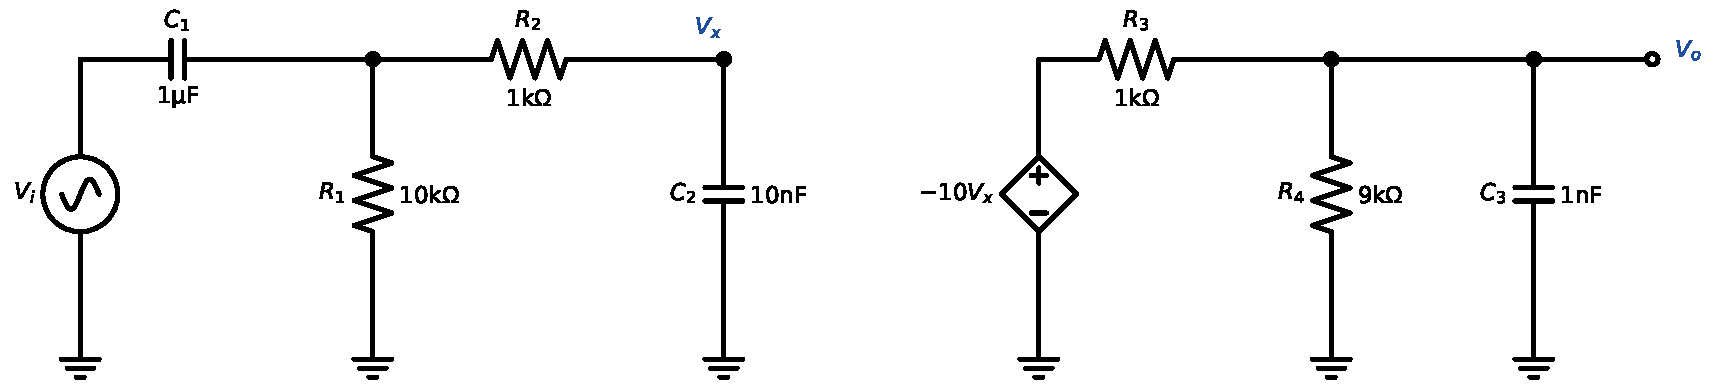
\includegraphics[width=0.8\linewidth,height=4.5cm,keepaspectratio]{p13_circuit}\end{center}
\solstep{1}{Identify the sources}Independent sources: the AC input $V_i(t)$. The diamond-shaped sources are \emph{dependent} sources: they are not inputs, they only copy/scale a voltage that already exists in the circuit, so they stay in the circuit in every step. There is no DC source, so $V_{o,dc}=0$ and $V_o(t)=v_{o,ac}(t)$: Step 2 is skipped.
\solstep{2}{DC circuit}No DC sources: $V_{o,dc}=0$.
\solstep{3}{AC circuit}Replace every capacitor by $\frac{1}{sC}$ and every inductor by $sL$.
AC equivalent circuit (nodes named for the next step):
\begin{center}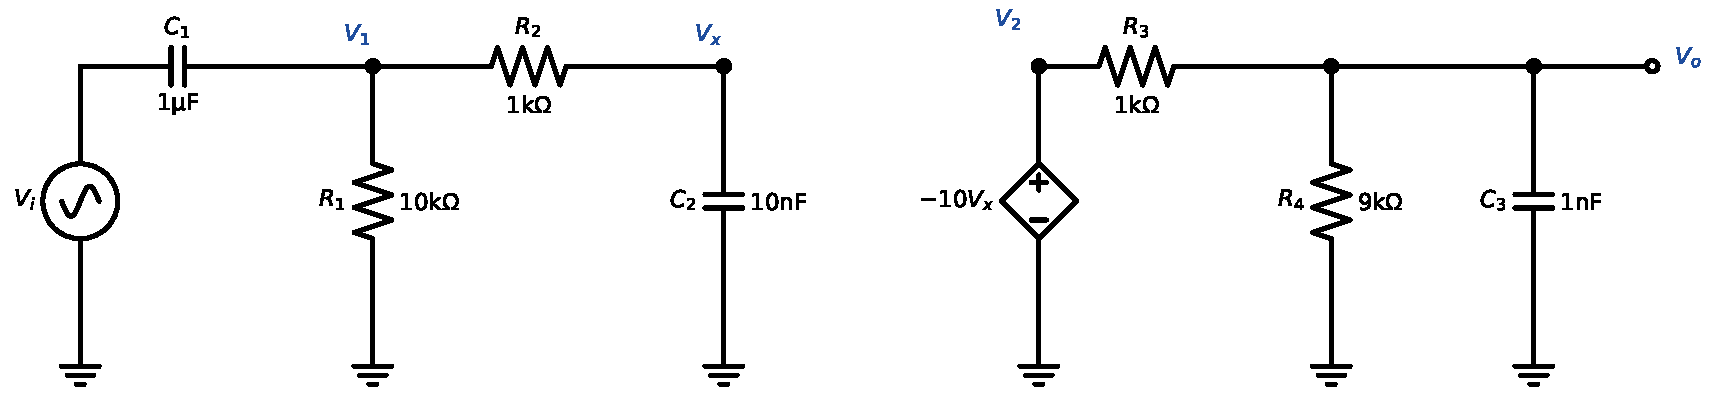
\includegraphics[width=0.95\linewidth,height=5.2cm,keepaspectratio]{p13_ac}\end{center}

\solstep{4}{Transfer function by a chain of dividers}Walk from the input to the output through the named nodes: $V_{i} \to V_{1} \to V_{x} \to V_{2} \to V_{o}$. The transfer function is the product of the node-to-node ratios (each one is a simple divider, tool T2, or a dependent source, tool T4):
\[
H(s) = \frac{V_o}{V_i} = \frac{V_{1}}{V_{i}}\cdot\frac{V_{x}}{V_{1}}\cdot\frac{V_{2}}{V_{x}}\cdot\frac{V_{o}}{V_{2}}
\]

Impedances seen \emph{looking right} from a node (everything from that node to ground, excluding what is on its left). Compute them from the far right toward the input:
\begin{align*}
Z_{1} &= R_{1} \parallel \left(R_{2} + \frac{1}{sC_{2}}\right) = \dfrac{909\,s + 9.09\times 10^{7}}{s + 9090} \\
Z_{o} &= R_{4} \parallel \frac{1}{sC_{3}} = \dfrac{10^{9}}{s + 1.11\times 10^{5}}
\end{align*}

Now each link. {\small (Algebra tip: to simplify a fraction that contains fractions, multiply its top and bottom by every inner denominator; then divide top and bottom by the leading coefficient of the denominator so that it starts with a plain $s^n$.)}
\begin{align*}
\frac{V_{1}}{V_{i}} &= \frac{Z_{1}}{\frac{1}{sC_{1}} + Z_{1}} = \dfrac{s^{2} + 10^{5}\,s}{s^{2} + 1.01\times 10^{5}\,s + 10^{7}} \\
\frac{V_{x}}{V_{1}} &= \frac{\frac{1}{sC_{2}}}{R_{2} + \frac{1}{sC_{2}}} = \dfrac{10^{5}}{s + 10^{5}} \\
\frac{V_{2}}{V_{x}} &= -10 &&\text{(ideal VCVS: $V_{2} = -10V_{x}$)} \\
\frac{V_{o}}{V_{2}} &= \frac{Z_{o}}{R_{3} + Z_{o}} = \dfrac{10^{6}}{s + 1.11\times 10^{6}}
\end{align*}

Multiply the links and simplify (common factors cancel):\[
H(s) = \dfrac{-10^{12}\,s}{s^{3} + 1.21\times 10^{6}\,s^{2} + 1.12\times 10^{11}\,s + 1.11\times 10^{13}}
\]

\solstep{5}{Standard (Bode-ready) form}Find the roots. Every root $s=-p$ of the denominator is a \emph{pole}, every root $s=-z$ of the numerator is a \emph{zero}; $|p|$ and $|z|$ are the corner frequencies (rad/s).
\begin{itemize}[leftmargin=*,itemsep=2pt]
\item Numerator: it has the factor $s$ $\Rightarrow$ 1 zero at $s=0$.
\item Denominator: $s^{3} + 1.21\times 10^{6}\,s^{2} + 1.12\times 10^{11}\,s + 1.11\times 10^{13}$; this is degree 3: use a calculator's polynomial solver (or \texttt{numpy.roots}) $\Rightarrow s = -99,\ -1.01\times 10^{5},\ -1.11\times 10^{6}$.
\end{itemize}

Factored form (leading coefficient in front):
\[
H(s) = -10^{12}\,\dfrac{s}{(s+99)(s+1.01\times 10^{5})(s+1.11\times 10^{6})}
\]

Bode-ready form: rewrite every $(s+p) = p\left(1+\frac{s}{p}\right)$ and $(s+z) = z\left(1+\frac{s}{z}\right)$, and collect all constants into $K$. Each $s$ in the numerator is paired with one of the \emph{lowest} poles as $\frac{s}{s+p}$ (that factor is $\approx 1$ above $p$). Then every factor except $K$ is $\approx 1$ inside the pass-band:
\[
H(s) = -8.91\,\dfrac{s}{s+2\pi\cdot 15.8}\,\dfrac{1}{1+\dfrac{s}{2\pi\cdot 16.1\mathrm{k}}}\,\dfrac{1}{1+\dfrac{s}{2\pi\cdot 177\mathrm{k}}},\qquad K = -8.91
\]

\begin{center}\renewcommand{\arraystretch}{1.35}
\begin{tabular}{cccc}
\toprule
type & $\omega_c$ (rad/s) & $f_c=\omega_c/2\pi$ & slope change \\
\midrule
pole & $99$ & 15.8 Hz & $-20$ dB/dec \\
pole & $1.01\times 10^{5}$ & 16.1 kHz & $-20$ dB/dec \\
pole & $1.11\times 10^{6}$ & 177 kHz & $-20$ dB/dec \\
\bottomrule
\end{tabular}\end{center}

\solstep{6}{Magnitude Bode plot}Below every corner $|H(s)|\approx 0.09\,s$, so the plot starts with a slope of $+20$\,dB/dec. Then, moving right, each pole bends the line down by 20\,dB/dec and each zero bends it up by 20\,dB/dec (tool T6):
\begin{center}\renewcommand{\arraystretch}{1.35}
\begin{tabular}{lcl}
\toprule
frequency range & slope & asymptote level \\
\midrule
$f<$ 15.8 Hz & $+20$ dB/dec & 19 dB at end \\
15.8 Hz -- 16.1 kHz & $0$ dB/dec (flat) & 19 dB at start, 19 dB at end \\
16.1 kHz -- 177 kHz & $-20$ dB/dec & 19 dB at start, -1.83 dB at end \\
$f>$ 177 kHz & $-40$ dB/dec & -1.83 dB at start \\
\bottomrule
\end{tabular}\end{center}

The flat (pass-band) level is $20\log_{10}|K| = 20\log_{10}8.91 = 19$\,dB.
\begin{center}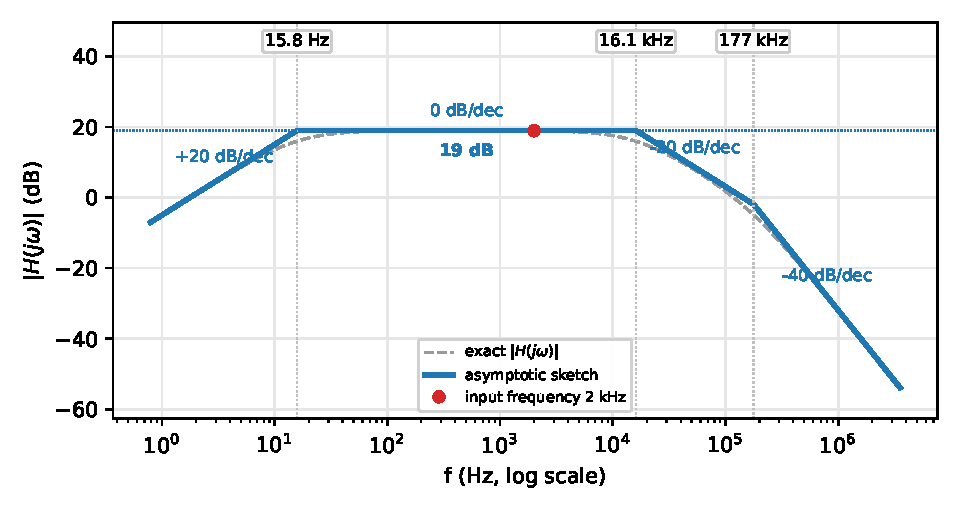
\includegraphics[width=0.78\linewidth,height=6.5cm,keepaspectratio]{p13_bode}\end{center}

{\small Blue: the straight-line sketch you are expected to draw. Dashed grey: the exact curve (about 3\,dB below the corner of an isolated pole). Red dot: the input frequency of Step 7.}
\solstep{7}{Steady-state output}The input is $V_i(t) = 0.05\sin\left(2\pi\cdot 2000\,t\right)$, so $\omega_{in} = 2\pi\cdot 2000 = 12600$\,rad/s. Put $s=j\omega_{in}$ in each factor (tool T5): magnitudes multiply, angles add.
{\small Rules: $\left|\frac{s}{s+p}\right| = \frac{\omega}{\sqrt{\omega^2+p^2}}$, $\angle = \frac{\pi}{2}-\tan^{-1}\frac{\omega}{p}$;\quad $\left|\frac{1}{1+s/p}\right| = \frac{1}{\sqrt{1+(\omega/p)^2}}$, $\angle = -\tan^{-1}\frac{\omega}{p}$;\quad $\left|1+\frac{s}{z}\right| = \sqrt{1+(\omega/z)^2}$, $\angle = \tan^{-1}\frac{\omega}{z}$;\quad a negative $K$ adds $-\pi$.}
\begin{center}\renewcommand{\arraystretch}{1.35}
\begin{tabular}{ccc}
\toprule
factor & magnitude & angle (rad) \\
\midrule
$-8.91$ & $8.911$ & $-3.14$ \\
$\rule[-1.1em]{0pt}{2.8em}\dfrac{s}{s+2\pi\cdot 15.8}$ & $1$ & $0.00788$ \\
$\rule[-1.7em]{0pt}{4em}\dfrac{1}{1+\dfrac{s}{2\pi\cdot 16.1\mathrm{k}}}$ & $0.9923$ & $-0.124$ \\
$\rule[-1.7em]{0pt}{4em}\dfrac{1}{1+\dfrac{s}{2\pi\cdot 177\mathrm{k}}}$ & $0.9999$ & $-0.0113$ \\
\textbf{total} & $\mathbf{8.842}$ (product) & $\mathbf{-3.27}$ (sum) \\
\bottomrule
\end{tabular}\end{center}

\begin{align*}
|H(j\omega_{in})| &= 8.84, \qquad \angle H(j\omega_{in}) = -3.27\ \mathrm{rad} \\
v_{o,ac}(t) &= 8.84\times 0.05\,\sin\left(2\pi\cdot 2000\,t - 3.27\right) = 0.442\,\sin\left(2\pi\cdot 2000\,t - 3.27\right)
\end{align*}

\[
\boxed{V_o(t) = 0.442\,\sin\left(2\pi\cdot 2000\,t - 3.27\right)\ \mathrm{V}}
\]

\begin{ansbox}
$H(s) = -8.91\,\dfrac{s}{s+2\pi\cdot 15.8}\,\dfrac{1}{1+\dfrac{s}{2\pi\cdot 16.1\mathrm{k}}}\,\dfrac{1}{1+\dfrac{s}{2\pi\cdot 177\mathrm{k}}}$\quad (corners: 15.8 Hz, 16.1 kHz, 177 kHz)\\[4pt]
$V_o(t) = 0.442\,\sin\left(2\pi\cdot 2000\,t - 3.27\right)\ \mathrm{V}$
\end{ansbox}

\newpage
\subsection*{Solution 1C.14 \hfill Hard}
\begin{center}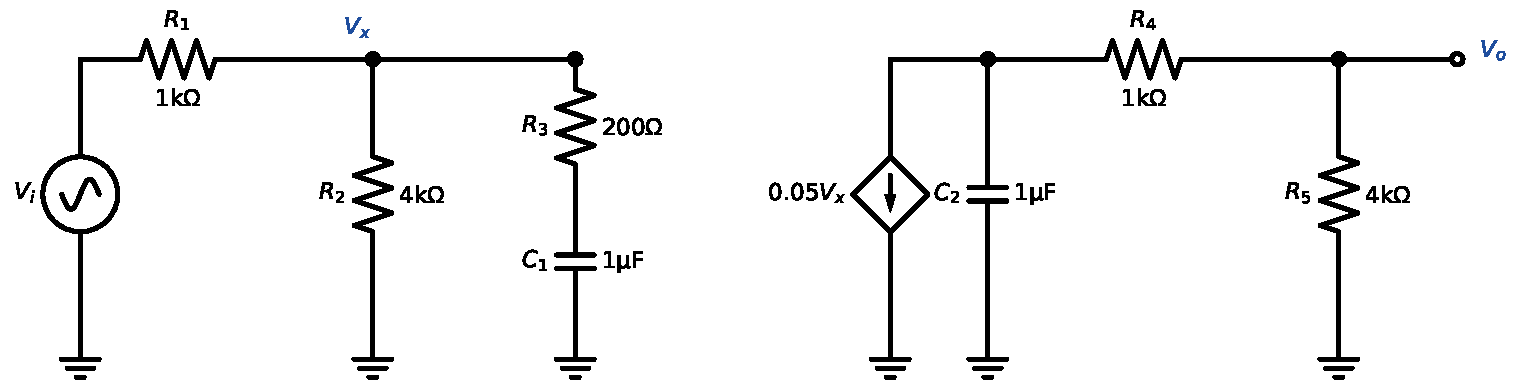
\includegraphics[width=0.8\linewidth,height=4.5cm,keepaspectratio]{p14_circuit}\end{center}
\solstep{1}{Identify the sources}Independent sources: the AC input $V_i(t)$. The diamond-shaped sources are \emph{dependent} sources: they are not inputs, they only copy/scale a voltage that already exists in the circuit, so they stay in the circuit in every step. There is no DC source, so $V_{o,dc}=0$ and $V_o(t)=v_{o,ac}(t)$: Step 2 is skipped.
\solstep{2}{DC circuit}No DC sources: $V_{o,dc}=0$.
\solstep{3}{AC circuit}Replace every capacitor by $\frac{1}{sC}$ and every inductor by $sL$.
AC equivalent circuit (nodes named for the next step):
\begin{center}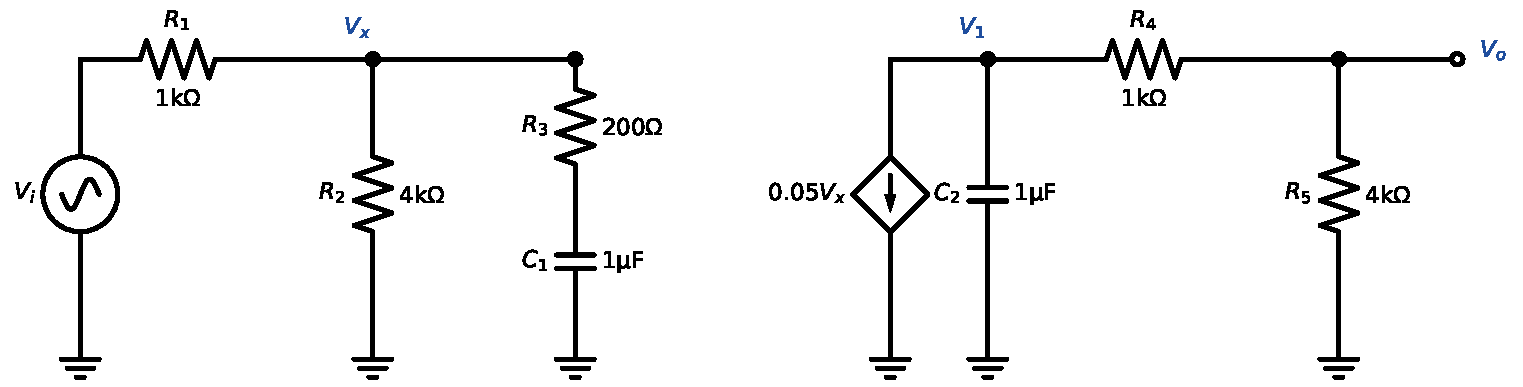
\includegraphics[width=0.95\linewidth,height=5.2cm,keepaspectratio]{p14_ac}\end{center}

\solstep{4}{Transfer function by a chain of dividers}Walk from the input to the output through the named nodes: $V_{i} \to V_{x} \to V_{1} \to V_{o}$. The transfer function is the product of the node-to-node ratios (each one is a simple divider, tool T2, or a dependent source, tool T4):
\[
H(s) = \frac{V_o}{V_i} = \frac{V_{x}}{V_{i}}\cdot\frac{V_{1}}{V_{x}}\cdot\frac{V_{o}}{V_{1}}
\]

Impedances seen \emph{looking right} from a node (everything from that node to ground, excluding what is on its left). Compute them from the far right toward the input:
\begin{align*}
Z_{x} &= R_{2} \parallel \left(R_{3} + \frac{1}{sC_{1}}\right) = \dfrac{190\,s + 9.52\times 10^{5}}{s + 238} \\
Z_{1} &= \frac{1}{sC_{2}} \parallel \left(R_{4} + R_{5}\right) = \dfrac{10^{6}}{s + 200}
\end{align*}

Now each link. {\small (Algebra tip: to simplify a fraction that contains fractions, multiply its top and bottom by every inner denominator; then divide top and bottom by the leading coefficient of the denominator so that it starts with a plain $s^n$.)}
\begin{align*}
\frac{V_{x}}{V_{i}} &= \frac{Z_{x}}{R_{1} + Z_{x}} = \dfrac{0.16\,s + 800}{s + 1000} \\
\frac{V_{1}}{V_{x}} &= -0.05\,Z_{1} = \dfrac{-50000}{s + 200} \\
\frac{V_{o}}{V_{1}} &= \frac{R_{5}}{R_{4} + R_{5}} = 0.8
\end{align*}

(VCCS: the current $0.05V_{x}$ flows out of node $V_{1}$ and through $Z_{1}$ to ground, so $V_{1} = -0.05V_{x}\,Z_{1}$ by Ohm's law.)
Multiply the links and simplify (common factors cancel):\[
H(s) = \dfrac{-6400\,s - 3.2\times 10^{7}}{s^{2} + 1200\,s + 2\times 10^{5}}
\]

\solstep{5}{Standard (Bode-ready) form}Find the roots. Every root $s=-p$ of the denominator is a \emph{pole}, every root $s=-z$ of the numerator is a \emph{zero}; $|p|$ and $|z|$ are the corner frequencies (rad/s).
\begin{itemize}[leftmargin=*,itemsep=2pt]
\item Numerator: $-6400\,s - 3.2\times 10^{7}$; divide by the leading coefficient $-6400$ (this does not move the roots): $s + 5000$; $s + 5000 = 0 \Rightarrow s = -5000$.
\item Denominator: $s^{2} + 1200\,s + 2\times 10^{5}$; quadratic formula:\[
s = \frac{-1200 \pm \sqrt{(1200)^2 - 4(2\times 10^{5})}}{2} = \frac{-1200 \pm 800}{2} \Rightarrow s = -200,\ -1000
\]

\end{itemize}

Factored form (leading coefficient in front):
\[
H(s) = -6400\,\dfrac{(s+5000)}{(s+200)(s+1000)}
\]

Bode-ready form: rewrite every $(s+p) = p\left(1+\frac{s}{p}\right)$ and $(s+z) = z\left(1+\frac{s}{z}\right)$, and collect all constants into $K$. Then every factor except $K$ is $\approx 1$ inside the pass-band:
\[
H(s) = -160\,\dfrac{1}{1+\dfrac{s}{2\pi\cdot 31.8}}\,\dfrac{1}{1+\dfrac{s}{2\pi\cdot 159}}\,\left(1+\dfrac{s}{2\pi\cdot 796}\right),\qquad K = -160
\]

\begin{center}\renewcommand{\arraystretch}{1.35}
\begin{tabular}{cccc}
\toprule
type & $\omega_c$ (rad/s) & $f_c=\omega_c/2\pi$ & slope change \\
\midrule
pole & $200$ & 31.8 Hz & $-20$ dB/dec \\
pole & $1000$ & 159 Hz & $-20$ dB/dec \\
zero & $5000$ & 796 Hz & $+20$ dB/dec \\
\bottomrule
\end{tabular}\end{center}

\solstep{6}{Magnitude Bode plot}Below every corner, all factors are $\approx$ constant: $|H| \approx 160$ $= 44.1$\,dB (flat, 0 dB/dec). Then, moving right, each pole bends the line down by 20\,dB/dec and each zero bends it up by 20\,dB/dec (tool T6):
\begin{center}\renewcommand{\arraystretch}{1.35}
\begin{tabular}{lcl}
\toprule
frequency range & slope & asymptote level \\
\midrule
$f<$ 31.8 Hz & $0$ dB/dec (flat) & 44.1 dB at end \\
31.8 Hz -- 159 Hz & $-20$ dB/dec & 44.1 dB at start, 30.1 dB at end \\
159 Hz -- 796 Hz & $-40$ dB/dec & 30.1 dB at start, 2.14 dB at end \\
$f>$ 796 Hz & $-20$ dB/dec & 2.14 dB at start \\
\bottomrule
\end{tabular}\end{center}

\begin{center}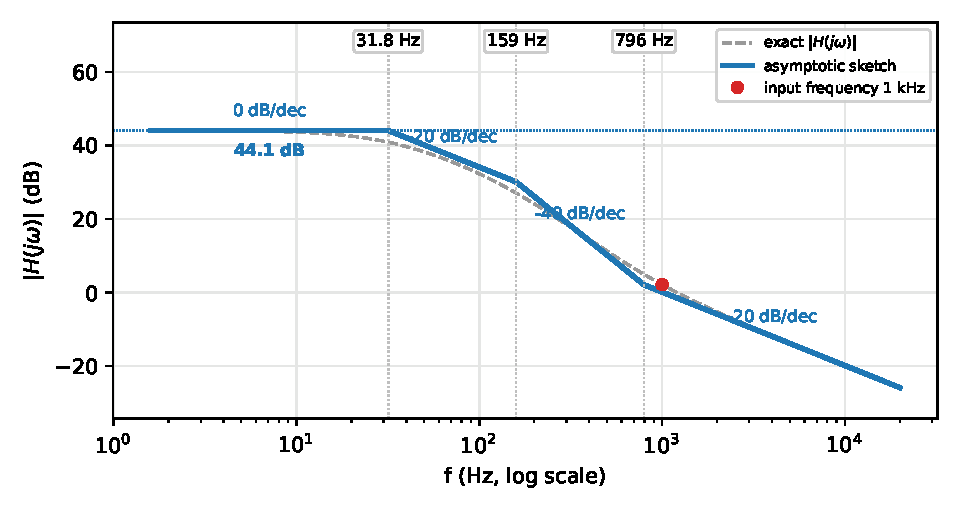
\includegraphics[width=0.78\linewidth,height=6.5cm,keepaspectratio]{p14_bode}\end{center}

{\small Blue: the straight-line sketch you are expected to draw. Dashed grey: the exact curve (about 3\,dB below the corner of an isolated pole). Red dot: the input frequency of Step 7.}
\solstep{7}{Steady-state output}The input is $V_i(t) = 0.02\sin\left(2\pi\cdot 1000\,t\right)$, so $\omega_{in} = 2\pi\cdot 1000 = 6280$\,rad/s. Put $s=j\omega_{in}$ in each factor (tool T5): magnitudes multiply, angles add.
{\small Rules: $\left|\frac{s}{s+p}\right| = \frac{\omega}{\sqrt{\omega^2+p^2}}$, $\angle = \frac{\pi}{2}-\tan^{-1}\frac{\omega}{p}$;\quad $\left|\frac{1}{1+s/p}\right| = \frac{1}{\sqrt{1+(\omega/p)^2}}$, $\angle = -\tan^{-1}\frac{\omega}{p}$;\quad $\left|1+\frac{s}{z}\right| = \sqrt{1+(\omega/z)^2}$, $\angle = \tan^{-1}\frac{\omega}{z}$;\quad a negative $K$ adds $-\pi$.}
\begin{center}\renewcommand{\arraystretch}{1.35}
\begin{tabular}{ccc}
\toprule
factor & magnitude & angle (rad) \\
\midrule
$-160$ & $160$ & $-3.14$ \\
$\rule[-1.7em]{0pt}{4em}\dfrac{1}{1+\dfrac{s}{2\pi\cdot 31.8}}$ & $0.03181$ & $-1.54$ \\
$\rule[-1.7em]{0pt}{4em}\dfrac{1}{1+\dfrac{s}{2\pi\cdot 159}}$ & $0.1572$ & $-1.41$ \\
$\rule[-1.1em]{0pt}{2.8em}\left(1+\dfrac{s}{2\pi\cdot 796}\right)$ & $1.606$ & $0.899$ \\
\textbf{total} & $\mathbf{1.285}$ (product) & $\mathbf{-5.19}$ (sum) \\
\bottomrule
\end{tabular}\end{center}

\begin{align*}
|H(j\omega_{in})| &= 1.28, \qquad \angle H(j\omega_{in}) = -5.19\ \mathrm{rad} \\
v_{o,ac}(t) &= 1.28\times 0.02\,\sin\left(2\pi\cdot 1000\,t - 5.19\right) = 0.0257\,\sin\left(2\pi\cdot 1000\,t - 5.19\right)
\end{align*}

\[
\boxed{V_o(t) = 0.0257\,\sin\left(2\pi\cdot 1000\,t - 5.19\right)\ \mathrm{V}}
\]

\begin{ansbox}
$H(s) = -160\,\dfrac{1}{1+\dfrac{s}{2\pi\cdot 31.8}}\,\dfrac{1}{1+\dfrac{s}{2\pi\cdot 159}}\,\left(1+\dfrac{s}{2\pi\cdot 796}\right)$\quad (corners: 31.8 Hz, 159 Hz, 796 Hz)\\[4pt]
$V_o(t) = 0.0257\,\sin\left(2\pi\cdot 1000\,t - 5.19\right)\ \mathrm{V}$
\end{ansbox}

\newpage
\subsection*{Solution 1C.15 \hfill Hard}
\begin{center}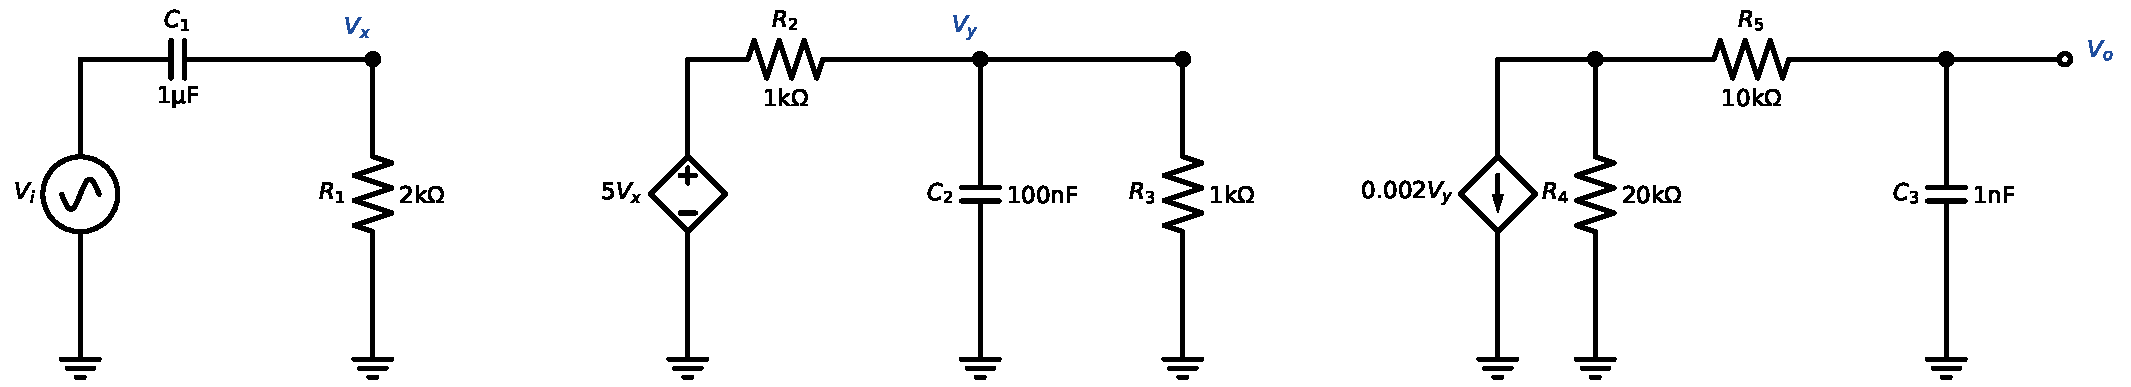
\includegraphics[width=0.8\linewidth,height=4.5cm,keepaspectratio]{p15_circuit}\end{center}
\solstep{1}{Identify the sources}Independent sources: the AC input $V_i(t)$. The diamond-shaped sources are \emph{dependent} sources: they are not inputs, they only copy/scale a voltage that already exists in the circuit, so they stay in the circuit in every step. There is no DC source, so $V_{o,dc}=0$ and $V_o(t)=v_{o,ac}(t)$: Step 2 is skipped.
\solstep{2}{DC circuit}No DC sources: $V_{o,dc}=0$.
\solstep{3}{AC circuit}Replace every capacitor by $\frac{1}{sC}$ and every inductor by $sL$.
AC equivalent circuit (nodes named for the next step):
\begin{center}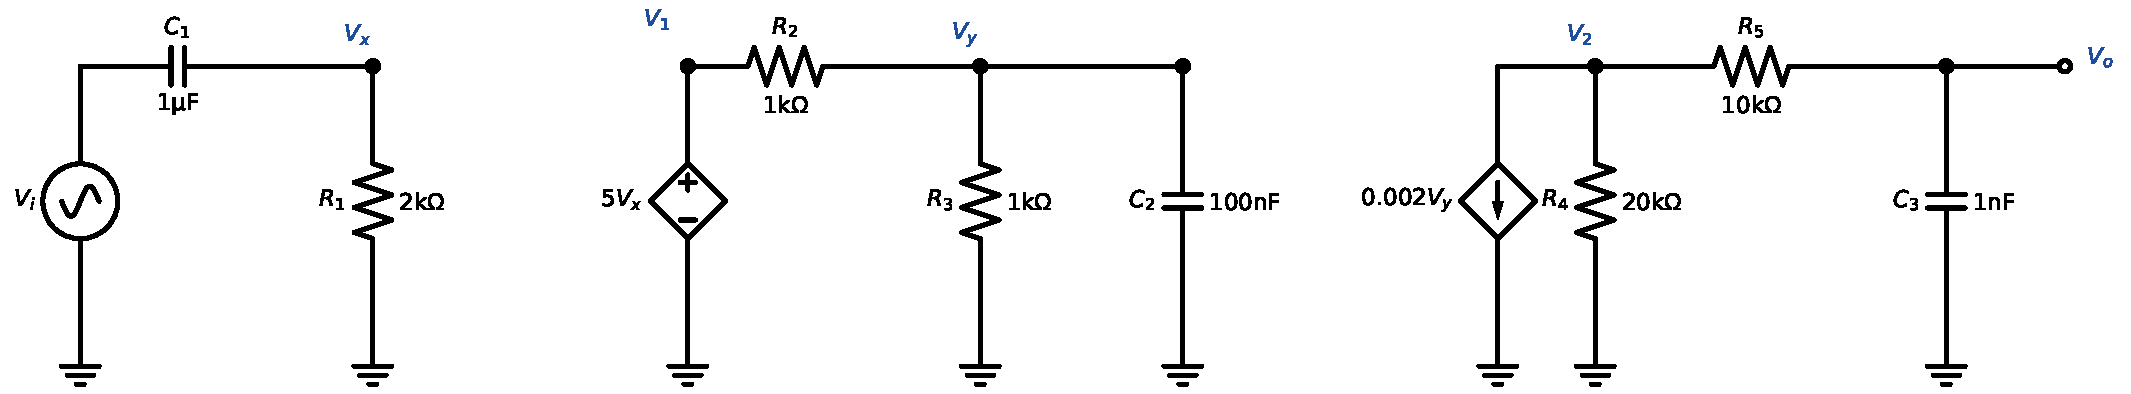
\includegraphics[width=0.95\linewidth,height=5.2cm,keepaspectratio]{p15_ac}\end{center}

\solstep{4}{Transfer function by a chain of dividers}Walk from the input to the output through the named nodes: $V_{i} \to V_{x} \to V_{1} \to V_{y} \to V_{2} \to V_{o}$. The transfer function is the product of the node-to-node ratios (each one is a simple divider, tool T2, or a dependent source, tool T4):
\[
H(s) = \frac{V_o}{V_i} = \frac{V_{x}}{V_{i}}\cdot\frac{V_{1}}{V_{x}}\cdot\frac{V_{y}}{V_{1}}\cdot\frac{V_{2}}{V_{y}}\cdot\frac{V_{o}}{V_{2}}
\]

Impedances seen \emph{looking right} from a node (everything from that node to ground, excluding what is on its left). Compute them from the far right toward the input:
\begin{align*}
Z_{y} &= R_{3} \parallel \frac{1}{sC_{2}} = \dfrac{10^{7}}{s + 10000} \\
Z_{2} &= R_{4} \parallel \left(R_{5} + \frac{1}{sC_{3}}\right) = \dfrac{6670\,s + 6.67\times 10^{8}}{s + 33300}
\end{align*}

Now each link. {\small (Algebra tip: to simplify a fraction that contains fractions, multiply its top and bottom by every inner denominator; then divide top and bottom by the leading coefficient of the denominator so that it starts with a plain $s^n$.)}
\begin{align*}
\frac{V_{x}}{V_{i}} &= \frac{R_{1}}{\frac{1}{sC_{1}} + R_{1}} = \dfrac{s}{s + 500} \\
\frac{V_{1}}{V_{x}} &= 5 &&\text{(ideal VCVS: $V_{1} = 5V_{x}$)} \\
\frac{V_{y}}{V_{1}} &= \frac{Z_{y}}{R_{2} + Z_{y}} = \dfrac{10000}{s + 20000} \\
\frac{V_{2}}{V_{y}} &= -0.002\,Z_{2} = \dfrac{-13.3\,s - 1.33\times 10^{6}}{s + 33300} \\
\frac{V_{o}}{V_{2}} &= \frac{\frac{1}{sC_{3}}}{R_{5} + \frac{1}{sC_{3}}} = \dfrac{10^{5}}{s + 10^{5}}
\end{align*}

(VCCS: the current $0.002V_{y}$ flows out of node $V_{2}$ and through $Z_{2}$ to ground, so $V_{2} = -0.002V_{y}\,Z_{2}$ by Ohm's law.)
Multiply the links and simplify (common factors cancel):\[
H(s) = \dfrac{-6.67\times 10^{10}\,s}{s^{3} + 53800\,s^{2} + 6.93\times 10^{8}\,s + 3.33\times 10^{11}}
\]

\solstep{5}{Standard (Bode-ready) form}Find the roots. Every root $s=-p$ of the denominator is a \emph{pole}, every root $s=-z$ of the numerator is a \emph{zero}; $|p|$ and $|z|$ are the corner frequencies (rad/s).
\begin{itemize}[leftmargin=*,itemsep=2pt]
\item Numerator: it has the factor $s$ $\Rightarrow$ 1 zero at $s=0$.
\item Denominator: $s^{3} + 53800\,s^{2} + 6.93\times 10^{8}\,s + 3.33\times 10^{11}$; this is degree 3: use a calculator's polynomial solver (or \texttt{numpy.roots}) $\Rightarrow s = -500,\ -20000,\ -33300$.
\end{itemize}

Factored form (leading coefficient in front):
\[
H(s) = -6.67\times 10^{10}\,\dfrac{s}{(s+500)(s+20000)(s+33300)}
\]

Bode-ready form: rewrite every $(s+p) = p\left(1+\frac{s}{p}\right)$ and $(s+z) = z\left(1+\frac{s}{z}\right)$, and collect all constants into $K$. Each $s$ in the numerator is paired with one of the \emph{lowest} poles as $\frac{s}{s+p}$ (that factor is $\approx 1$ above $p$). Then every factor except $K$ is $\approx 1$ inside the pass-band:
\[
H(s) = -100\,\dfrac{s}{s+2\pi\cdot 79.6}\,\dfrac{1}{1+\dfrac{s}{2\pi\cdot 3.18\mathrm{k}}}\,\dfrac{1}{1+\dfrac{s}{2\pi\cdot 5.31\mathrm{k}}},\qquad K = -100
\]

\begin{center}\renewcommand{\arraystretch}{1.35}
\begin{tabular}{cccc}
\toprule
type & $\omega_c$ (rad/s) & $f_c=\omega_c/2\pi$ & slope change \\
\midrule
pole & $500$ & 79.6 Hz & $-20$ dB/dec \\
pole & $20000$ & 3.18 kHz & $-20$ dB/dec \\
pole & $33300$ & 5.31 kHz & $-20$ dB/dec \\
\bottomrule
\end{tabular}\end{center}

\solstep{6}{Magnitude Bode plot}Below every corner $|H(s)|\approx 0.2\,s$, so the plot starts with a slope of $+20$\,dB/dec. Then, moving right, each pole bends the line down by 20\,dB/dec and each zero bends it up by 20\,dB/dec (tool T6):
\begin{center}\renewcommand{\arraystretch}{1.35}
\begin{tabular}{lcl}
\toprule
frequency range & slope & asymptote level \\
\midrule
$f<$ 79.6 Hz & $+20$ dB/dec & 40 dB at end \\
79.6 Hz -- 3.18 kHz & $0$ dB/dec (flat) & 40 dB at start, 40 dB at end \\
3.18 kHz -- 5.31 kHz & $-20$ dB/dec & 40 dB at start, 35.6 dB at end \\
$f>$ 5.31 kHz & $-40$ dB/dec & 35.6 dB at start \\
\bottomrule
\end{tabular}\end{center}

The flat (pass-band) level is $20\log_{10}|K| = 20\log_{10}100 = 40$\,dB.
\begin{center}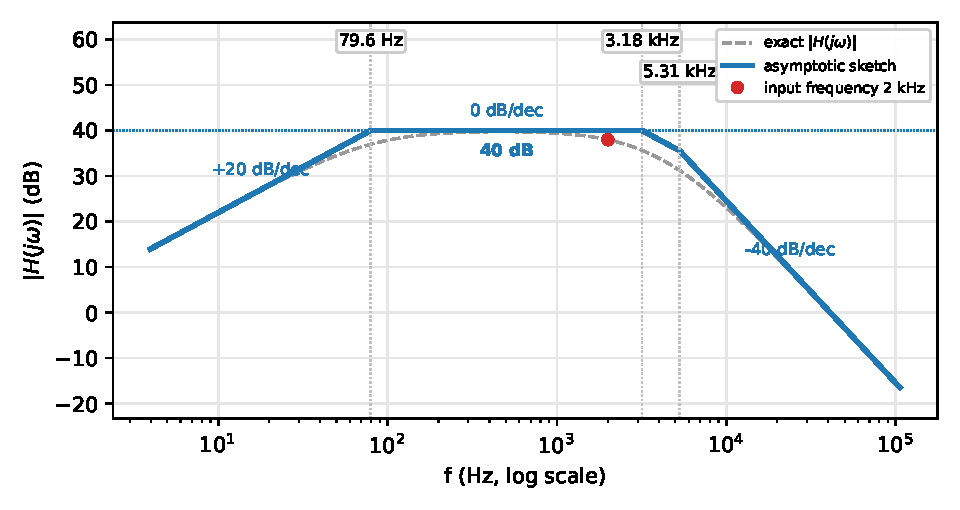
\includegraphics[width=0.78\linewidth,height=6.5cm,keepaspectratio]{p15_bode}\end{center}

{\small Blue: the straight-line sketch you are expected to draw. Dashed grey: the exact curve (about 3\,dB below the corner of an isolated pole). Red dot: the input frequency of Step 7.}
\solstep{7}{Steady-state output}The input is $V_i(t) = 0.1\sin\left(2\pi\cdot 2000\,t+\frac{\pi}{4}\right)$, so $\omega_{in} = 2\pi\cdot 2000 = 12600$\,rad/s. Put $s=j\omega_{in}$ in each factor (tool T5): magnitudes multiply, angles add.
{\small Rules: $\left|\frac{s}{s+p}\right| = \frac{\omega}{\sqrt{\omega^2+p^2}}$, $\angle = \frac{\pi}{2}-\tan^{-1}\frac{\omega}{p}$;\quad $\left|\frac{1}{1+s/p}\right| = \frac{1}{\sqrt{1+(\omega/p)^2}}$, $\angle = -\tan^{-1}\frac{\omega}{p}$;\quad $\left|1+\frac{s}{z}\right| = \sqrt{1+(\omega/z)^2}$, $\angle = \tan^{-1}\frac{\omega}{z}$;\quad a negative $K$ adds $-\pi$.}
\begin{center}\renewcommand{\arraystretch}{1.35}
\begin{tabular}{ccc}
\toprule
factor & magnitude & angle (rad) \\
\midrule
$-100$ & $100$ & $-3.14$ \\
$\rule[-1.1em]{0pt}{2.8em}\dfrac{s}{s+2\pi\cdot 79.6}$ & $0.9992$ & $0.0398$ \\
$\rule[-1.7em]{0pt}{4em}\dfrac{1}{1+\dfrac{s}{2\pi\cdot 3.18\mathrm{k}}}$ & $0.8467$ & $-0.561$ \\
$\rule[-1.7em]{0pt}{4em}\dfrac{1}{1+\dfrac{s}{2\pi\cdot 5.31\mathrm{k}}}$ & $0.9357$ & $-0.361$ \\
\textbf{total} & $\mathbf{79.17}$ (product) & $\mathbf{-4.02}$ (sum) \\
\bottomrule
\end{tabular}\end{center}

\begin{align*}
|H(j\omega_{in})| &= 79.2, \qquad \angle H(j\omega_{in}) = -4.02\ \mathrm{rad} \\
v_{o,ac}(t) &= 79.2\times 0.1\,\sin\left(2\pi\cdot 2000\,t - 3.24\right) = 7.92\,\sin\left(2\pi\cdot 2000\,t - 3.24\right)
\end{align*}

(phase: $\theta + \angle H = \frac{\pi}{4} + (-4.02) = -3.24$\,rad.)
\[
\boxed{V_o(t) = 7.92\,\sin\left(2\pi\cdot 2000\,t - 3.24\right)\ \mathrm{V}}
\]

\begin{ansbox}
$H(s) = -100\,\dfrac{s}{s+2\pi\cdot 79.6}\,\dfrac{1}{1+\dfrac{s}{2\pi\cdot 3.18\mathrm{k}}}\,\dfrac{1}{1+\dfrac{s}{2\pi\cdot 5.31\mathrm{k}}}$\quad (corners: 79.6 Hz, 3.18 kHz, 5.31 kHz)\\[4pt]
$V_o(t) = 7.92\,\sin\left(2\pi\cdot 2000\,t - 3.24\right)\ \mathrm{V}$
\end{ansbox}

\newpage
\subsection*{Solution 1C.16 \hfill Hard}
\begin{center}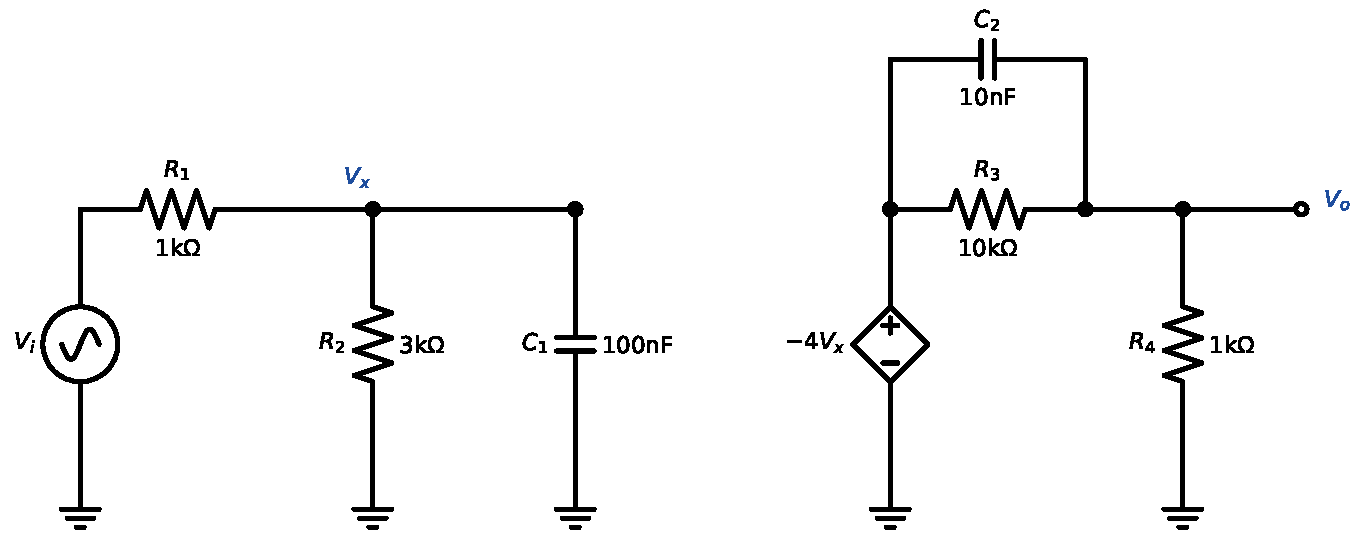
\includegraphics[width=0.8\linewidth,height=4.5cm,keepaspectratio]{p16_circuit}\end{center}
\solstep{1}{Identify the sources}Independent sources: the AC input $V_i(t)$. The diamond-shaped sources are \emph{dependent} sources: they are not inputs, they only copy/scale a voltage that already exists in the circuit, so they stay in the circuit in every step. There is no DC source, so $V_{o,dc}=0$ and $V_o(t)=v_{o,ac}(t)$: Step 2 is skipped.
\solstep{2}{DC circuit}No DC sources: $V_{o,dc}=0$.
\solstep{3}{AC circuit}Replace every capacitor by $\frac{1}{sC}$ and every inductor by $sL$.
AC equivalent circuit (nodes named for the next step):
\begin{center}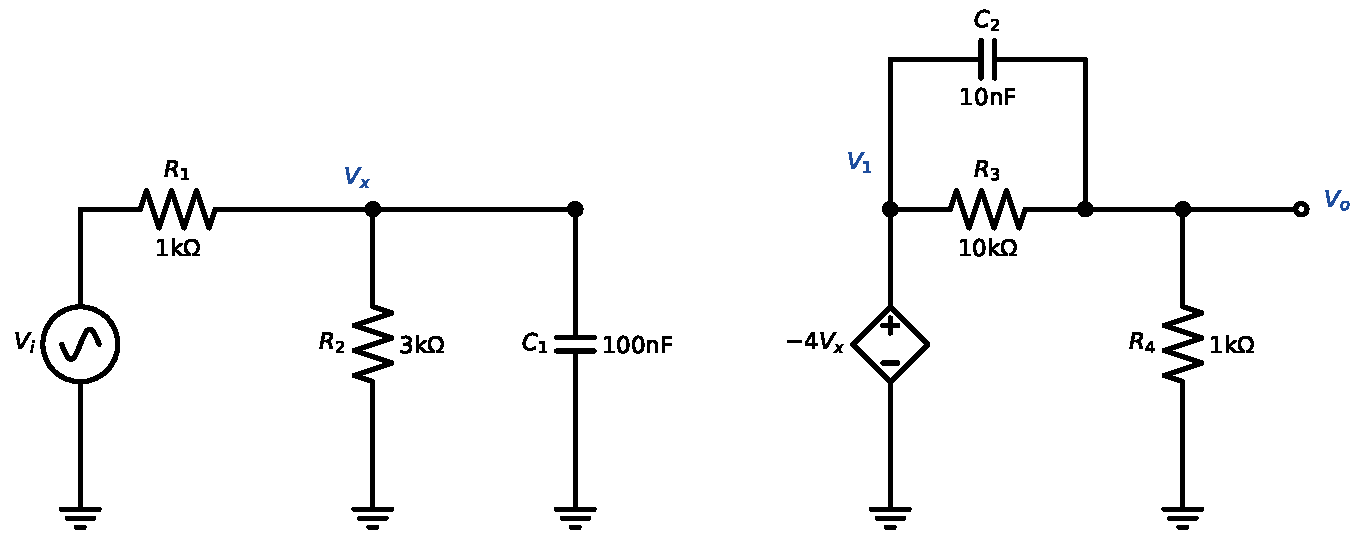
\includegraphics[width=0.95\linewidth,height=5.2cm,keepaspectratio]{p16_ac}\end{center}

\solstep{4}{Transfer function by a chain of dividers}Walk from the input to the output through the named nodes: $V_{i} \to V_{x} \to V_{1} \to V_{o}$. The transfer function is the product of the node-to-node ratios (each one is a simple divider, tool T2, or a dependent source, tool T4):
\[
H(s) = \frac{V_o}{V_i} = \frac{V_{x}}{V_{i}}\cdot\frac{V_{1}}{V_{x}}\cdot\frac{V_{o}}{V_{1}}
\]

Impedances seen \emph{looking right} from a node (everything from that node to ground, excluding what is on its left). Compute them from the far right toward the input:
\begin{align*}
Z_{x} &= R_{2} \parallel \frac{1}{sC_{1}} = \dfrac{10^{7}}{s + 3330}
\end{align*}

Now each link. {\small (Algebra tip: to simplify a fraction that contains fractions, multiply its top and bottom by every inner denominator; then divide top and bottom by the leading coefficient of the denominator so that it starts with a plain $s^n$.)}
\begin{align*}
\frac{V_{x}}{V_{i}} &= \frac{Z_{x}}{R_{1} + Z_{x}} = \dfrac{10000}{s + 13300} \\
\frac{V_{1}}{V_{x}} &= -4 &&\text{(ideal VCVS: $V_{1} = -4V_{x}$)} \\
\frac{V_{o}}{V_{1}} &= \frac{R_{4}}{R_{3} \parallel \frac{1}{sC_{2}} + R_{4}} = \dfrac{s + 10000}{s + 1.1\times 10^{5}}
\end{align*}

Multiply the links and simplify (common factors cancel):\[
H(s) = \dfrac{-40000\,s - 4\times 10^{8}}{s^{2} + 1.23\times 10^{5}\,s + 1.47\times 10^{9}}
\]

\solstep{5}{Standard (Bode-ready) form}Find the roots. Every root $s=-p$ of the denominator is a \emph{pole}, every root $s=-z$ of the numerator is a \emph{zero}; $|p|$ and $|z|$ are the corner frequencies (rad/s).
\begin{itemize}[leftmargin=*,itemsep=2pt]
\item Numerator: $-40000\,s - 4\times 10^{8}$; divide by the leading coefficient $-40000$ (this does not move the roots): $s + 10000$; $s + 10000 = 0 \Rightarrow s = -10000$.
\item Denominator: $s^{2} + 1.23\times 10^{5}\,s + 1.47\times 10^{9}$; quadratic formula:\[
s = \frac{-1.23\times 10^{5} \pm \sqrt{(1.23\times 10^{5})^2 - 4(1.47\times 10^{9})}}{2} = \frac{-1.23\times 10^{5} \pm 96700}{2} \Rightarrow s = -13300,\ -1.1\times 10^{5}
\]

\end{itemize}

Factored form (leading coefficient in front):
\[
H(s) = -40000\,\dfrac{(s+10000)}{(s+13300)(s+1.1\times 10^{5})}
\]

Bode-ready form: rewrite every $(s+p) = p\left(1+\frac{s}{p}\right)$ and $(s+z) = z\left(1+\frac{s}{z}\right)$, and collect all constants into $K$. Then every factor except $K$ is $\approx 1$ inside the pass-band:
\[
H(s) = -0.273\,\left(1+\dfrac{s}{2\pi\cdot 1.59\mathrm{k}}\right)\,\dfrac{1}{1+\dfrac{s}{2\pi\cdot 2.12\mathrm{k}}}\,\dfrac{1}{1+\dfrac{s}{2\pi\cdot 17.5\mathrm{k}}},\qquad K = -0.273
\]

\begin{center}\renewcommand{\arraystretch}{1.35}
\begin{tabular}{cccc}
\toprule
type & $\omega_c$ (rad/s) & $f_c=\omega_c/2\pi$ & slope change \\
\midrule
zero & $10000$ & 1.59 kHz & $+20$ dB/dec \\
pole & $13300$ & 2.12 kHz & $-20$ dB/dec \\
pole & $1.1\times 10^{5}$ & 17.5 kHz & $-20$ dB/dec \\
\bottomrule
\end{tabular}\end{center}

\solstep{6}{Magnitude Bode plot}Below every corner, all factors are $\approx$ constant: $|H| \approx 0.273$ $= -11.3$\,dB (flat, 0 dB/dec). Then, moving right, each pole bends the line down by 20\,dB/dec and each zero bends it up by 20\,dB/dec (tool T6):
\begin{center}\renewcommand{\arraystretch}{1.35}
\begin{tabular}{lcl}
\toprule
frequency range & slope & asymptote level \\
\midrule
$f<$ 1.59 kHz & $0$ dB/dec (flat) & -11.3 dB at end \\
1.59 kHz -- 2.12 kHz & $+20$ dB/dec & -11.3 dB at start, -8.79 dB at end \\
2.12 kHz -- 17.5 kHz & $0$ dB/dec (flat) & -8.79 dB at start, -8.79 dB at end \\
$f>$ 17.5 kHz & $-20$ dB/dec & -8.79 dB at start \\
\bottomrule
\end{tabular}\end{center}

\begin{center}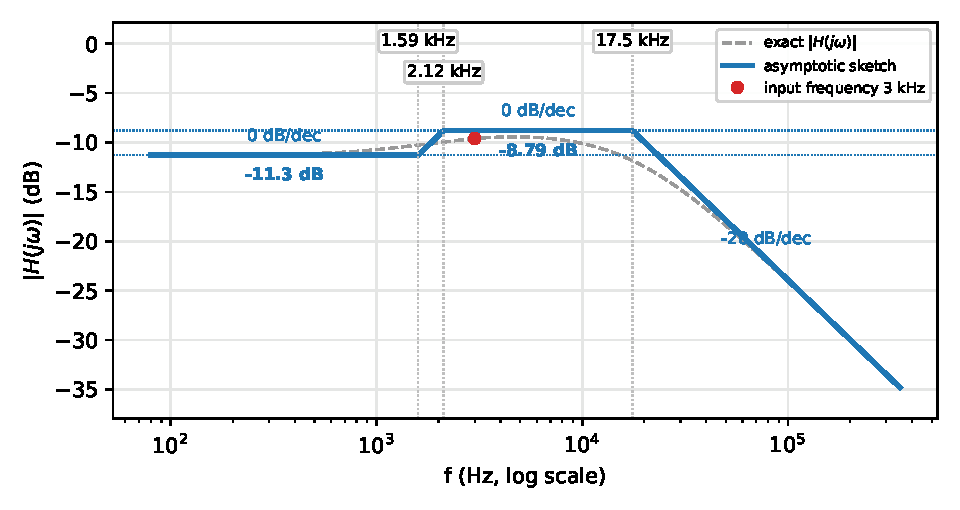
\includegraphics[width=0.78\linewidth,height=6.5cm,keepaspectratio]{p16_bode}\end{center}

{\small Blue: the straight-line sketch you are expected to draw. Dashed grey: the exact curve (about 3\,dB below the corner of an isolated pole). Red dot: the input frequency of Step 7.}
\solstep{7}{Steady-state output}The input is $V_i(t) = 0.1\cos\left(2\pi\cdot 3000\,t\right)$, so $\omega_{in} = 2\pi\cdot 3000 = 18800$\,rad/s. Put $s=j\omega_{in}$ in each factor (tool T5): magnitudes multiply, angles add.
{\small Rules: $\left|\frac{s}{s+p}\right| = \frac{\omega}{\sqrt{\omega^2+p^2}}$, $\angle = \frac{\pi}{2}-\tan^{-1}\frac{\omega}{p}$;\quad $\left|\frac{1}{1+s/p}\right| = \frac{1}{\sqrt{1+(\omega/p)^2}}$, $\angle = -\tan^{-1}\frac{\omega}{p}$;\quad $\left|1+\frac{s}{z}\right| = \sqrt{1+(\omega/z)^2}$, $\angle = \tan^{-1}\frac{\omega}{z}$;\quad a negative $K$ adds $-\pi$.}
\begin{center}\renewcommand{\arraystretch}{1.35}
\begin{tabular}{ccc}
\toprule
factor & magnitude & angle (rad) \\
\midrule
$-0.273$ & $0.2727$ & $-3.14$ \\
$\rule[-1.1em]{0pt}{2.8em}\left(1+\dfrac{s}{2\pi\cdot 1.59\mathrm{k}}\right)$ & $2.134$ & $1.08$ \\
$\rule[-1.7em]{0pt}{4em}\dfrac{1}{1+\dfrac{s}{2\pi\cdot 2.12\mathrm{k}}}$ & $0.5775$ & $-0.955$ \\
$\rule[-1.7em]{0pt}{4em}\dfrac{1}{1+\dfrac{s}{2\pi\cdot 17.5\mathrm{k}}}$ & $0.9856$ & $-0.17$ \\
\textbf{total} & $\mathbf{0.3312}$ (product) & $\mathbf{-3.18}$ (sum) \\
\bottomrule
\end{tabular}\end{center}

\begin{align*}
|H(j\omega_{in})| &= 0.331, \qquad \angle H(j\omega_{in}) = -3.18\ \mathrm{rad} \\
v_{o,ac}(t) &= 0.331\times 0.1\,\cos\left(2\pi\cdot 3000\,t - 3.18\right) = 0.0331\,\cos\left(2\pi\cdot 3000\,t - 3.18\right)
\end{align*}

\[
\boxed{V_o(t) = 0.0331\,\cos\left(2\pi\cdot 3000\,t - 3.18\right)\ \mathrm{V}}
\]

\begin{ansbox}
$H(s) = -0.273\,\left(1+\dfrac{s}{2\pi\cdot 1.59\mathrm{k}}\right)\,\dfrac{1}{1+\dfrac{s}{2\pi\cdot 2.12\mathrm{k}}}\,\dfrac{1}{1+\dfrac{s}{2\pi\cdot 17.5\mathrm{k}}}$\quad (corners: 1.59 kHz, 2.12 kHz, 17.5 kHz)\\[4pt]
$V_o(t) = 0.0331\,\cos\left(2\pi\cdot 3000\,t - 3.18\right)\ \mathrm{V}$
\end{ansbox}

\newpage
\subsection*{Solution 1C.17 \hfill Hard}
\begin{center}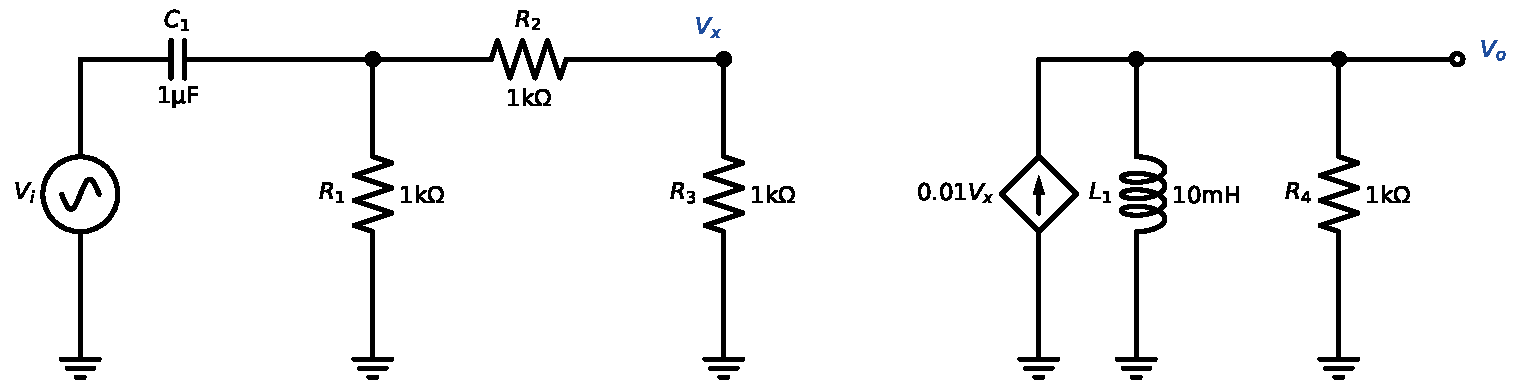
\includegraphics[width=0.8\linewidth,height=4.5cm,keepaspectratio]{p17_circuit}\end{center}
\solstep{1}{Identify the sources}Independent sources: the AC input $V_i(t)$. The diamond-shaped sources are \emph{dependent} sources: they are not inputs, they only copy/scale a voltage that already exists in the circuit, so they stay in the circuit in every step. There is no DC source, so $V_{o,dc}=0$ and $V_o(t)=v_{o,ac}(t)$: Step 2 is skipped.
\solstep{2}{DC circuit}No DC sources: $V_{o,dc}=0$.
\solstep{3}{AC circuit}Replace every capacitor by $\frac{1}{sC}$ and every inductor by $sL$.
AC equivalent circuit (nodes named for the next step):
\begin{center}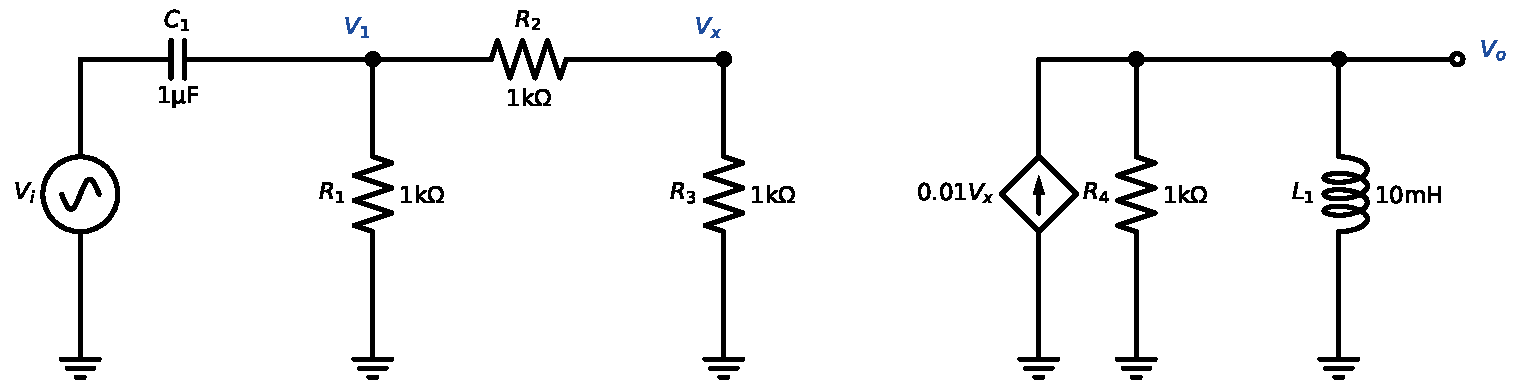
\includegraphics[width=0.95\linewidth,height=5.2cm,keepaspectratio]{p17_ac}\end{center}

\solstep{4}{Transfer function by a chain of dividers}Walk from the input to the output through the named nodes: $V_{i} \to V_{1} \to V_{x} \to V_{o}$. The transfer function is the product of the node-to-node ratios (each one is a simple divider, tool T2, or a dependent source, tool T4):
\[
H(s) = \frac{V_o}{V_i} = \frac{V_{1}}{V_{i}}\cdot\frac{V_{x}}{V_{1}}\cdot\frac{V_{o}}{V_{x}}
\]

Impedances seen \emph{looking right} from a node (everything from that node to ground, excluding what is on its left). Compute them from the far right toward the input:
\begin{align*}
Z_{1} &= R_{1} \parallel \left(R_{2} + R_{3}\right) = 667 \\
Z_{o} &= R_{4} \parallel sL_{1} = \dfrac{1000\,s}{s + 10^{5}}
\end{align*}

Now each link. {\small (Algebra tip: to simplify a fraction that contains fractions, multiply its top and bottom by every inner denominator; then divide top and bottom by the leading coefficient of the denominator so that it starts with a plain $s^n$.)}
\begin{align*}
\frac{V_{1}}{V_{i}} &= \frac{Z_{1}}{\frac{1}{sC_{1}} + Z_{1}} = \dfrac{s}{s + 1500} \\
\frac{V_{x}}{V_{1}} &= \frac{R_{3}}{R_{2} + R_{3}} = 0.5 \\
\frac{V_{o}}{V_{x}} &= 0.01\,Z_{o} = \dfrac{10\,s}{s + 10^{5}}
\end{align*}

(VCCS: the current $0.01V_{x}$ flows into node $V_{o}$ and through $Z_{o}$ to ground, so $V_{o} = 0.01V_{x}\,Z_{o}$ by Ohm's law.)
Multiply the links and simplify (common factors cancel):\[
H(s) = \dfrac{5\,s^{2}}{s^{2} + 1.01\times 10^{5}\,s + 1.5\times 10^{8}}
\]

\solstep{5}{Standard (Bode-ready) form}Find the roots. Every root $s=-p$ of the denominator is a \emph{pole}, every root $s=-z$ of the numerator is a \emph{zero}; $|p|$ and $|z|$ are the corner frequencies (rad/s).
\begin{itemize}[leftmargin=*,itemsep=2pt]
\item Numerator: it has the factor $s^2$ $\Rightarrow$ 2 zeros at $s=0$.
\item Denominator: $s^{2} + 1.01\times 10^{5}\,s + 1.5\times 10^{8}$; quadratic formula:\[
s = \frac{-1.01\times 10^{5} \pm \sqrt{(1.01\times 10^{5})^2 - 4(1.5\times 10^{8})}}{2} = \frac{-1.01\times 10^{5} \pm 98500}{2} \Rightarrow s = -1500,\ -10^{5}
\]

\end{itemize}

Factored form (leading coefficient in front):
\[
H(s) = 5\,\dfrac{s^{2}}{(s+1500)(s+10^{5})}
\]

Bode-ready form: rewrite every $(s+p) = p\left(1+\frac{s}{p}\right)$ and $(s+z) = z\left(1+\frac{s}{z}\right)$, and collect all constants into $K$. Each $s$ in the numerator is paired with one of the \emph{lowest} poles as $\frac{s}{s+p}$ (that factor is $\approx 1$ above $p$). Then every factor except $K$ is $\approx 1$ inside the pass-band:
\[
H(s) = 5\,\dfrac{s}{s+2\pi\cdot 239}\,\dfrac{s}{s+2\pi\cdot 15.9\mathrm{k}},\qquad K = 5
\]

\begin{center}\renewcommand{\arraystretch}{1.35}
\begin{tabular}{cccc}
\toprule
type & $\omega_c$ (rad/s) & $f_c=\omega_c/2\pi$ & slope change \\
\midrule
pole & $1500$ & 239 Hz & $-20$ dB/dec \\
pole & $10^{5}$ & 15.9 kHz & $-20$ dB/dec \\
\bottomrule
\end{tabular}\end{center}

\solstep{6}{Magnitude Bode plot}Below every corner $|H(s)|\approx 3.33\times 10^{-8}\,s^2$, so the plot starts with a slope of $+40$\,dB/dec. Then, moving right, each pole bends the line down by 20\,dB/dec and each zero bends it up by 20\,dB/dec (tool T6):
\begin{center}\renewcommand{\arraystretch}{1.35}
\begin{tabular}{lcl}
\toprule
frequency range & slope & asymptote level \\
\midrule
$f<$ 239 Hz & $+40$ dB/dec & -22.5 dB at end \\
239 Hz -- 15.9 kHz & $+20$ dB/dec & -22.5 dB at start, 14 dB at end \\
$f>$ 15.9 kHz & $0$ dB/dec (flat) & 14 dB at start \\
\bottomrule
\end{tabular}\end{center}

The flat (pass-band) level is $20\log_{10}|K| = 20\log_{10}5 = 14$\,dB.
\begin{center}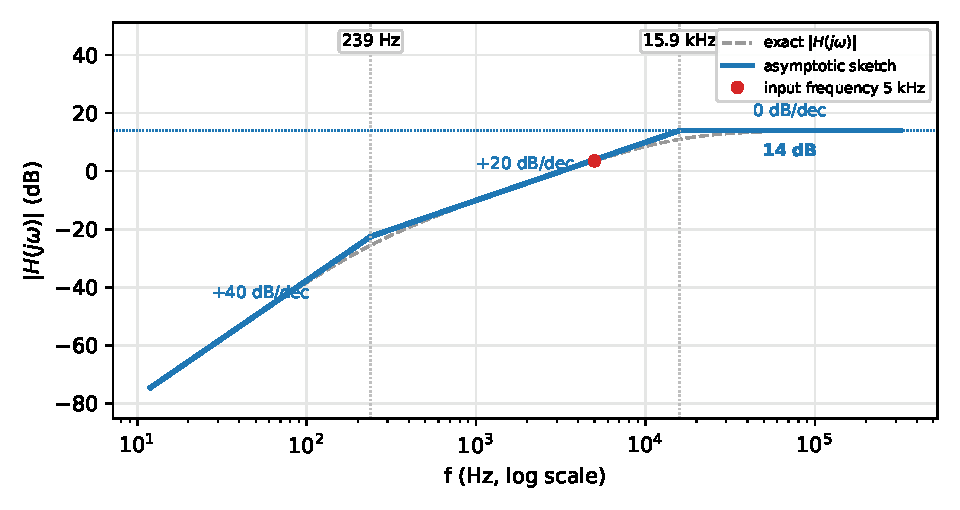
\includegraphics[width=0.78\linewidth,height=6.5cm,keepaspectratio]{p17_bode}\end{center}

{\small Blue: the straight-line sketch you are expected to draw. Dashed grey: the exact curve (about 3\,dB below the corner of an isolated pole). Red dot: the input frequency of Step 7.}
\solstep{7}{Steady-state output}The input is $V_i(t) = 0.2\sin\left(2\pi\cdot 5000\,t-\frac{\pi}{6}\right)$, so $\omega_{in} = 2\pi\cdot 5000 = 31400$\,rad/s. Put $s=j\omega_{in}$ in each factor (tool T5): magnitudes multiply, angles add.
{\small Rules: $\left|\frac{s}{s+p}\right| = \frac{\omega}{\sqrt{\omega^2+p^2}}$, $\angle = \frac{\pi}{2}-\tan^{-1}\frac{\omega}{p}$;\quad $\left|\frac{1}{1+s/p}\right| = \frac{1}{\sqrt{1+(\omega/p)^2}}$, $\angle = -\tan^{-1}\frac{\omega}{p}$;\quad $\left|1+\frac{s}{z}\right| = \sqrt{1+(\omega/z)^2}$, $\angle = \tan^{-1}\frac{\omega}{z}$;\quad a negative $K$ adds $-\pi$.}
\begin{center}\renewcommand{\arraystretch}{1.35}
\begin{tabular}{ccc}
\toprule
factor & magnitude & angle (rad) \\
\midrule
$5$ & $5$ & $0$ \\
$\rule[-1.1em]{0pt}{2.8em}\dfrac{s}{s+2\pi\cdot 239}$ & $0.9989$ & $0.0477$ \\
$\rule[-1.1em]{0pt}{2.8em}\dfrac{s}{s+2\pi\cdot 15.9\mathrm{k}}$ & $0.2997$ & $1.27$ \\
\textbf{total} & $\mathbf{1.497}$ (product) & $\mathbf{1.31}$ (sum) \\
\bottomrule
\end{tabular}\end{center}

\begin{align*}
|H(j\omega_{in})| &= 1.5, \qquad \angle H(j\omega_{in}) = 1.31\ \mathrm{rad} \\
v_{o,ac}(t) &= 1.5\times 0.2\,\sin\left(2\pi\cdot 5000\,t + 0.791\right) = 0.299\,\sin\left(2\pi\cdot 5000\,t + 0.791\right)
\end{align*}

(phase: $\theta + \angle H = -\frac{\pi}{6} + (1.31) = 0.791$\,rad.)
\[
\boxed{V_o(t) = 0.299\,\sin\left(2\pi\cdot 5000\,t + 0.791\right)\ \mathrm{V}}
\]

\begin{ansbox}
$H(s) = 5\,\dfrac{s}{s+2\pi\cdot 239}\,\dfrac{s}{s+2\pi\cdot 15.9\mathrm{k}}$\quad (corners: 239 Hz, 15.9 kHz)\\[4pt]
$V_o(t) = 0.299\,\sin\left(2\pi\cdot 5000\,t + 0.791\right)\ \mathrm{V}$
\end{ansbox}

\newpage
\subsection*{Solution 1C.18 \hfill Hard}
\begin{center}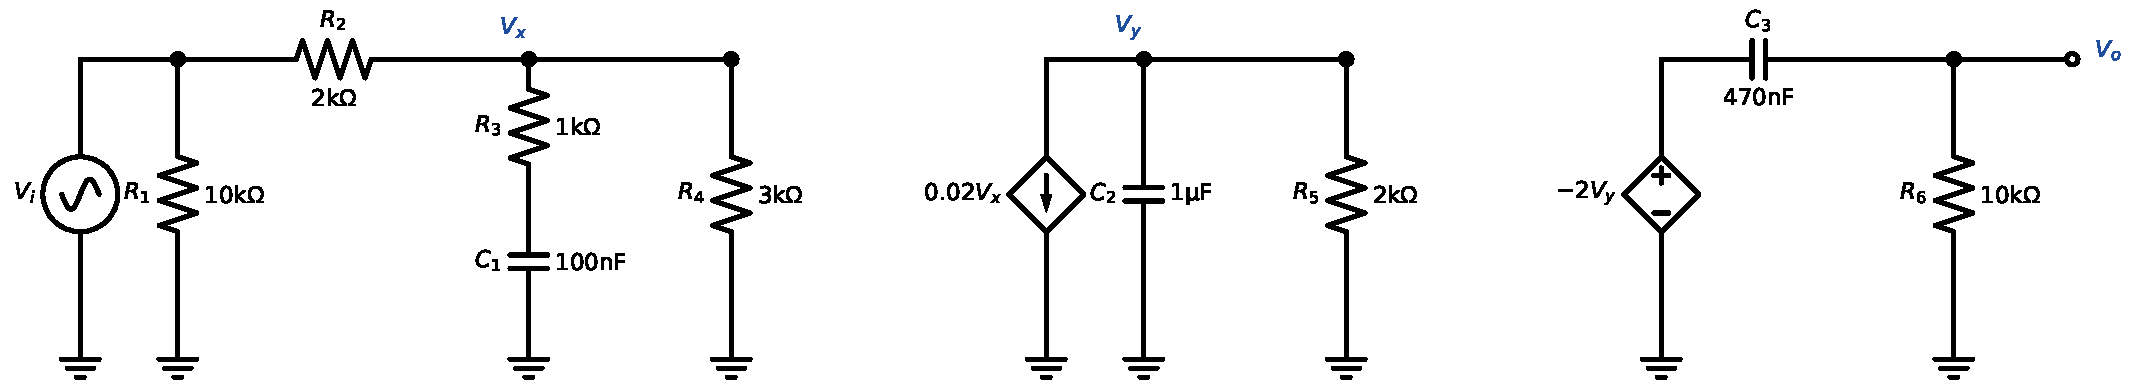
\includegraphics[width=0.8\linewidth,height=4.5cm,keepaspectratio]{p18_circuit}\end{center}
\solstep{1}{Identify the sources}Independent sources: the AC input $V_i(t)$. The diamond-shaped sources are \emph{dependent} sources: they are not inputs, they only copy/scale a voltage that already exists in the circuit, so they stay in the circuit in every step. There is no DC source, so $V_{o,dc}=0$ and $V_o(t)=v_{o,ac}(t)$: Step 2 is skipped.
\solstep{2}{DC circuit}No DC sources: $V_{o,dc}=0$.
\solstep{3}{AC circuit}Replace every capacitor by $\frac{1}{sC}$ and every inductor by $sL$.
\begin{itemize}[leftmargin=*,itemsep=2pt]
\item $R_{1}$ sits directly across the ideal input source $V_i$. An ideal voltage source keeps its voltage whatever you connect to it, so $R_{1}$ cannot change any node voltage: it drops out of $H(s)$.
\end{itemize}

AC equivalent circuit (nodes named for the next step):
\begin{center}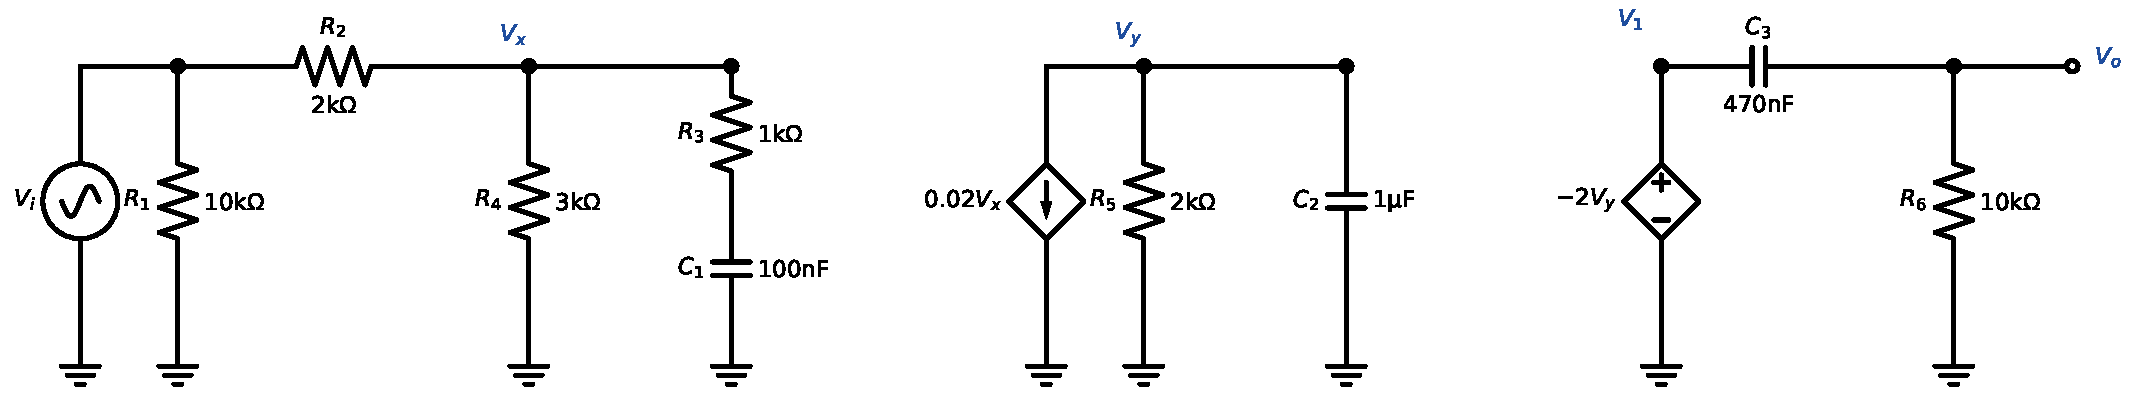
\includegraphics[width=0.95\linewidth,height=5.2cm,keepaspectratio]{p18_ac}\end{center}

\solstep{4}{Transfer function by a chain of dividers}Walk from the input to the output through the named nodes: $V_{i} \to V_{x} \to V_{y} \to V_{1} \to V_{o}$. The transfer function is the product of the node-to-node ratios (each one is a simple divider, tool T2, or a dependent source, tool T4):
\[
H(s) = \frac{V_o}{V_i} = \frac{V_{x}}{V_{i}}\cdot\frac{V_{y}}{V_{x}}\cdot\frac{V_{1}}{V_{y}}\cdot\frac{V_{o}}{V_{1}}
\]

Impedances seen \emph{looking right} from a node (everything from that node to ground, excluding what is on its left). Compute them from the far right toward the input:
\begin{align*}
Z_{x} &= R_{4} \parallel \left(R_{3} + \frac{1}{sC_{1}}\right) = \dfrac{750\,s + 7.5\times 10^{6}}{s + 2500} \\
Z_{y} &= R_{5} \parallel \frac{1}{sC_{2}} = \dfrac{10^{6}}{s + 500}
\end{align*}

Now each link. {\small (Algebra tip: to simplify a fraction that contains fractions, multiply its top and bottom by every inner denominator; then divide top and bottom by the leading coefficient of the denominator so that it starts with a plain $s^n$.)}
\begin{align*}
\frac{V_{x}}{V_{i}} &= \frac{Z_{x}}{R_{2} + Z_{x}} = \dfrac{0.273\,s + 2730}{s + 4550} \\
\frac{V_{y}}{V_{x}} &= -0.02\,Z_{y} = \dfrac{-20000}{s + 500} \\
\frac{V_{1}}{V_{y}} &= -2 &&\text{(ideal VCVS: $V_{1} = -2V_{y}$)} \\
\frac{V_{o}}{V_{1}} &= \frac{R_{6}}{\frac{1}{sC_{3}} + R_{6}} = \dfrac{s}{s + 213}
\end{align*}

(VCCS: the current $0.02V_{x}$ flows out of node $V_{y}$ and through $Z_{y}$ to ground, so $V_{y} = -0.02V_{x}\,Z_{y}$ by Ohm's law.)
Multiply the links and simplify (common factors cancel):\[
H(s) = \dfrac{10900\,s^{2} + 1.09\times 10^{8}\,s}{s^{3} + 5260\,s^{2} + 3.35\times 10^{6}\,s + 4.84\times 10^{8}}
\]

\solstep{5}{Standard (Bode-ready) form}Find the roots. Every root $s=-p$ of the denominator is a \emph{pole}, every root $s=-z$ of the numerator is a \emph{zero}; $|p|$ and $|z|$ are the corner frequencies (rad/s).
\begin{itemize}[leftmargin=*,itemsep=2pt]
\item Numerator: it has the factor $s$ $\Rightarrow$ 1 zero at $s=0$.
\item Numerator (after taking out the $s$ factor): $10900\,s + 1.09\times 10^{8}$; divide by the leading coefficient $10900$ (this does not move the roots): $s + 10000$; $s + 10000 = 0 \Rightarrow s = -10000$.
\item Denominator: $s^{3} + 5260\,s^{2} + 3.35\times 10^{6}\,s + 4.84\times 10^{8}$; this is degree 3: use a calculator's polynomial solver (or \texttt{numpy.roots}) $\Rightarrow s = -213,\ -500,\ -4550$.
\end{itemize}

Factored form (leading coefficient in front):
\[
H(s) = 10900\,\dfrac{s(s+10000)}{(s+213)(s+500)(s+4550)}
\]

Bode-ready form: rewrite every $(s+p) = p\left(1+\frac{s}{p}\right)$ and $(s+z) = z\left(1+\frac{s}{z}\right)$, and collect all constants into $K$. Each $s$ in the numerator is paired with one of the \emph{lowest} poles as $\frac{s}{s+p}$ (that factor is $\approx 1$ above $p$). Then every factor except $K$ is $\approx 1$ inside the pass-band:
\[
H(s) = 48\,\dfrac{s}{s+2\pi\cdot 33.9}\,\dfrac{1}{1+\dfrac{s}{2\pi\cdot 79.6}}\,\dfrac{1}{1+\dfrac{s}{2\pi\cdot 723}}\,\left(1+\dfrac{s}{2\pi\cdot 1.59\mathrm{k}}\right),\qquad K = 48
\]

\begin{center}\renewcommand{\arraystretch}{1.35}
\begin{tabular}{cccc}
\toprule
type & $\omega_c$ (rad/s) & $f_c=\omega_c/2\pi$ & slope change \\
\midrule
pole & $213$ & 33.9 Hz & $-20$ dB/dec \\
pole & $500$ & 79.6 Hz & $-20$ dB/dec \\
pole & $4550$ & 723 Hz & $-20$ dB/dec \\
zero & $10000$ & 1.59 kHz & $+20$ dB/dec \\
\bottomrule
\end{tabular}\end{center}

\solstep{6}{Magnitude Bode plot}Below every corner $|H(s)|\approx 0.226\,s$, so the plot starts with a slope of $+20$\,dB/dec. Then, moving right, each pole bends the line down by 20\,dB/dec and each zero bends it up by 20\,dB/dec (tool T6):
\begin{center}\renewcommand{\arraystretch}{1.35}
\begin{tabular}{lcl}
\toprule
frequency range & slope & asymptote level \\
\midrule
$f<$ 33.9 Hz & $+20$ dB/dec & 33.6 dB at end \\
33.9 Hz -- 79.6 Hz & $0$ dB/dec (flat) & 33.6 dB at start, 33.6 dB at end \\
79.6 Hz -- 723 Hz & $-20$ dB/dec & 33.6 dB at start, 14.5 dB at end \\
723 Hz -- 1.59 kHz & $-40$ dB/dec & 14.5 dB at start, 0.756 dB at end \\
$f>$ 1.59 kHz & $-20$ dB/dec & 0.756 dB at start \\
\bottomrule
\end{tabular}\end{center}

\begin{center}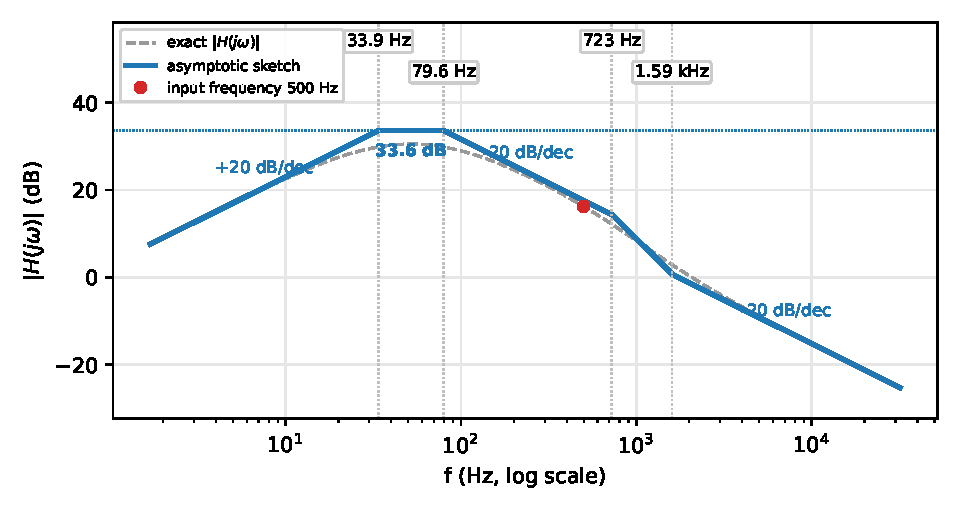
\includegraphics[width=0.78\linewidth,height=6.5cm,keepaspectratio]{p18_bode}\end{center}

{\small Blue: the straight-line sketch you are expected to draw. Dashed grey: the exact curve (about 3\,dB below the corner of an isolated pole). Red dot: the input frequency of Step 7.}
\solstep{7}{Steady-state output}The input is $V_i(t) = 0.01\cos\left(2\pi\cdot 500\,t+\frac{\pi}{3}\right)$, so $\omega_{in} = 2\pi\cdot 500 = 3140$\,rad/s. Put $s=j\omega_{in}$ in each factor (tool T5): magnitudes multiply, angles add.
{\small Rules: $\left|\frac{s}{s+p}\right| = \frac{\omega}{\sqrt{\omega^2+p^2}}$, $\angle = \frac{\pi}{2}-\tan^{-1}\frac{\omega}{p}$;\quad $\left|\frac{1}{1+s/p}\right| = \frac{1}{\sqrt{1+(\omega/p)^2}}$, $\angle = -\tan^{-1}\frac{\omega}{p}$;\quad $\left|1+\frac{s}{z}\right| = \sqrt{1+(\omega/z)^2}$, $\angle = \tan^{-1}\frac{\omega}{z}$;\quad a negative $K$ adds $-\pi$.}
\begin{center}\renewcommand{\arraystretch}{1.35}
\begin{tabular}{ccc}
\toprule
factor & magnitude & angle (rad) \\
\midrule
$48$ & $48$ & $0$ \\
$\rule[-1.1em]{0pt}{2.8em}\dfrac{s}{s+2\pi\cdot 33.9}$ & $0.9977$ & $0.0676$ \\
$\rule[-1.7em]{0pt}{4em}\dfrac{1}{1+\dfrac{s}{2\pi\cdot 79.6}}$ & $0.1572$ & $-1.41$ \\
$\rule[-1.7em]{0pt}{4em}\dfrac{1}{1+\dfrac{s}{2\pi\cdot 723}}$ & $0.8226$ & $-0.605$ \\
$\rule[-1.1em]{0pt}{2.8em}\left(1+\dfrac{s}{2\pi\cdot 1.59\mathrm{k}}\right)$ & $1.048$ & $0.304$ \\
\textbf{total} & $\mathbf{6.491}$ (product) & $\mathbf{-1.65}$ (sum) \\
\bottomrule
\end{tabular}\end{center}

\begin{align*}
|H(j\omega_{in})| &= 6.49, \qquad \angle H(j\omega_{in}) = -1.65\ \mathrm{rad} \\
v_{o,ac}(t) &= 6.49\times 0.01\,\cos\left(2\pi\cdot 500\,t - 0.599\right) = 0.0649\,\cos\left(2\pi\cdot 500\,t - 0.599\right)
\end{align*}

(phase: $\theta + \angle H = \frac{\pi}{3} + (-1.65) = -0.599$\,rad.)
\[
\boxed{V_o(t) = 0.0649\,\cos\left(2\pi\cdot 500\,t - 0.599\right)\ \mathrm{V}}
\]

\begin{ansbox}
$H(s) = 48\,\dfrac{s}{s+2\pi\cdot 33.9}\,\dfrac{1}{1+\dfrac{s}{2\pi\cdot 79.6}}\,\dfrac{1}{1+\dfrac{s}{2\pi\cdot 723}}\,\left(1+\dfrac{s}{2\pi\cdot 1.59\mathrm{k}}\right)$\quad (corners: 33.9 Hz, 79.6 Hz, 723 Hz, 1.59 kHz)\\[4pt]
$V_o(t) = 0.0649\,\cos\left(2\pi\cdot 500\,t - 0.599\right)\ \mathrm{V}$
\end{ansbox}

\end{document}
